\documentclass{mythesis}
\usepackage{mythesis}

% my packages
\usepackage{color}
\usepackage[printonlyused]{acronym}
\usepackage{hyperref}
\usepackage{slashed}
\usepackage{draftwatermark}
\SetWatermarkScale{8.}
\SetWatermarkLightness{0.9}
\SetWatermarkFontSize{60cm}

% my commands
\newcommand{\rnine}{\ensuremath{R_{9}}\xspace}
\newcommand{\comm}[1]{\textcolor{red}{#1}\xspace}
\newcommand{\Hgg}{\ensuremath{H\rightarrow\gamma\gamma}\xspace}
\newcommand{\mH}{\ensuremath{m_{H}}\xspace}
\newcommand{\fb}{\ensuremath{fb^{-1}}\xspace}
\newcommand{\mgg}{\ensuremath{m_{\gamma\gamma}}\xspace}
\newcommand{\HZZ}{\ensuremath{H\rightarrow ZZ* \rightarrow l^{+}l^{-}l^{+}l^{-}}\xspace}
\newcommand{\Zee}{\ensuremath{Z\rightarrow e^{+}e^{-}}\xspace}
\newcommand{\Zmumu}{\ensuremath{Z\rightarrow \mu^{+}\mu^{-}}\xspace}
\newcommand{\Zmumugamma}{\ensuremath{Z\rightarrow \mu^{+}\mu^{-}\gamma}\xspace}
\newcommand{\ET}{\ensuremath{E_{T}}\xspace}
%\renewcommand{\pT}{\ensuremath{p_{T}}\xpsace}
\newcommand{\red}[1]{\textcolor{red}{#1}\xspace}
\mathchardef\mhyphen="2D
\newcommand{\pp}{\ensuremath{p \mhyphen p}\xspace}
\newcommand{\pizero}{\ensuremath{\pi^{0}}\xspace}
\newcommand{\MET}{\ensuremath{\slashed{E}_{T}}\xspace}
\newcommand{\graviton}{\ensuremath{2_{m}^{+}}\xspace}
\newcommand{\POWHEG}{\textsc{powheg}\xspace}
\newcommand{\PYTHIA}{\textsc{pythia}\xspace}
\newcommand{\JHU}{\textsc{JHU}\xspace}
\newcommand{\SHERPA}{\textsc{sherpa}\xspace}
\newcommand{\MADGRAPH}{\textsc{MadGraph}\xspace}
\newcommand{\GEANT}{\textsc{Geant4}\xspace}
%\newcommand{\fb}{fb\ensuremath{^{-1}}\xpsace}
\newcommand{\refrqd}{\red{[REF!]}}
% --- acros ---
\renewcommand{\LHC}{\ac{LHC}\xspace}
\renewcommand{\CMS}{\ac{CMS}\xspace}
\newcommand{\ECAL}{\ac{ECAL}\xspace}
\newcommand{\HCAL}{\ac{HCAL}\xspace}
\newcommand{\PbWO}{\ac{PbWO}\xspace}
\newcommand{\APDs}{\ac{APDs}\xspace}
\renewcommand{\APD}{\ac{APD}\xspace}
\newcommand{\VPTs}{\ac{VPTs}\xspace}
\newcommand{\PF}{\ac{PF}\xspace}
\newcommand{\MC}{\ac{MC}\xspace}
\newcommand{\GED}{\ac{GED}\xspace}
\renewcommand{\QCD}{\ac{QCD}\xspace}
\newcommand{\MVAs}{\ac{MVA}s\xspace}
\newcommand{\MVA}{\ac{MVA}\xspace}
\newcommand{\BDT}{\ac{BDT}\xspace}
\newcommand{\BDTs}{\ac{BDT}s\xspace}
\newcommand{\DT}{\ac{DT}\xspace}
\newcommand{\DTs}{\ac{DT}s\xspace}


%% You can set the line spacing this way
%\setallspacing{double}
%% or a section at a time like this
%\setfrontmatterspacing{double}

%% PDF metadata
\makeatletter
\@ifpackageloaded{hyperref}{%
\hypersetup{%
pdftitle = {Properties of the Higgs-like state around 125 GeV in its decay to two photons at the CMS experiment at the LHC},
pdfsubject = {Matthew Kenzie's PhD thesis},
pdfkeywords = {Higgs,CMS,photons,gamma gamma,decay,spin,properties},
pdfauthor = {\textcopyright\ Matthew Kenzie},
%colorlinks = false,
linkcolor = blue,
citecolor = blue
}
}{}
% --- for acronym package -----
\def\uplabel#1{{\normalfont{\textsf{#1}}\hfill}-}
\renewenvironment{acronym}[1][1]{%
   \providecommand*{\acro}{\AC@acro}%
   \providecommand*{\acroplural}{\AC@acroplural}%
   \long\def\acroextra##1{##1}%
   \def\@tempa{1}\def\@tempb{#1}%
   \ifx\@tempa\@tempb%
      \global\expandafter\let\csname ac@des@mark\endcsname\AC@used%
      \ifAC@nolist%
      \else%
         \begin{list}{}%
                {\settowidth{\labelwidth}{\normalfont{\textsf{#1}}\hspace*{1em}}% change according to your needs
                \setlength{\leftmargin}{\labelwidth}%
                \addtolength{\leftmargin}{\labelsep}%
                \renewcommand{\makelabel}{\uplabel}}
      \fi%
   \else%
      \begin{AC@deflist}{#1}%
   \fi%
  }%
  {%
   \ifx\AC@populated\AC@used\else%
      \ifAC@nolist%
      \else%
          \item[]\relax%
      \fi%
   \fi%
   \expandafter\ifx\csname ac@des@mark\endcsname\AC@used%
      \ifAC@nolist%
      \else%
        \end{list}%
      \fi%
   \else%
      \end{AC@deflist}%
   \fi}%
\renewenvironment{AC@deflist}[1]%
        {\ifAC@nolist%
         \else%
            \raggedright\begin{list}{}%
                {\settowidth{\labelwidth}{\normalfont{\textsf{#1}}\hspace*{1em}}% change according to your needs
                \setlength{\leftmargin}{\labelwidth}%
                \addtolength{\leftmargin}{\labelsep}%
                \addtolength{\leftmargin}{1cm}
                \renewcommand{\makelabel}{\uplabel}}%
          \fi}%
        {\ifAC@nolist%
         \else%
            \end{list}%
         \fi}%

\makeatother

%% Define the thesis title and author
\title{Properties of the Higgs-like state around 125 GeV in its decay to two photons at the CMS experiment at the LHC}
\author{Matthew Kenzie}

%% Start the document
\begin{document}

% Line numbers
\runninglinenumbers

%% Define the un-numbered front matter (cover pages, rubrik and table of contents)
\begin{frontmatter}
  %% Title
\titlepage[Imperial College London \\ Department of High Energy Physics]%
{A dissertation submitted to Imperial College London\\
  for the degree of Doctor of Philosophy}

%% Abstract
\begin{abstract}%[\smaller \thetitle\\ \vspace*{1cm} \smaller {\theauthor}]
  %\thispagestyle{empty}
  Results are presented of a search for the \acf{SM} Higgs boson decaying into two photons at the \acf{CMS} experiment housed at the \acf{LHC}, CERN. An excess of events is observed over the background expectation with a local significance of $5.7\sigma$, where the \ac{SM} expectation is $5.2\sigma$, constituting a standalone discovery of the particle first observed by the ATLAS and \CMS experiments in July 2012. Measurements of the particle's signal strength, mass and couplings are presented along with an analysis of its spin. The results show a high level of compatibility with the predictions for a \SM Higgs boson. The observed state's signal strength relative to the \SM expectation is found to be $\musm=1.14^{+0.26}_{-0.23}$. The observed state's mass is found to be $124.72\pm 0.35$~GeV. The signal strength relative to the \SM expectation when probing production mechanisms through fermionic modes only is $1.13^{+0.37}_{-0.31}$, and from bosonic production modes only is $1.16^{+0.63}_{-0.57}$. A spin-2 graviton, produced entirely by gluon fusion, is excluded at 94\%~C.L.~(92\% expected) and a spin-2 graviton, produced entirely by quark-antiquark annihilation, is excluded at 85\%~C.L.~(83\% expected).
\end{abstract}


%% Declaration
\begin{declaration}
  This dissertation is not the result of entirely my own work. The concepts and ideas described in Chapters~\ref{chap:theory} and~\ref{chap:cms}, whilst my own words, are based on the work of others. Considerable parts of Chapters~\ref{chap:common_analysis_components} and~\ref{chap:selection_and_categorisation}, specifically Sections~\ref{sec:photon_energy},~\ref{sec:vtx_reco},~\ref{sec:photon_presel} and~\ref{sec:event_selection}, are produced in collaboration with other members of the \acs{CMS} \Hgg group and wider \acs{CMS} collaboration. Consequently some of the techniques and ideas presented are not entirely my own. The majority of everything presented in Chapters~\ref{chap:analysis} and~\ref{chap:results} is my own work. Where appropriate ideas from others are referenced and figures from other sources are labelled with ``\Hgg", ``LHC" or ``CMS" and the source is referenced in the figure captions.

  This dissertation has not been submitted for another qualification to this or any other university and does not exceed the word limit for the respective Degree Committee.

The copyright of this thesis rests with the author and is made available under a Creative Commons Attribution Non-Commercial No Derivatives licence. Researchers are free to copy, distribute or transmit the thesis on the condition that they attribute it, that they do not use it for commercial purposes and that they do not alter, transform or build upon it. For any reuse or redistribution, researchers must make clear to others the licence terms of this work

  \vspace*{1cm}
  \begin{flushright}
    Matthew Kenzie
  \end{flushright}
\end{declaration}


%% Acknowledgements
\begin{acknowledgements}
  Firstly I would like to thank my supervisor Paul Dauncey, mainly for the numerous meals, coffees and beers he has bought me but also for his exceptional academic mentoring, shared knowledge and personal support. Cheers for putting up with my laziness especially in administrative matters and paperwork. Thanks also to my other (unofficial) supervisor Chris Seez for his advice, both scientific and political, and for many stimulating discussions, even though I have still not been invited to share a cigar! I owe a huge amount to Nick Wardle for his close collaboration and help over the years. I would also like to thank the CMS \Hgg group, some of whose hard fought analysis techniques and figures are used in this thesis. The many interesting discussions (arguments) and ideas have dictated my enjoyment of particle physics and desire to stay in the field. Thanks to the Science and Technology Facilities Council (STFC) and the Grundy Educational Trust for funding my PhD.

  Thank you to all of my friends, who have endured my dreadful sense of humour and general lack of respect for punctuality, tidiness and organisation. I can't ``name check" everyone but to Darren, Patrick and Andrew - thanks for your time. To Emma, thank you so much for putting up with me, especially over long distance, and thanks for allowing me to follow my passion whilst still maintaining a (semi) functional relationship with you. Lastly, to my family. My brothers have helped me see the amusing side of ``a post-doc" and without the support of my parents I would simply not have had the opportunity to do this. For that, and all the other countless things, I will be eternally grateful.

\end{acknowledgements}


%% Preface
%\begin{preface}
%  Blah blah blah
%\end{preface}

%% Strictly optional!
\frontquote{For my father}{}

\frontquote%
  {Data! data! data! I cannot make bricks without clay}
  {The Adventures of Sherlock Holmes, Sir Arthur Conan Doyle}

%% ToC
\tableofcontents
\listoffigures
\listoftables
\newpage
\addcontentsline{toc}{chapter}{List of Acronyms}
\chapter*{List of Acronyms}
\phantomsection
\begin{acronym}[AAAAAA]
\acro {BDT} [BDT] {Boosted Decision Tree}
\acro {BDTs} [BDTs] {Boosted Decision Trees}
\acro {CERN} [CERN] {European Organization for Nuclear Research}
\acro {CMS} [CMS] {Compact Muon Solenoid}
\acro {ECAL} [ECAL] {Electromagnetic calorimeter}
\acro {HCAL} [HCAL] {Hadronic calorimeter}
\acro {LHC} [LHC] {Large Hadron Collider}
\acro {MVA} [MVA] {Multivariate analysis}
\acro {MVAs} [MVAs] {Multivariate analyses}
\acro {CiC} [CiC] {Cuts in Categories}
\acro {MFM} [MFM] {Mass Factorized MVA}
\acro {MBM} [MBM] {Mass Blind MVA}
\acro {SMVA} [SMVA] {Sideband MVA}
\acro {SM} [SM] {Standard Model}
\acro {PbWO} [PbWO$_{4}$] {lead tungstate}
\acro {APD} [APD] {avalance photodiode}
\acro {APDs} [APDs] {avalance photodiodes}
\acro {VPTs} [VPTs] {vacuum phototriodes}
\acro {GED} [GED] {global event description}
\end{acronym}





\newpage
\thispagestyle{empty}
\mbox{}

\end{frontmatter}

%% Start the content body of the thesis
\begin{mainmatter}
  \chapter{Introduction and Theory}
\label{chap:intro}
\chapterquote{Laws were made to be broken}
{Christopher North, 1785--1854}

\section{Description}

Motivation for Higgs searches and the theory of the Standard Model. In particular, the electroweak sector and symmetry breaking.

\textbf{15 pages}

Some things. Ref example~\cite{Phys.Rev.Lett.19.1264, Phys.Rev.D2.1285,hep-ph/0410370}.

\section{The Standard Model}
\label{sec:standardmodel}

The \acf{sm} is very successful.


\begin{equation}
	m_{\gamma\gamma} = 2\sqrt{E_{\gamma1}E_{\gamma2}(1-\cos(\alpha))}
\label{eq:invmass}
\end{equation}

  \chapter{The CMS experiment}
\label{chap:cms}
\chapterquote{All science is either physics or stamp collecting}
{Ernest Rutherford, 1871 -- 1937}

\section{Description}

Brief description of the LHC. Description of the CMS detector with particular focus the ECAL .

\textbf{15 pages}

\section{The LHC}

The \acf{lhc} is an octagonal 27km ring (large) proton-proton (hadron) particle collider. Using a multistage acceleration process two beams of protons are circulated in opposite directions at a centre-of-mass energy, $\sqrt{s}$=7\TeV~(8\TeV) for data collection in 2011 (2012). The beams of protons are accelerated and circulated by electric and magnetic fields respectively. Further precision magnetic fields can control the position and intensity of the beams. There are four points around the ring where the beams can be forced to intersect producing high energy proton-proton collisions. Particle detectors are constructed around these points such that the collision can be reconstructed with the purpose of measuring physical properties and processes, calibration of the detectors with already known processes and searching for new physics. The remainder of this chapter concentrates on a description of one of these detectors, CMS, which the author worked on.

\section{CMS}

The \acf{CMS} detector, pictured in Figure~\ref{fig:cms_diagram}, is a multipurpose experiment designed for the measurement of and search for a multitude of different processes. We will primarily discuss its function as a Higgs finding machine. It has a cylindrical shape consisting of a barrel segment, 21.6m long, and two endcaps, 14.6m in diameter, aligned along the beam direction with its centre at the beam interaction point. The endcaps are those nearer the beam line and so the materials in these components typically have to be able to withstand higher amounts of radiation and therefore tend to have worse performance. Many of its features exploit what one would expect for measuring Higgs decays: it has almost full coverage of the area around the collision point so that nearly every particle emanating from the collision can be reconstructed, it has many complimentary subsystems (or layers) designed to measure different specific particles so that Higgs bosons can be detected through a multitude of decay modes. 

For a Higgs with an intermediate mass (100 - 200 \GeV) the high resolution, (narrow peak) channels, are \HZZ \footnote{A * denotes that one $Z$ can be off-shell} and \Hgg so good energy resolution and identification of electrons and muons is desirable down to very low \pT ($\sim O(10$\GeV) as well as good resolution and identification of high energy photons. 

The central design feature of CMS is the very powerful superconducting magnet which produces an axial magnetic field of 4T. The size of this field, as well as the density of the calorimeter materials, allows for a compact and economical design (much more so than its sister detector, ATLAS). Outside of the magnet lie the muon stations which also serve as a return yoke for the magnetic field. The muon chambers in the barrel consist of alternating layers of drift tubes and restive plate chambers which provide both accurate timing and hit location in order to reconstruct muons down to low energies. In the endcap the drift tubes are replaced with cathode strip chambers. Coupling information from the muon subsystem with information from the inner tracking system allows muons at CMS to \red{insert number here}. The other three main subsystems at CMS, the tracking system and the calorimeters, are located inside the magnetic field.

The first layer is the tracking system which is used to reconstruct the momentum of any outgoing charged particles and to locate the primary and secondary vertices. This is surrounded by the calorimeters, the \acf{ECAL} and the \acf{HCAL}. The first is a single layer of dense, transparent crystals which collects deposits of energy left by electrons and photons which shower inside the material. The second compliments this by providing a measurement of the energy deposited by hadrons (reconstructed as objects known as jets) through nuclear interactions. The \acf{HCAL} is a sampling calorimeter in which the active material (plastic scintillator) is sandwiched between a dense absorbent material. This extends the radiation length of the calorimeter (clearly accommodating the compact design) but degrades the resolution of reconstructing jets. 

\ac{CMS} uses a right-handed Cartesian coordinate system with the origin at the interaction point and the $z$-axis pointing along the beam axis. The $x$-axis points towards the centre of the LHC ring and the $y$-axis points vertically upwards. The azimuthal angle, $\phi \in [-\pi,\pi]$, is defined with respect to the $x$-axis in the transverse $(x-y)$ plane. The polar angle $\theta$ is measured from the $z$-axis. Commonly, the direction of an outgoing particle is defined by $\phi$ and its pseudo-rapidity $\eta$,

\begin{equation}
	\eta = -\ln\tan\biggl(\frac{\theta}{2}\biggr).
\end{equation}

The LHC is capable of producing 40M bunch collisions per second although many of these are not hard interactions, the result being that the outgoing particle debris follows the beam line. A hard (and therefore interesting) collision is characterised by the amount of energy produced in the transverse ($x-y$) plane. Therefore particles are commonly characterised by the projection of their momentum onto this plane, their transverse momentum,

\begin{equation}
	p_{T} = \sqrt{p_{x}^{2}+p_{y}^{2}},
\end{equation}

and the corresponding transverse energy, $E_{T} = E\sin(\theta)$.

\begin{figure}
  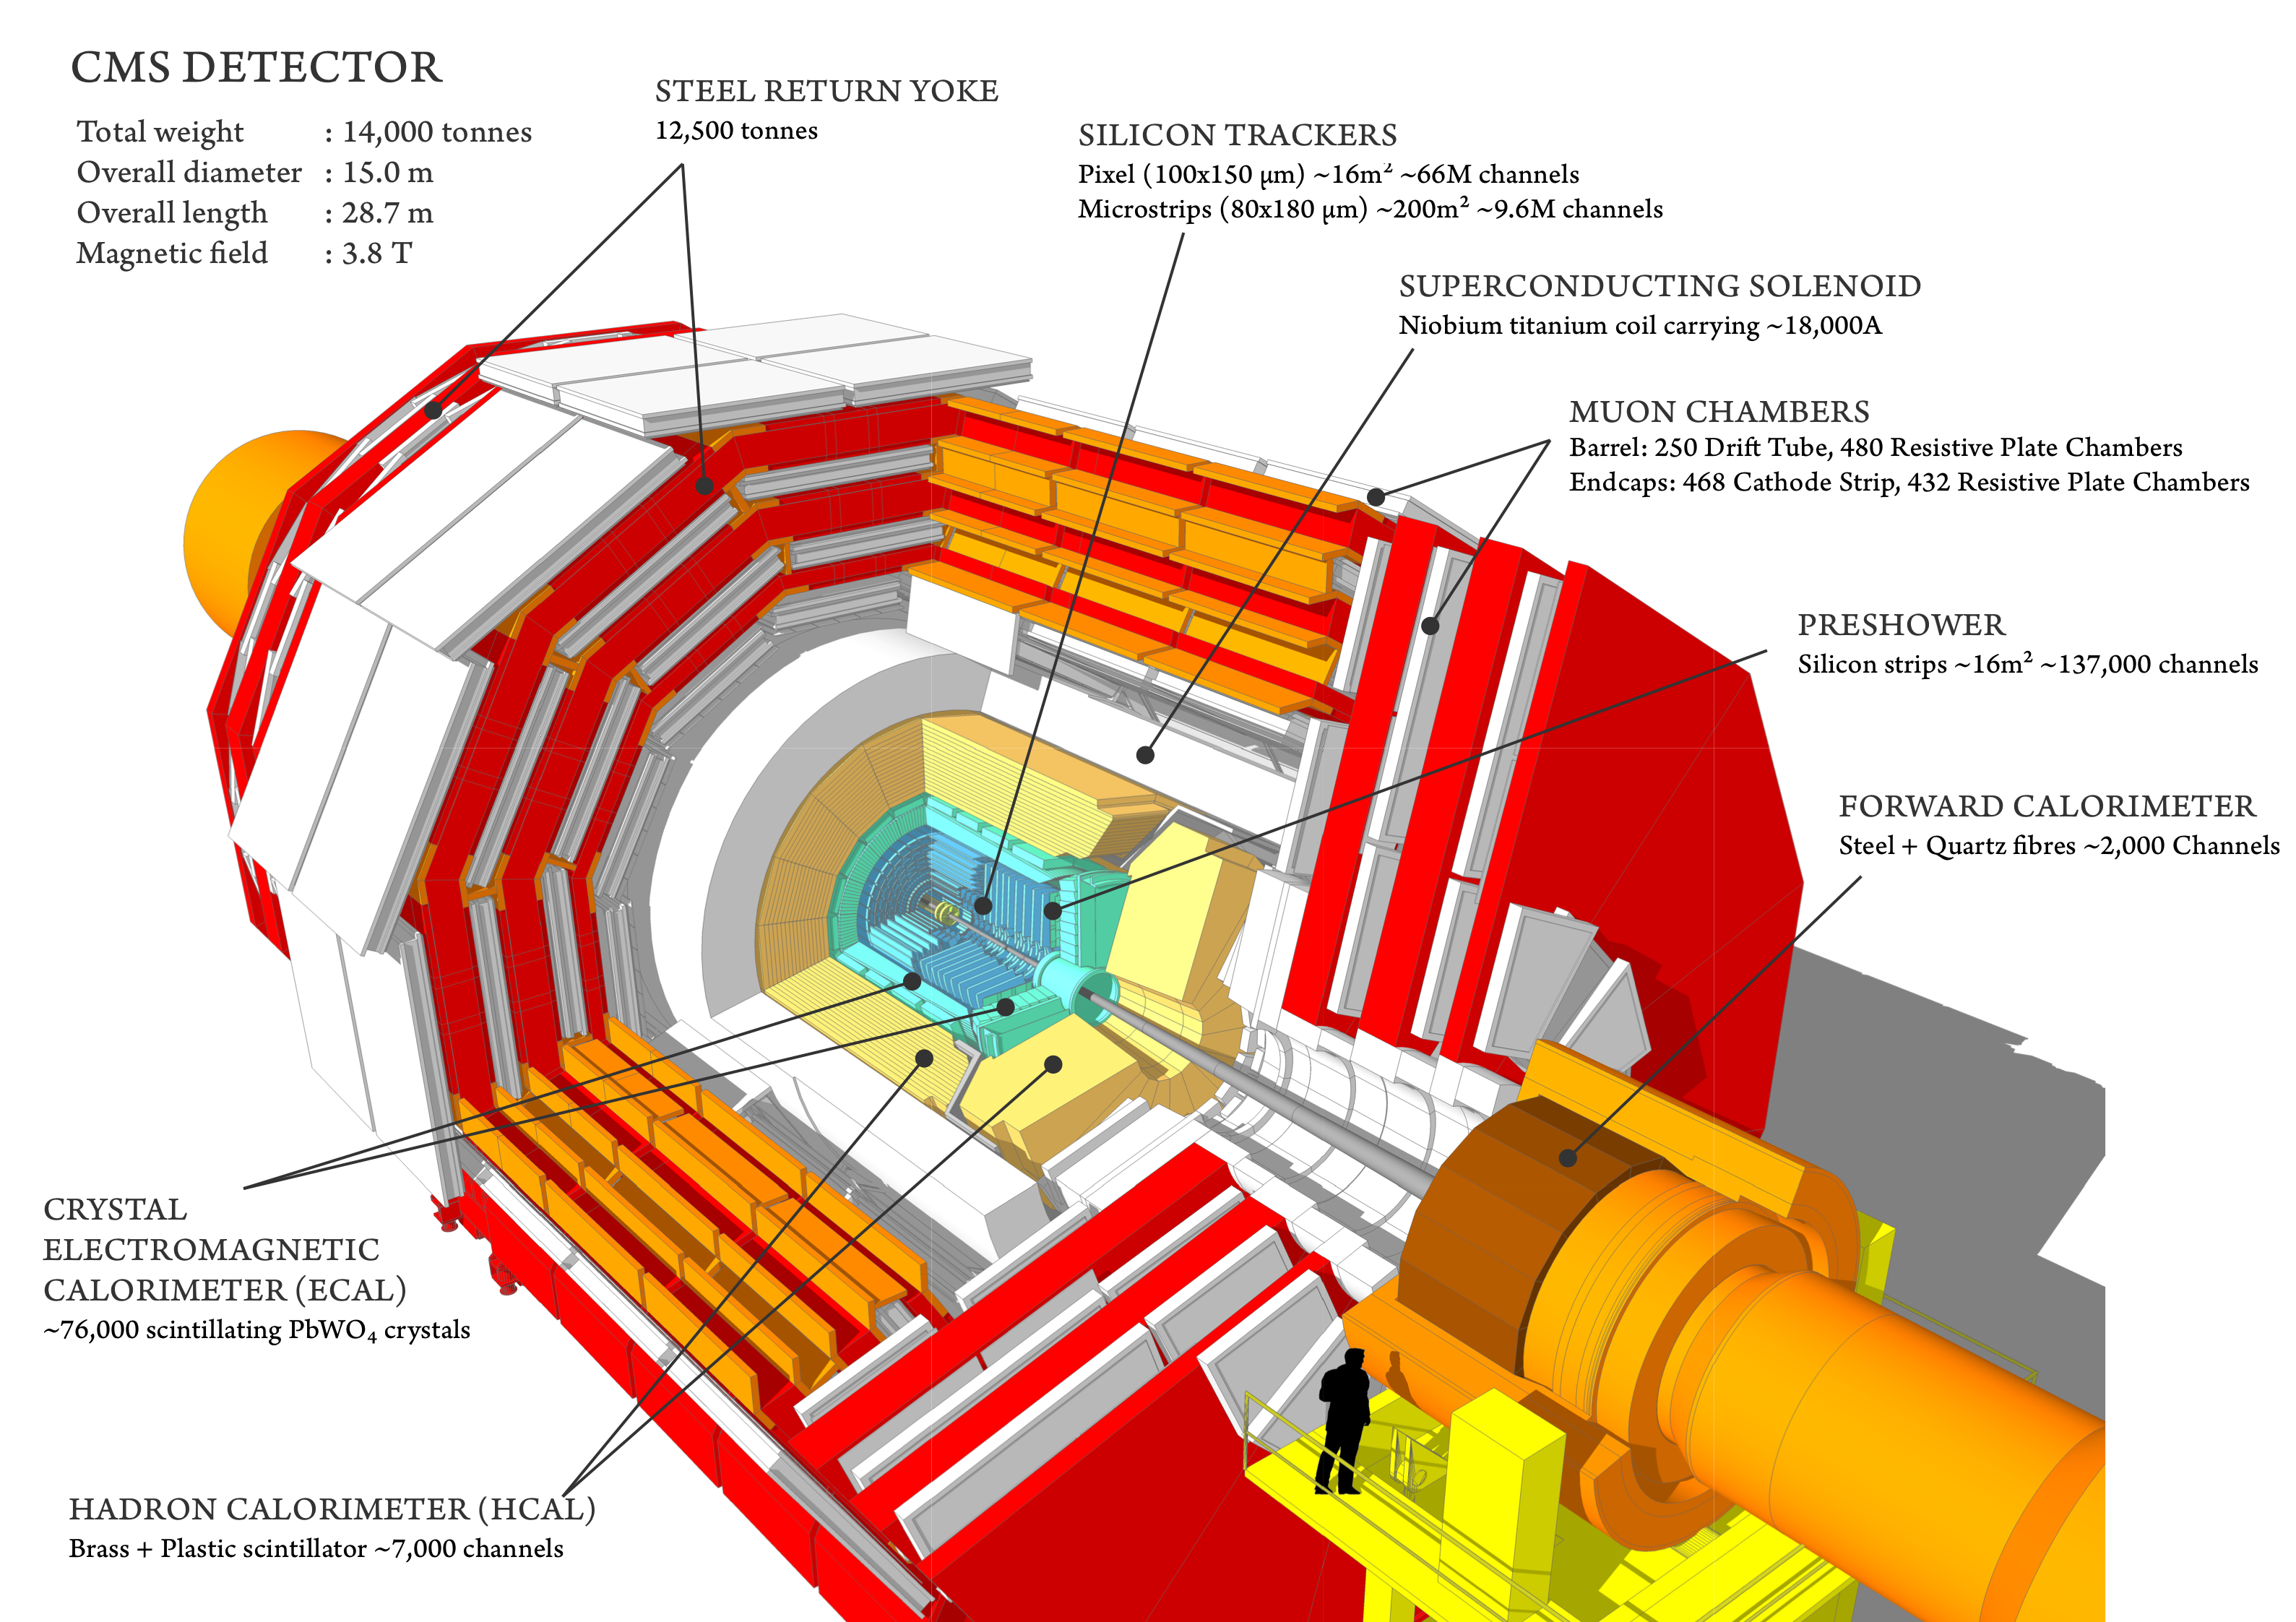
\includegraphics[width=0.8\textwidth]{ch2_cms_exp/plots/cms_diagram.png}
  \caption[CMS diagram]{This is a schematic representation of \ac{cms}}
  \label{fig:cms_diagram}
\end{figure}

\subsection{Tracking system}



\subsection{ECAL}

\subsubsection{Material description}

\subsubsection{Photon reconstruction}
- super cluster algorithm
- differences between photons and electrons (hence why so good for comparisons because can ignore the electron track)

\subsubsection{Photon corrections}
- photon resolution formula
- transparency corrections
- crack corrections etc. (superseding by regression)

\subsection{HCAL}

\subsection{Muons}

\subsection{Isolation and particle flow}






  \chapter{Common analysis components}
\label{chap:common_analysis_components}
\chapterquote{I don't have a quote}
{Matthew Kenzie, 1785--1854}

This thesis describes three complementary analysis regimes in the Higgs to two photons search at CMS. These differ in their photon selection, event selection, event classification (or categorisation) and statistical methods for extracting results. They are described in the following chapter (Chapter~\ref{chap:selection_and_categorisation}). However, there are many components which they share. These are detailed below.

As we have seen in Eq.~\ref{eq:invmass}, repeated below in Eq.~\ref{eq:invmass2} for convenience, the diphoton invariant mass is constructed from the two photon energies and the angle between them. Consequently, important considerations for this analysis are photon energy resolution and good opening angle resolution which is completely dominated by the vertex resolution, as the position resolution of the photons (location they hit the \ECAL) is neglible in comparison. Details of how this is exploited in the analyses are given at the end of this chapter in Sections~\ref{sec:photon_energy} and~\ref{sec:vtx_reco}. The selection of events is described in the chapter after this (Chapter~\ref{chap:selection_and_categorisation}) alongside the categorisation, or binning, scheme into different classes of event which take advantage of areas of phase space which share similar signal to background ratios.

\begin{equation}
  m_{\gamma\gamma} = \sqrt{E_{1}E_{2}(1-\cos(\alpha))}
  \label{eq:invmass2}
\end{equation}

After a preliminary discussion of multivariate analysis techniques, the datasets, the triggering and the \MC are discussed.

\section{Boosted Decision Trees}
\label{sec:bdts}

\MVAs are commonly used in High Energy Physics analyses to extract the maximum possible signal sensitivity in cases where the background rates are high. The advantage of \MVAs is that given a set of input variables a network of sequential cuts can be built, to classify or correct events, in a multidimensional phase space to exploit differences between the signal and background in these variables and importantly in the correlations between these variables. A particular type of \MVA which is used widely in this analysis is the \BDT. \BDTs are prefered because they are more robust to the inclusion of variables which have little or no discriminating power. There are two broad types of \BDT used, one is known as a regression \BDT and the other as a classification \BDT. 

A classification \BDT will, given a set of input variables, assign a value (typically between -1 and 1) to each event based on how signal like that event is. This serves to collapse all the event information into one discrimanting variable which can be used to classify differences between the signal and background. The input is provided as the probability distributions (which can be supplied as binned or unbinned data samples or as a functional form) of the background and signal for a set of ``input variables". The process involves construction of a series of \DTs complemented by a ``boosting" step which serves to mitigate against ``overtraining" on fluctuations within the training samples. This analysis chooses a particular type of decision tree boosting known as ``gradient" boosting because it is more robust against outliers or mislabled data points~\cite{TMVA}.

The \DT is built by applying sequential cuts to the input variables and assessing the relative signal purity, $p$, in the sub-sample remaining after each cut.

\begin{equation}
  p = \frac{N_{s}}{N_{s}+N_{b}},
\end{equation}

where $N_{s}$ and $N_{b}$ are the sum of weights of the signal and background remaining in each sub-sample. A threshold criterion, known as the Gini index~\cite{TMVA} $p(1-p)$, is applied to decide whether to split the sample further. The process continues and the splitting is curtailed when either the threshold or the user defined maximum tree depth (number of subsamples allowed) is reached. The value of each cut is varied such that the signal purity, $p$, in each sub-sample is maximised. An event is assigned a value of -1 or +1 depending on whether it falls into a sub-sample with $p>$0.5 or not. Clearly some fraction of events will be misclassifed where the actual number which get misclassified will depend on the discrimnatory power available from the chosen input variables. In order to reduce this effect a series of \DTs are trained and each assigned a weight derived by the ``boosting" process. 
If we assign each \DT as a member of a family of $M$ functions, $f(\vec{x};\vec{a}_{m})$, which depend on the input variables, $\vec{x}$ and the set of cuts in that tree, $\vec{a}_{m}$. The object is to construct an overall decision tree which consists of the weighted average of each \DT,

\begin{equation}
  F(\vec{x};\vec{\beta},\vec{a}) = \sum_{m=0}^{M} \beta_{m}f(\vec{x},\vec{a}_{m}) \;\;\;\;\; \textrm{where} \;\; \vec{\beta} = (\beta_{0},\beta_{1}...\beta_{m})
\end{equation}

The boosting procedue is implemented by adjusting the weights $\vec{\beta}$ in order to minimise the deviation in the loss function (Eq.~\ref{eq:bdt_loss_fcn}) between the weighted tree response $F(\vec{x};\vec{\beta},\vec{a})$ and the true output $y$ obtained from the training sample. 

\begin{equation}
  L(F,y) = \ln(1+e^{-2F(x)y})
  \label{eq:bdt_loss_fcn}
\end{equation}

A common procedure when constructing a \BDT to check for overtraining is to split both the background and signal into two independent samples. One is used to \emph{train} the \BDT and one is used to \emph{test} the response of the output. Clearly one requires that both the training and independent test sample look the same in the output variable. This is usually quantified by use of a Kolmogorov-Smirnov test, which broadly speaking ascertains the probability that the training and test samples originate from the same underlying distribution~\cite{kol_smir}. 

In this way the output of $F(\vec{x};\vec{\beta},\vec{a})$ for a classification \BDT will be a ``semi-continuous" output from -1 to 1 with signal events in general given a higher score than background events.

A regression \BDT is used to estimate the true value of some variable given the values and correlations of several other variables. They are commonly used for correcting the energy of a particular object, for example a photon. Given a \MC source of photons the ``true" energy is regressed from the position, shape and raw energy of the supercluster. For regression \BDTs the output $F(\vec{x};\vec{\beta},\vec{a})$ represents the estimated corrected energy and the boosting procedure targets minimising the deviation between this and the true energy in \MC. 

\section{Data samples and triggering}

The data consists of two indepedent samples of proton-proton collisions collected by the CMS experiment at the \LHC in 2011 and 2012 with a centre-of-mass energy ($\sqrt{s}$) of 7 and 8 TeV respecivtely. The total integrated luminosity of the two samples is 5.1\fb and 19.7\fb in 2011 and 2012 respectively and collectively referred to as \LHC Run 1. The response of the detector has changed considerably over this period and much of the variation is modelled by the \MC simulation. Figure~\ref{fig:intlumi} shows the integrated luminosity delivered and recorded by \CMS during \LHC Run 1.

\begin{figure}
  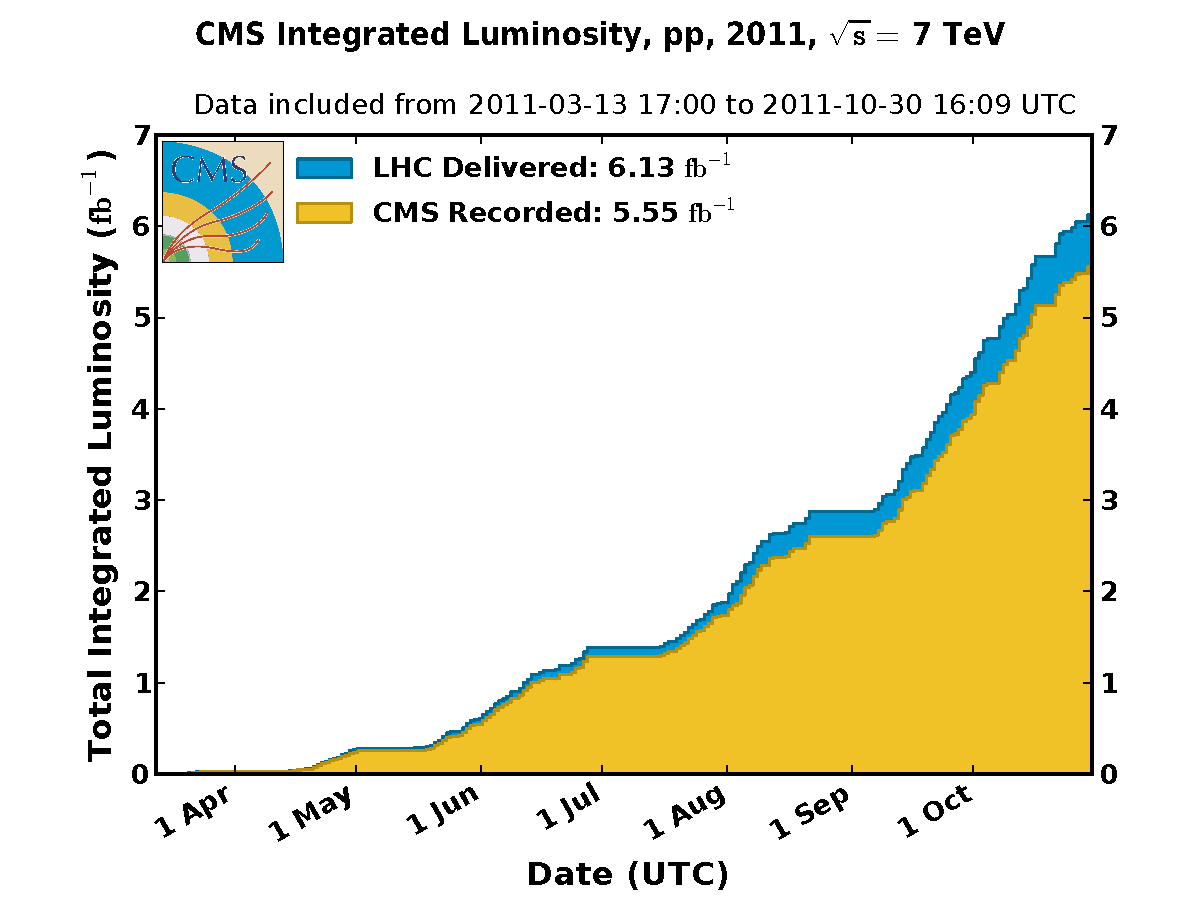
\includegraphics[width=0.49\textwidth]{ch3_comm_anal_comps/plots/int_lumi_2011.pdf}
  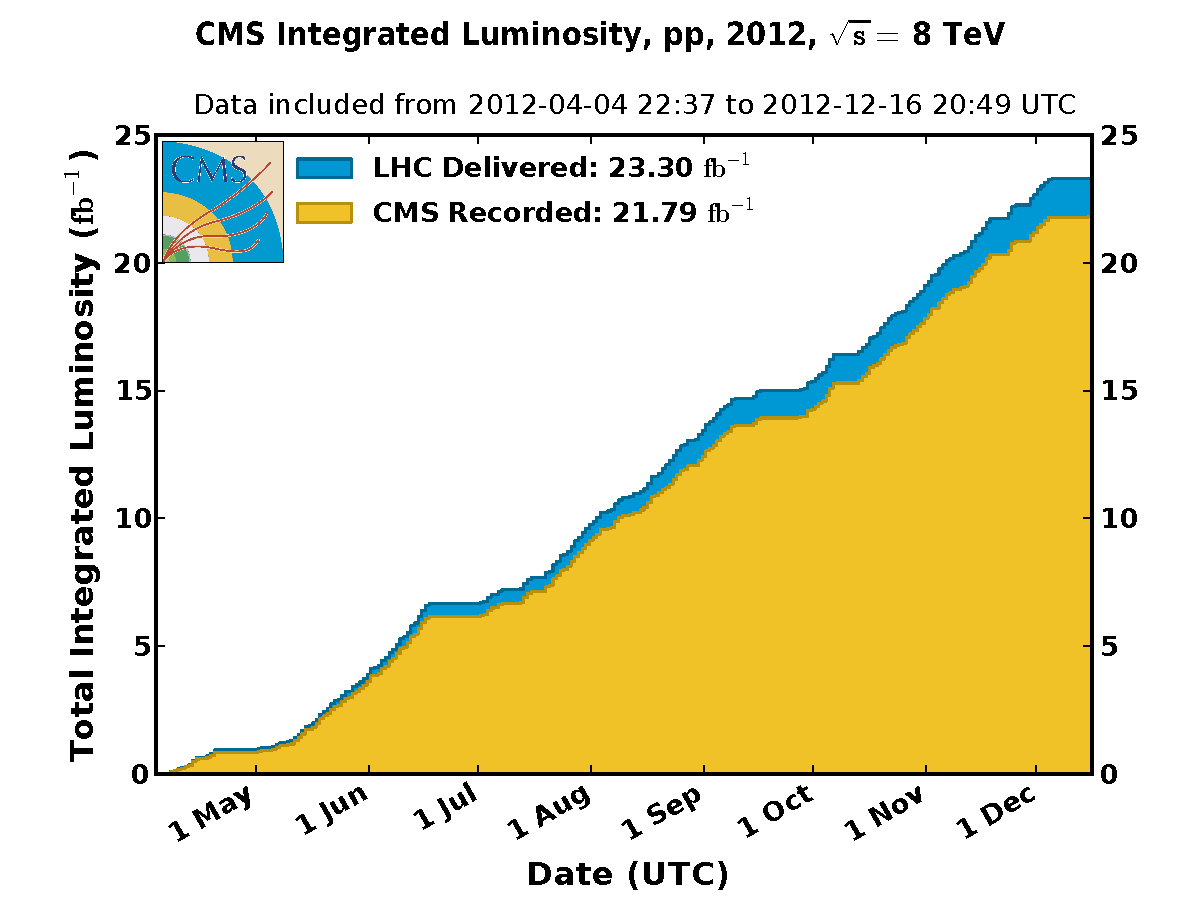
\includegraphics[width=0.49\textwidth]{ch3_comm_anal_comps/plots/int_lumi_2012.pdf}
  \caption{The total integrated luminosity delived and recorded by CMS during the 2011 (left) and 2012 (right) run periods.}
  \label{fig:intlumi}
\end{figure}

Events are selected for the analysis by requiring they pass an asymmetric diphoton trigger with \ET thresholds of 26 (18) and 36 (22) GeV for the leading (trailing) photon in the 2011 and 2012 runs respectively. The candidates are also required to have either a high value of \rnine or to pass a loose calorimetric identifaction and isolation requirement. High trigger efficiency is achieved by selecting photon candidates which pass either requirement. The efficiency of the trigger for the analysis preselection is 99.5\%.

\subsection{Monte Carlo}
\label{sec:mc}

Accurate simulation of detector effects and efficiency is highly important. Knowledge of the expected Higgs signal shape is clearly essential and although the size and shape of the \mgg background is entirely data driven when extracting results, simultaing the kinematics, shower shape and resolution properties of the background is essential when training the selection and optimising the binning. 

As explained in Chapter~\ref{chap:intro} the two main production mechanisms for a \SM Higgs boson at the \LHC are \ggH and \VBF. Typically the latter is produced at much higher Higgs \pT and this feature is exploited in the analysis. Consequently, it is important to model the \pT distribution of these two production modes accurately. The signal samples for these two processes are generated using \POWHEG~\cite{powheg1,powheg2} at NLO interfaced with \PYTHIA~\cite{pythia} including a reweighting factor which matches their \pT spectrum to that when including the NNLO and NNLL terms. For the associated production modes, with a $W^{\pm}$,$Z$ or $t$-quarks, (\VH and \ttH) only \PYTHIA is used. The \SM Higgs boson cross sections and branching fractions are taken from Ref.~\cite{LHCHiggsCrossSectionWorkingGroup3}

The spin-2 graviton with minimal couplings, \graviton, has two production mechanisms, one via gluon-fusion ($ggX$) and one via quark-antiquark annihilation ($q\bar{q}X$). The graviton samples are generated using the \JHU generator~\cite{jhu} in which the \pT spectrum of these samples is matched to the SM so that any bias obtained from mismodelling of the $\pT$ is avoided.

The simulated background samples are used soley for cut and category optimisations and training of multivariate discriminants. The background which contains the \QCD continuum of prompt photons (refering back to Chapter~\ref{chap:intro} these are produced by Born and Box diagrams) is simulated using \SHERPA~\cite{sherpa} at 8\TeV and \MADGRAPH~\cite{madgraph} at 7\TeV. The prompt-fake and fake-fake backgrounds, in which one or more photons are faked by a neutral meson (usually a \pizero) reconstructed as a jet are generated using \PYTHIA. Samples of \Zee, \Zmumu and \Zmumugamma used for data/MC comparisons are generated with \POWHEG.

All of these \emph{generator level} samples are then run through the full \CMS detector simulation using \GEANT~\cite{geant}. This includes the effect of overlapping vertices (pileup) and detector effects (such as noise and crystal degredation) in four bins of time (Run2011, Run2012AB, Run2012C, Run2012D).


\subsection{Pileup and beamspot reweighting}
\label{sec:pileup_beamspot}

An important difference between the simulated samples and the data which can have a large impact on the analysis is the distribution of the number of primary vertices. The \emph{pileup} in the event effects many important analysis variables, for example photon shower shape and photon isolation as well as the diphoton invariant mass if the chosen vertex is wrong. Consequently the \MC is reweighted such that the pileup distribution matches that in data. The reweighting technique is validated using \Zmumu events as shown in Figure~\ref{fig:pileup} for the 7 and 8~\TeV samples respectively. 

\begin{figure}
  \begin{center}
  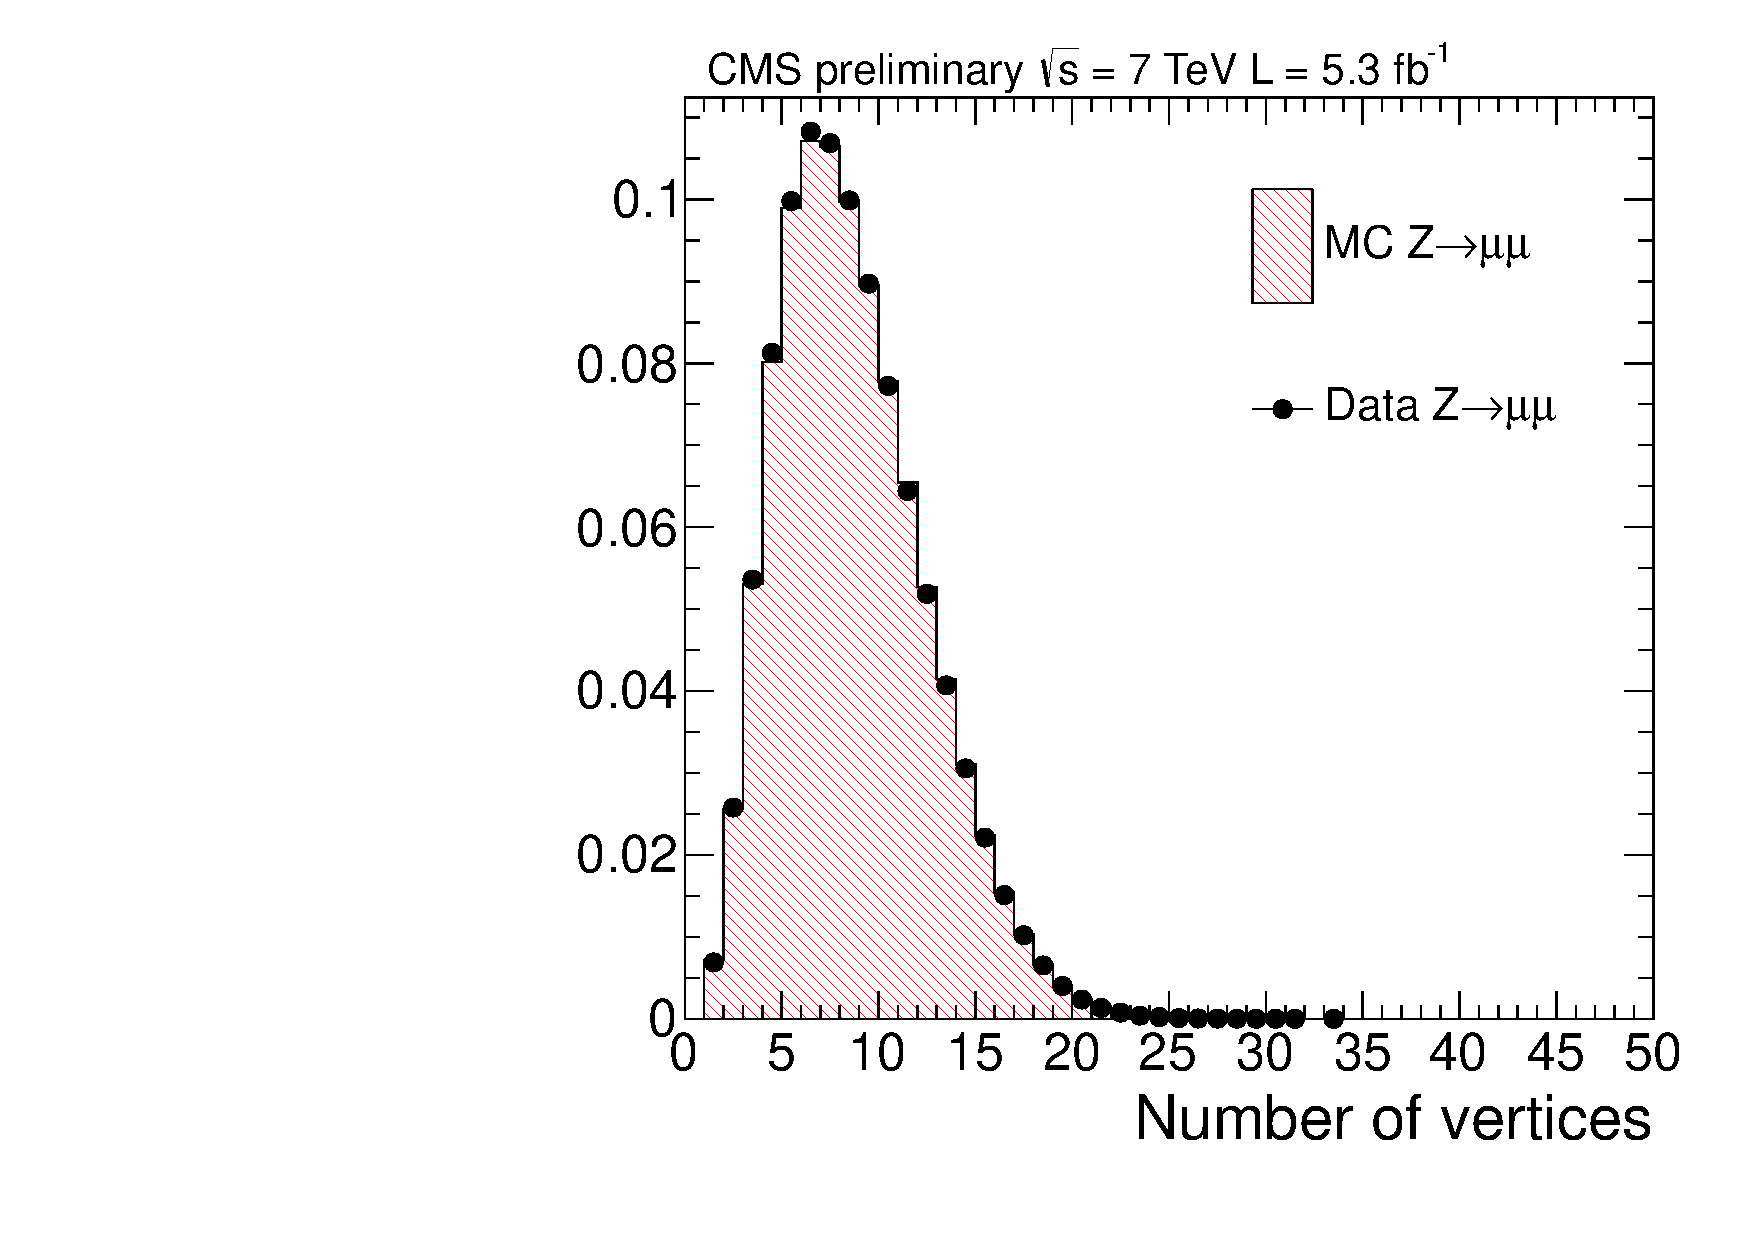
\includegraphics[width=0.49\textwidth]{ch3_comm_anal_comps/plots/nvtx_zmumu_2011.pdf}
  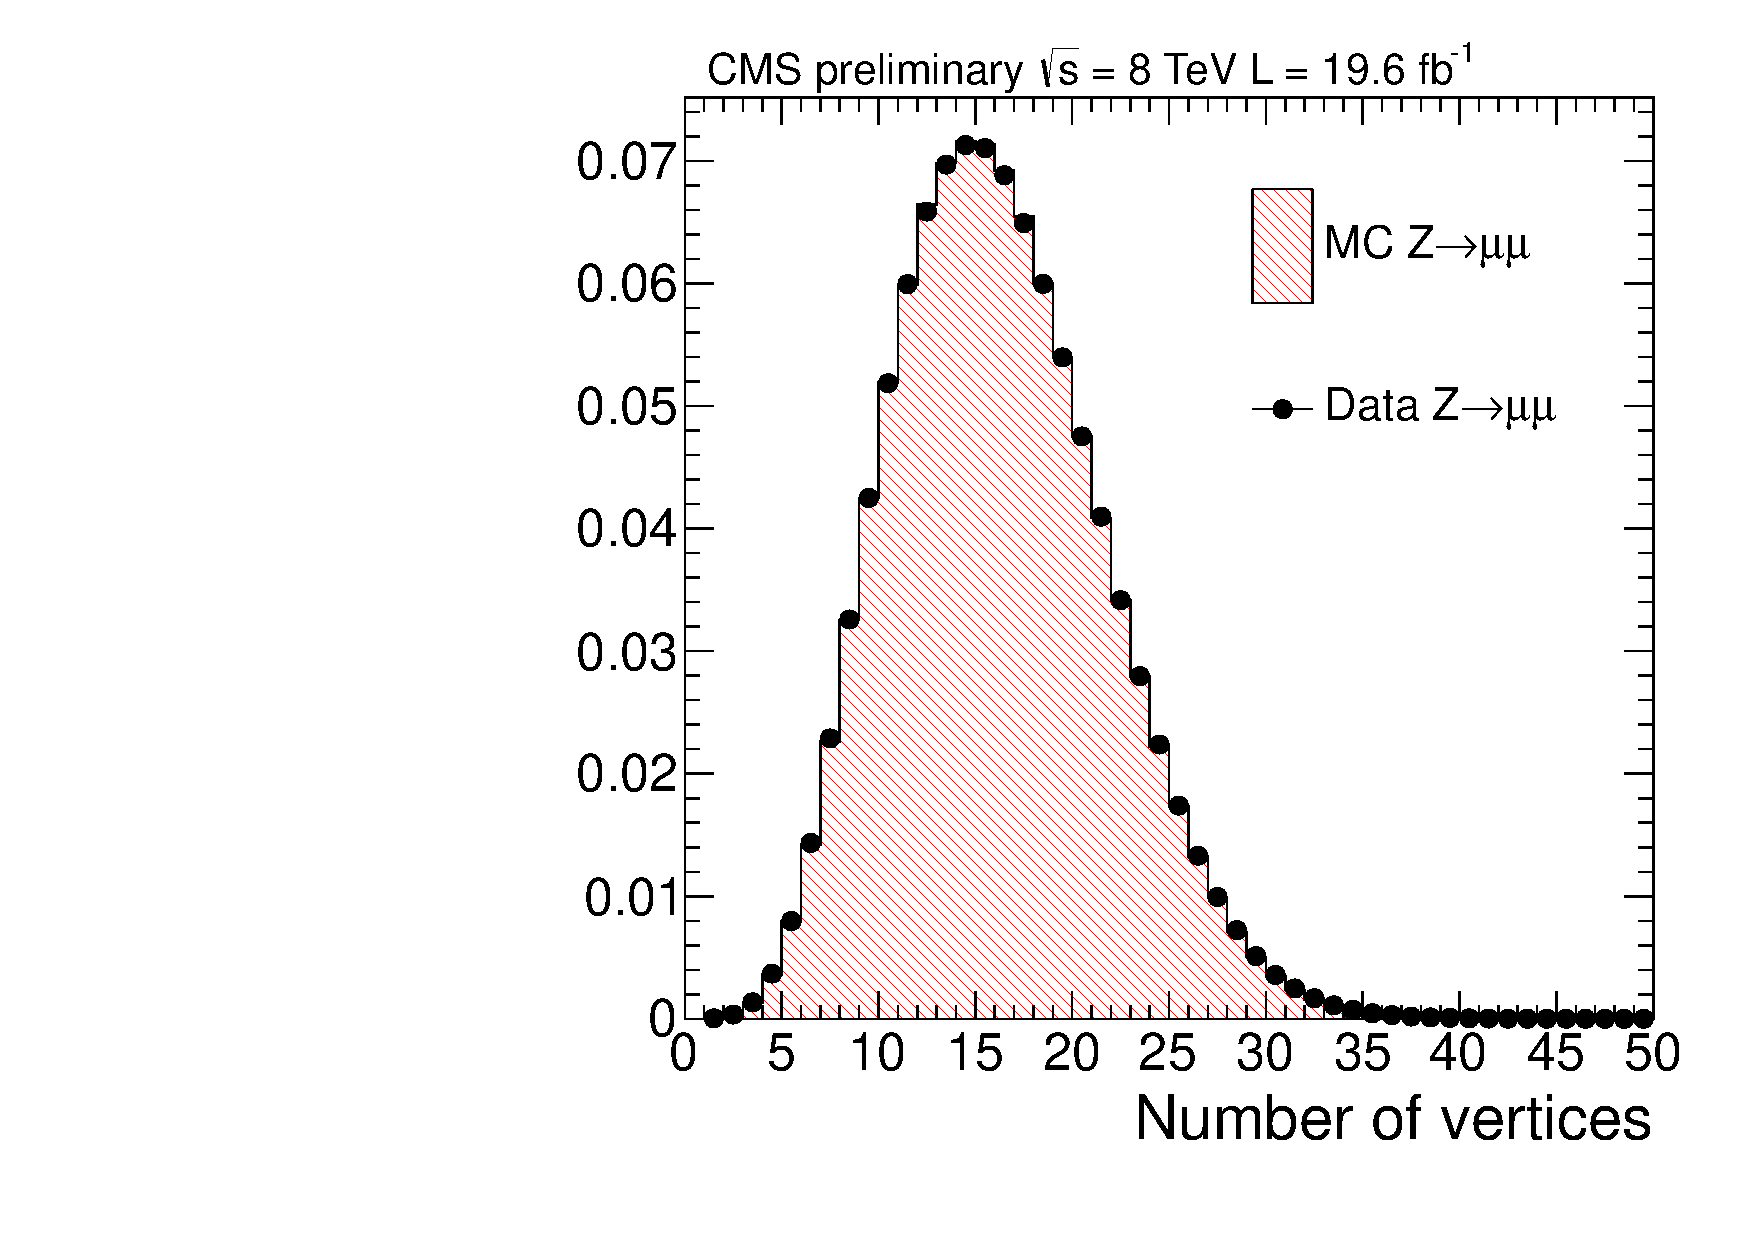
\includegraphics[width=0.49\textwidth]{ch3_comm_anal_comps/plots/nvtx_zmumu_2012.pdf}
  \caption{Distribution of the number of reconstructed vertices in the 2011 (left) and 2012 (right) run periods. Calculated using the Deterministic Annealing alogirithm in \refrqd for \Zmumu events in data (black dots) and MC (red histogram) after reweighting.}
  \label{fig:pileup}
  \end{center}
\end{figure}

When the chosen vertex is incorrect the mass resolution is dominated by the spread in position of the pileup vertices (known as the beamspot width, $\sigma_{z}^{beamspot}$). Accurate modelling of this spread is important so that the resolution of wrong vertex events in simulation matches that in data. The \MC overestimates the beamspot spread by some 20\% so a simple reweighting is implemented for \MC events in which the wrong vertex chosen (as the effect is neglible for events in which the chosen vertex is correct) such that the distribution of the distance between the chosen vertex postion and the true vertex position, $\delta z=z_{chosen}-z_{true}$, match between data and \MC. The effect with and without reweighting compared to data is shown in Figure~\ref{fig:beamspot}.

\begin{figure}
  \begin{center}
  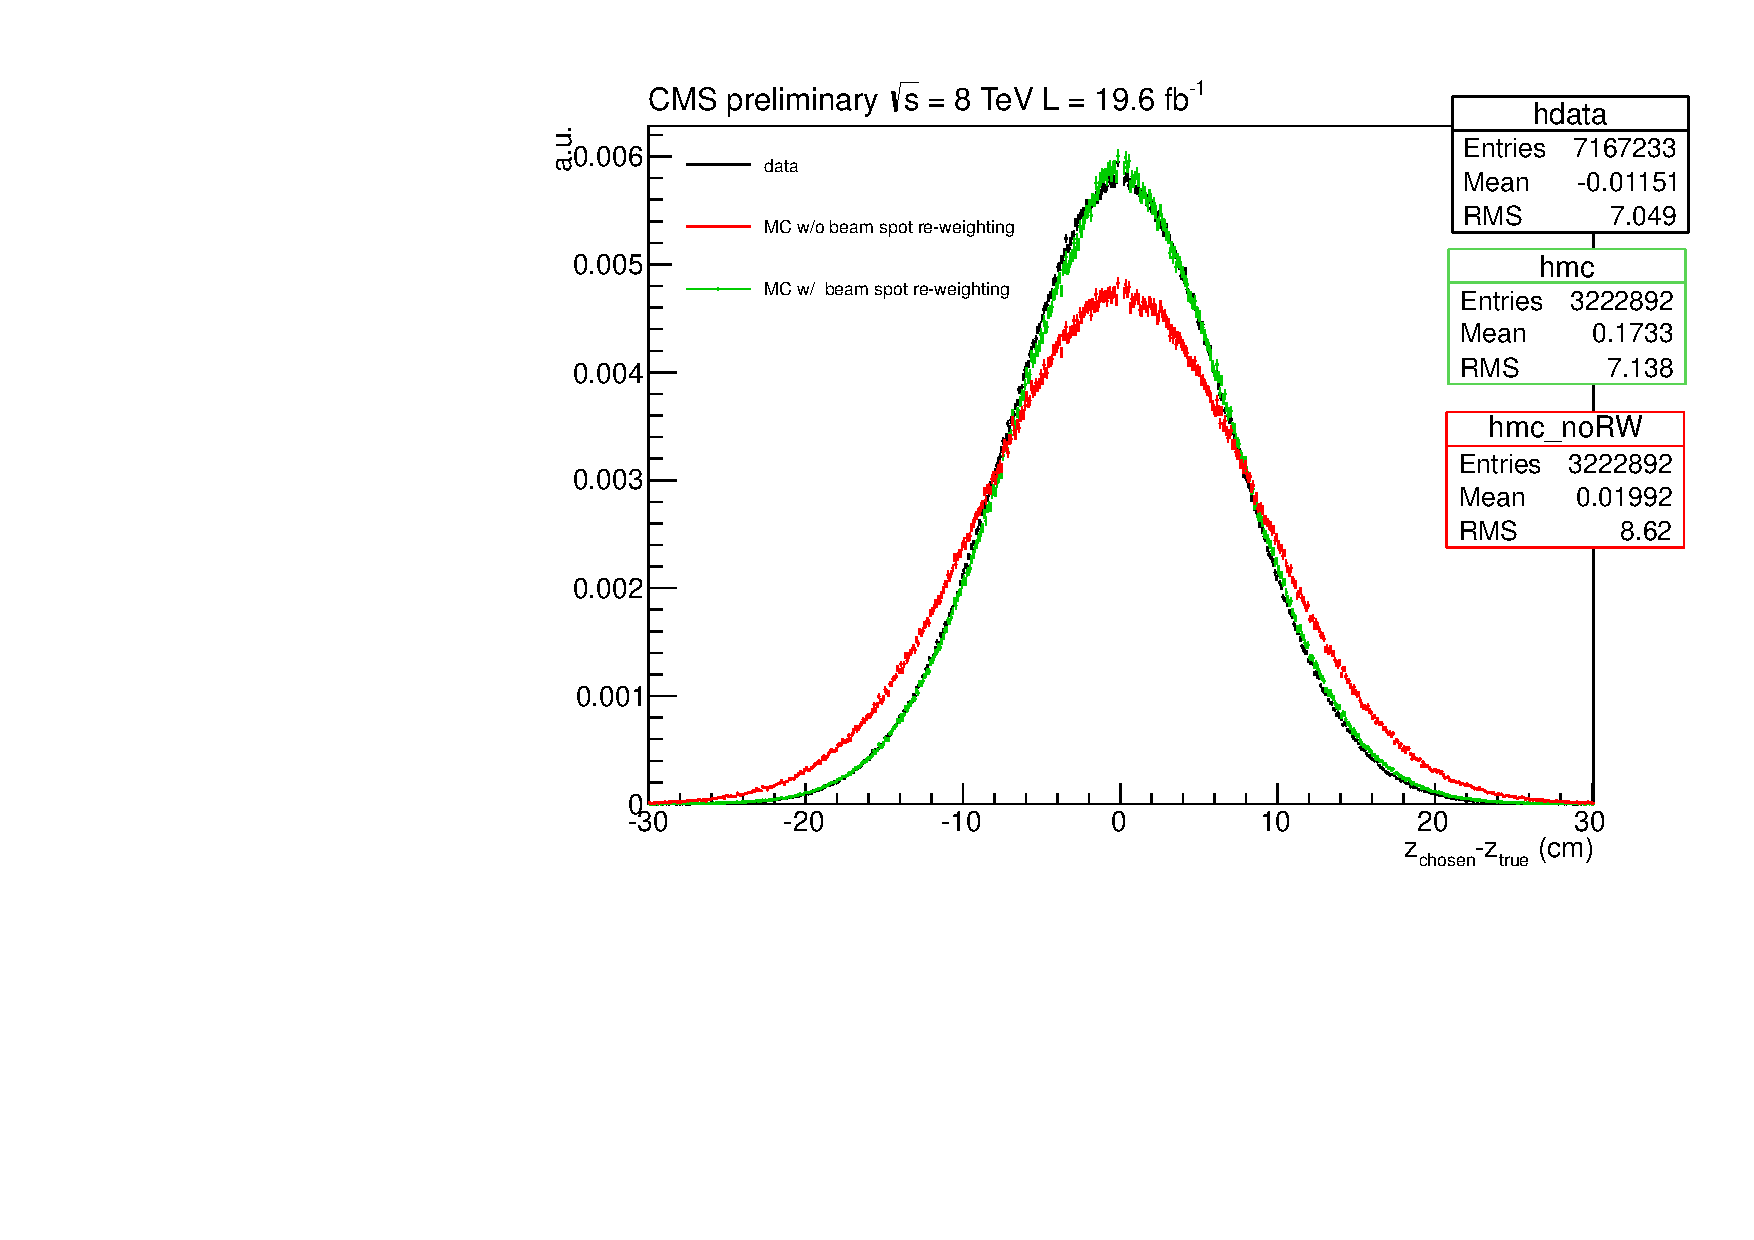
\includegraphics[width=0.55\textwidth]{ch3_comm_anal_comps/plots/beamspot.pdf}
  \caption{Distribution of $\Delta z$ (the distance between the chosen vertex and the true vertex in the $z$ direction) for data (black), the \MC (red) and the \MC after beam spot reweighting (green) for \Zmumu events.}
  \label{fig:beamspot}
  \end{center}
\end{figure}

\section{Energy measurement of photons}
\label{sec:photon_energy}

The photon energy obtained from the supercluster sum described in Section~\ref{sec:ecal} even when including the intercalibration and transperency corrections shown in Figure~\ref{fig:ecal_laser_corrs} does not give the most optimal resolution for the energy measurement of photons at \CMS. On top of this energy (known as the \emph{raw} supercluster energy, $E_{raw}$) it is also valuable to correct for additional energy losses. These arise from \emph{bremstrauhlung}; where the photon converts in the material upstream of the \ECAL and the two electron legs radiate additional photons and thus the some of the photon shower is missed, and for local containment of the shower; where some energy is lost through small gaps between \ECAL crystals and larger gaps between ``modules" or sections of crystals. These corrections are obtained using a specialised regression \BDT (see Sec.~\ref{sec:bdts}) trained on a \MC source of prompt photons from a sample containing photons and jets. The \BDT targets accurate measurements of individual photons' energy by correcting the raw supercluster energy and provides an estimate for the energy resolution of each photon given the position and shower shape of the supercluster. The training is done separately for barrel and endcap photons (as the cluster shapes look very different for these two distinct regions) and is also performed separately for the 7 and 8 TeV datasets. The following input variables are used:

\begin{itemize}
  \item The global position of the supercluster in \eta and \phi
  \item A collection of shower shape variables which aim at providing information on the likelihood and location of a photon conversion and the degree of showering in the material:
  \begin{itemize}
    \item The \rnine of the supercluster (as previously described in Section~\ref{sec:ecal}).
    \item The ratio of the 5$\times$5 crystal energy to the raw supercluster energy (equivalent of $R_{25}$).
    \item The energy weighted \eta-width and \phi-width of the supercluster (in other words the spread of the shower).
    \item The number of basic clusters.
    \item The ratio of energy in the \HCAL behind the supercluster to the \ECAL energy of the supercluster, $H/E$.
    \item The ratio of the preshower energy to the raw supercluster energy (endcap only).
  \end{itemize}
  \item A collection of the seed crystal and the seed cluster variables which aim at providing information about energy lost through gaps and cracks between crystal and crystal modules:
  \begin{itemize}
    \item The relative energy and position of the seed cluster.
    \item The local energy covariance matrix.
    \item Energy ratios between the seed and the 3$\times$3 and 5$\times$5 areas around the seed.
    \item The \eta and \phi index of the seed crystal and the relative position of the seed cluster to the crystal centre. 
  \end{itemize}
  \item Additionally the number of primary vertices and the median energy density, \rho, (see Sec.~\ref{sec:pileup}) are included to account for residual energy scale effects from pileup.
\end{itemize}

The regression is trained using an additional piece to that described in Section~\ref{sec:bdts} whereby the target is to predict the full probability distribution of the ratio of the true energy to the raw energy, $E_{true}/E_{raw}$. The target is a double crystal ball distribution which consists of a Gaussian core and power law tails on either side. This can be fully parametrised by six variables, the Gaussian mean and width ($\mu$, $\sigma$), the power parameters ($n_{L}$, $n_{R}$) and the power law tail cutoff parameters ($\alpha_{L}$, $\alpha_{R}$). Each of these parameters has a non-parametric dependence on the input variables, $\vec{x}$, and this is \emph{learned} by the regression training whilst simultaneously minimising the likelihood,

\begin{equation}
  -\ln \mathcal{L} = - \sum_{MC photons} \ln p(E_{true}/E_{raw} | \mu(\vec{x}),\sigma(\vec{x}),\alpha_{L}(\vec{x}),\alpha_{R}(\vec{x}),n_{L}(\vec{x}),n_{R}(\vec{x})),
\end{equation}

for the double crystal ball distribution, $p$. The most probable value for the true energy estimate of each photon is then given by,

\begin{equation}
  E(\vec{x},E_{raw}) = \mu(\vec{x})E_{raw}
\end{equation}

and the per-photon energy resolution is given by, 

\begin{equation}
  \frac{\sigma_{E}(\vec{x},E_{raw})}{E(\vec{x},E_{raw})} = \frac{\sigma(\vec{x})}{\mu(\vec{x})}.
\end{equation}

In this way the regression predicts the full probability density of $E_{true}/E_{raw}$ and provides an estimate of the optimal energy correction and the energy resolution per photon. A comparison of this distribution with a statistically independent \MC sample is shown for the 8~\TeV training in Figure~\ref{fig:regression_training}. The performance of the regression compared to the default photon reconstruction is shown in Figure~\ref{fig:regression_performance}.

\begin{figure}
  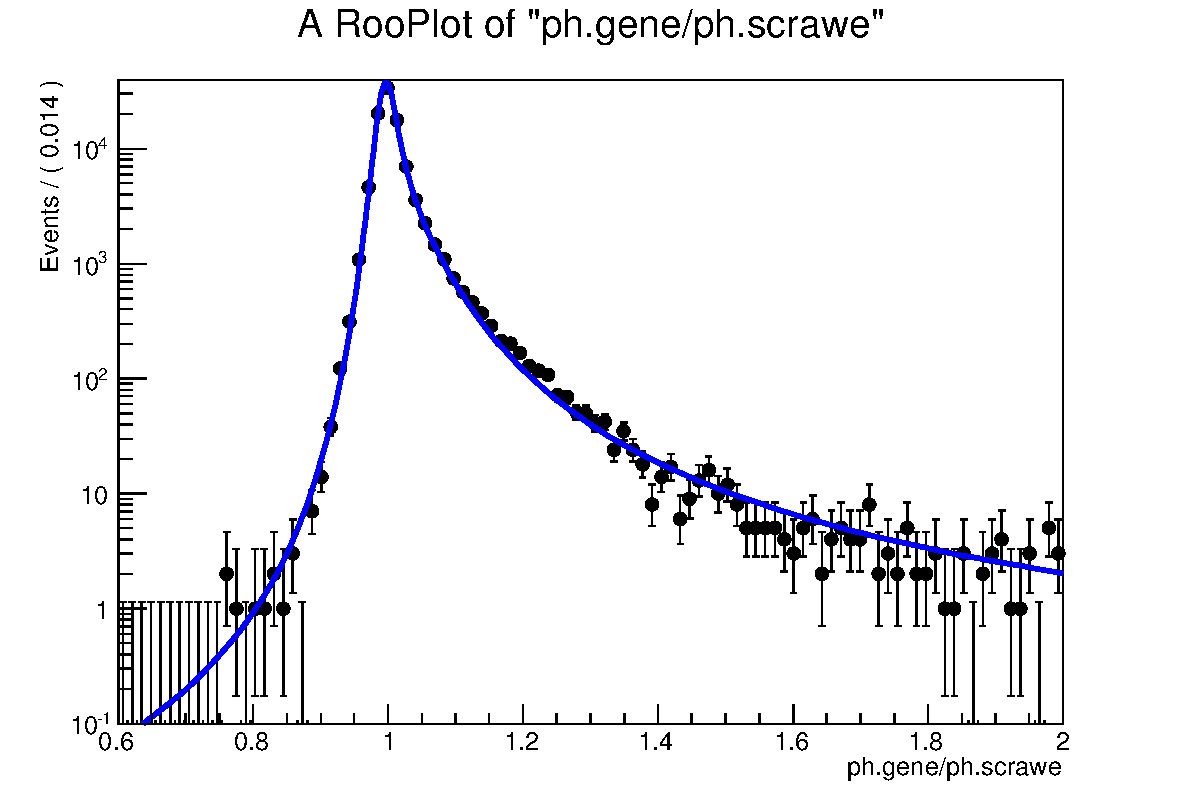
\includegraphics[width=0.48\textwidth]{ch3_comm_anal_comps/plots/regression_barrel.pdf}
  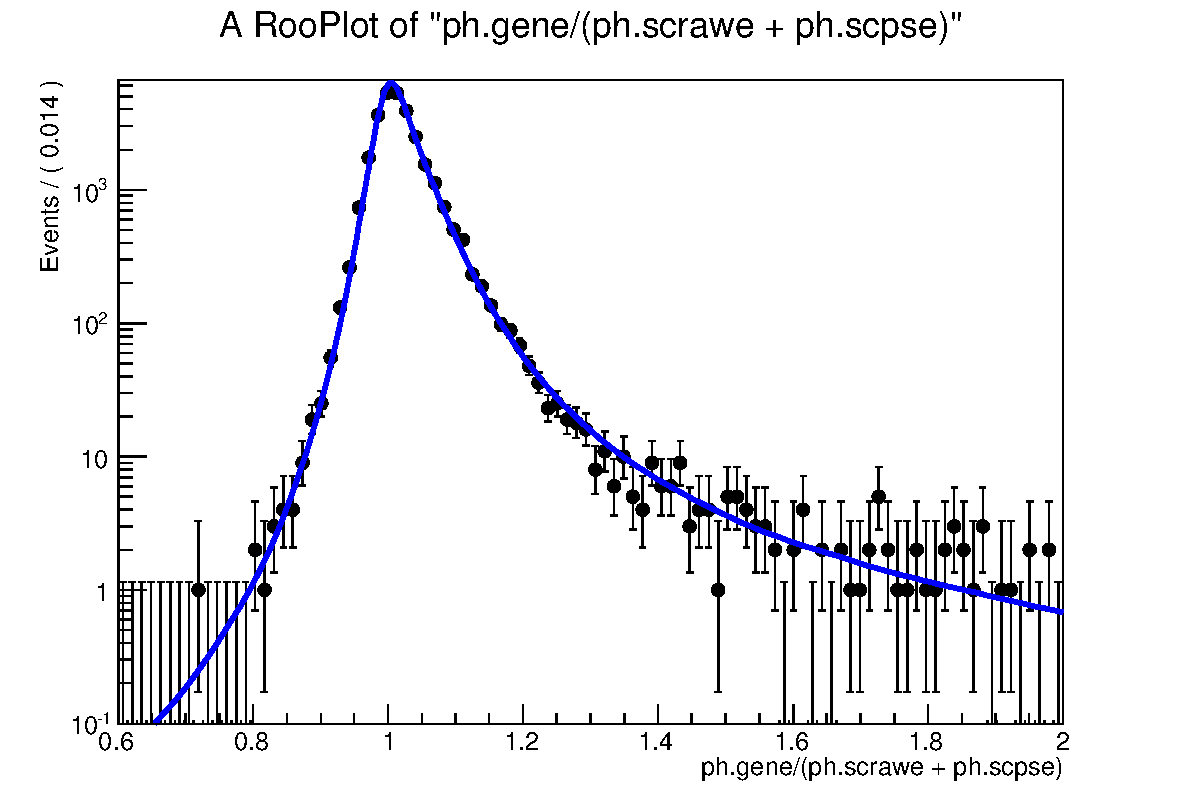
\includegraphics[width=0.48\textwidth]{ch3_comm_anal_comps/plots/regression_endcap.pdf}
  \caption{A comparison of the predicted probability density of $E_{true}/E_{raw}$ from the regression training (blue line) to the distribution in a statiscally independent \MC sample (black points) for barrel photons (left) and endcap photons (right). \red{PLOTS NEED TIDYING}}
  \label{fig:regression_training}
\end{figure}

\begin{figure}
  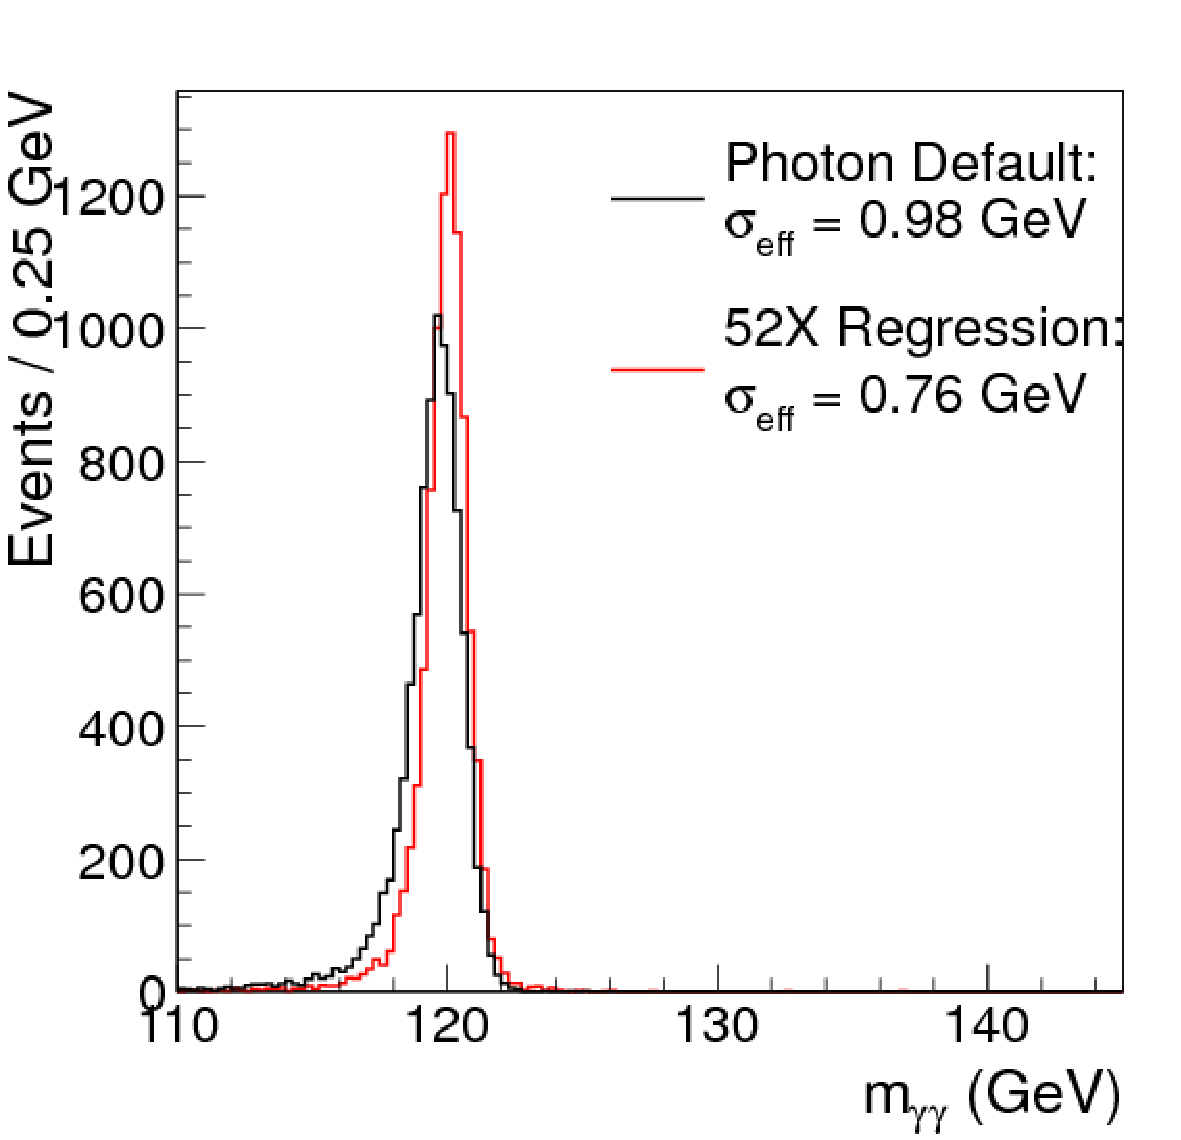
\includegraphics[width=0.24\textwidth]{ch3_comm_anal_comps/plots/regression_masscat0.pdf}
  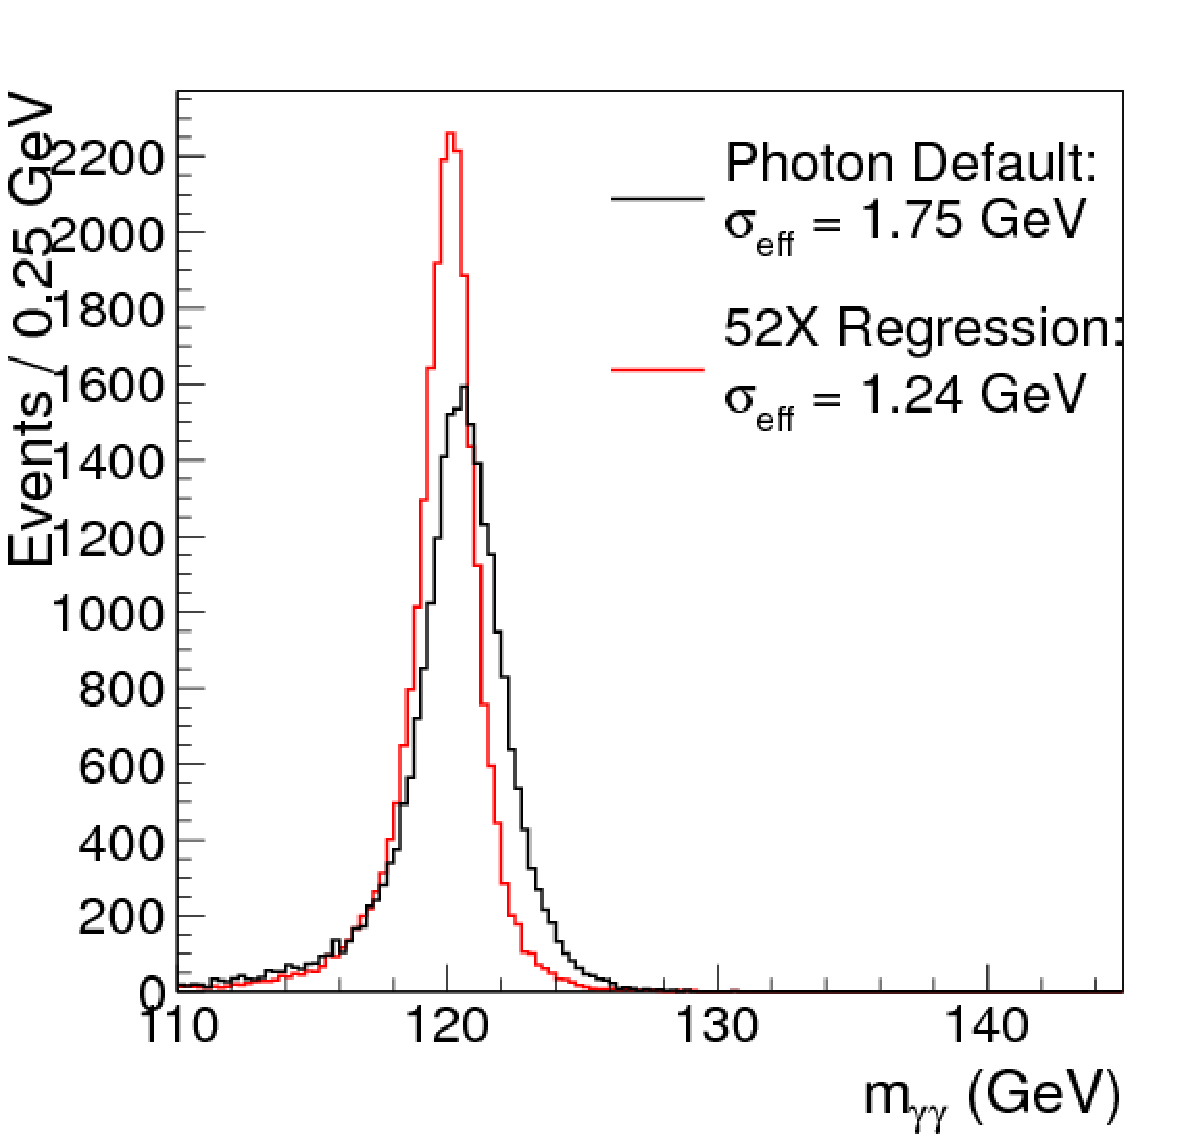
\includegraphics[width=0.24\textwidth]{ch3_comm_anal_comps/plots/regression_masscat1.pdf}
  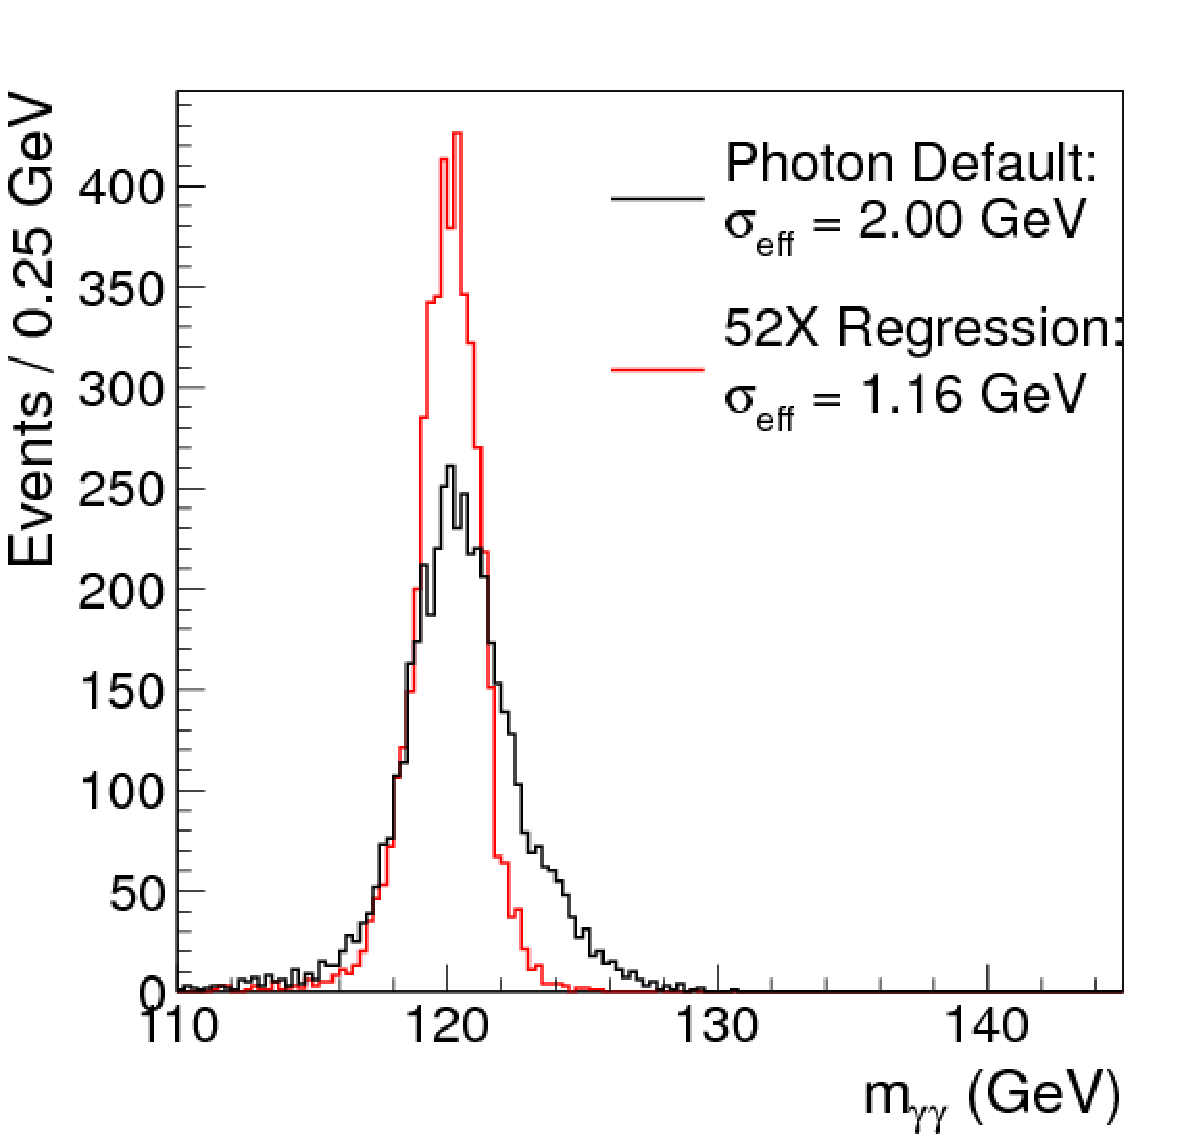
\includegraphics[width=0.24\textwidth]{ch3_comm_anal_comps/plots/regression_masscat2.pdf}
  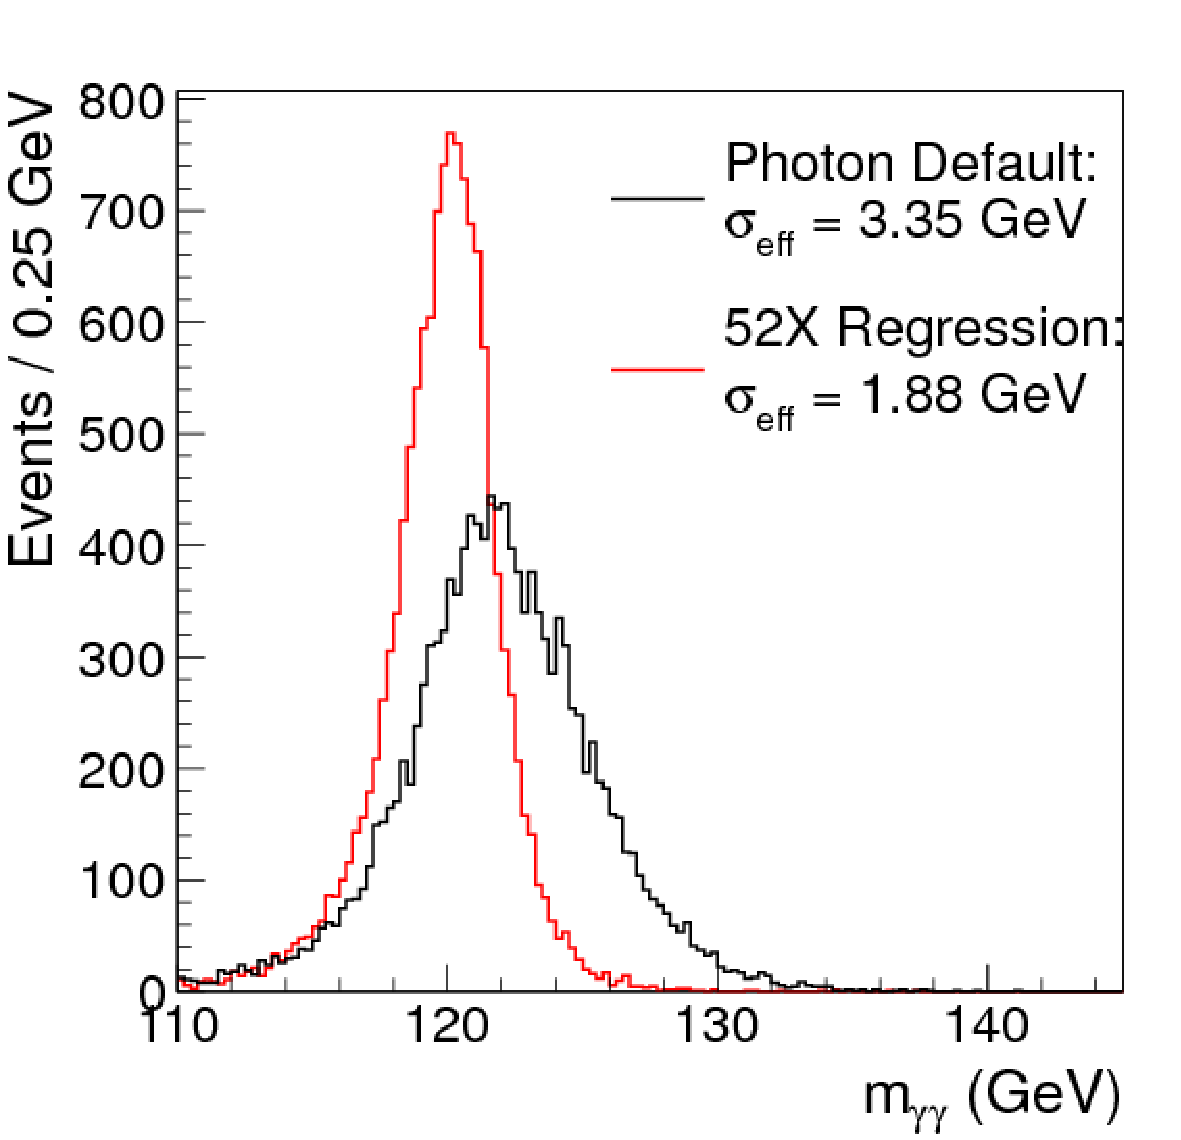
\includegraphics[width=0.24\textwidth]{ch3_comm_anal_comps/plots/regression_masscat3.pdf}
  \caption{A comparison of the regression performance compared to the photon default for the diphoton invariant mass on a \MC source of Higgs decays to two photons. This is shown when both photons are in the barrel (left two plots) when both photons have $\rnine>0.94$ (far left) and when at least one photon has $\rnine<0.94$ (middle left). When at least one photon is in the endcap (right two plots) when both photons have $\rnine>0.94$ (middle right) and when at least one photon has $\rnine<0.94$ (far right). The value shown in the legend of each is the effective width, $\sigma_{eff}$, which is defined as half of the narrowest interval which contains 68.3\% of the distribution. \red{PLOTS NEED TIDYING}.}
  \label{fig:regression_performance}
\end{figure}

\subsection{Correcting for residual discrepancies between data and Monte Carlo}
\label{sec:scale_smearing}

After application of the energy regression correction there are some remaining discrepancies between data and \MC. These residual effects are accounted for using \Zee events in data and simulation to correct the energy scale in the data and to apply an additional smearing term to the \MC with systematic uncertainties propagated through the analysis to account for the uncertainties on these corrections.

\subsubsection{Energy scale corrections to the data}

The supercluster energy is identical for electrons and photons so by correcting the supercluster energy scale to a known source, namely the mass of the $Z$-boson, in dielectron decays the smaller residual energy scale effects are accounted for. This can be done several times to account for various different effects. In the first stage scale corrections are derived in bins of time (run range) and \eta, after applying these corrections further, much smaller, residual effects are accounted for in bins of \rnine (the size of the effect is different for converted and non-converted photons). After applying both of these a further step is taken for the 8 TeV data in the barrel to derive residual corrections in bins of \ET. Consequently the total scale correction is a product of three corrections in 59 bins of time $\times$ 4 bins in \eta $\times$ 2 bins in \rnine $\times$ 6 bins in \ET (for the 8TeV barrel photons alone).

The strategy for deriving these corrections is to take \Zee events in data and \MC and extract the invariant dielectron mass in the relevant bin of interest. This mass distribution is fitted with a convolution of a Breit-Wigner (designed to handle the underlying Z line shape~\cite{pdg}) and a Crystal-Ball which models the calorimeter resolution effects and bremstrauhlung losses in the material upstream of the \ECAL. The Breit-Wigner parameters are fixed to the PDG values of $M_{Z}=91.188$~\GeV and $\Gamma_{Z}=2.495$~\GeV~\cite{pdg} whilst the Crystal-Ball parameters which model the detector effects are allowed to float. The scale correction, $\Delta E$, is then defined as the relative difference between the Crystal-Ball peak in data and simulation,

\begin{equation}
  \Delta E = \frac{m_{data}-m_{MC}}{m_{Z}}.
\end{equation}

\subsubsection{Energy resolution smearing the Monte-Carlo}

A similar method is used to extract a smearing factor that can be applied to the \MC such that the width of the invariant mass distribution in \Zee decays matches between data and \MC. This is done in 4 bins of \eta $\times$ 2 bins of \rnine and is parametrised as the quadratic sum of two resolution components: a constant term, $\Delta C$, and a stochastic term, $\Delta S$, which aims to model the expected resolution effects explained in Eq.~\ref{eq:energy_res} in Sec.~\ref{sec:ecal}. The smearing term, $\Delta\sigma$, is parametrised as,

\begin{equation}
  \Delta\sigma = \frac{\Delta S}{\sqrt{E_{T}}} \oplus \Delta C.
\end{equation}

The effect of the scale and smearing corrections is shown for the \Zee data and \MC samples in Figure~\ref{fig:scale_smearing_Zee} and for the analysis dataset after preselection with the electron veto inverted in Figures ~\ref{fig:scale_smearing_analysis_7TeV} and~\ref{fig:scale_smearing_analysis_8TeV}. Each of these corrections has an associated uncertainty and these uncertainties are propagated per photon through the analaysis. There are also additional uncertainties included which account for differences between electrons and photons and the difference between the $Z$ mass scale (around 90~\GeV) and the Higgs mass scale (around 125~\GeV). Systematic uncertainties are described in more detail in Section.~\ref{sec:systematics}.

\begin{figure}
  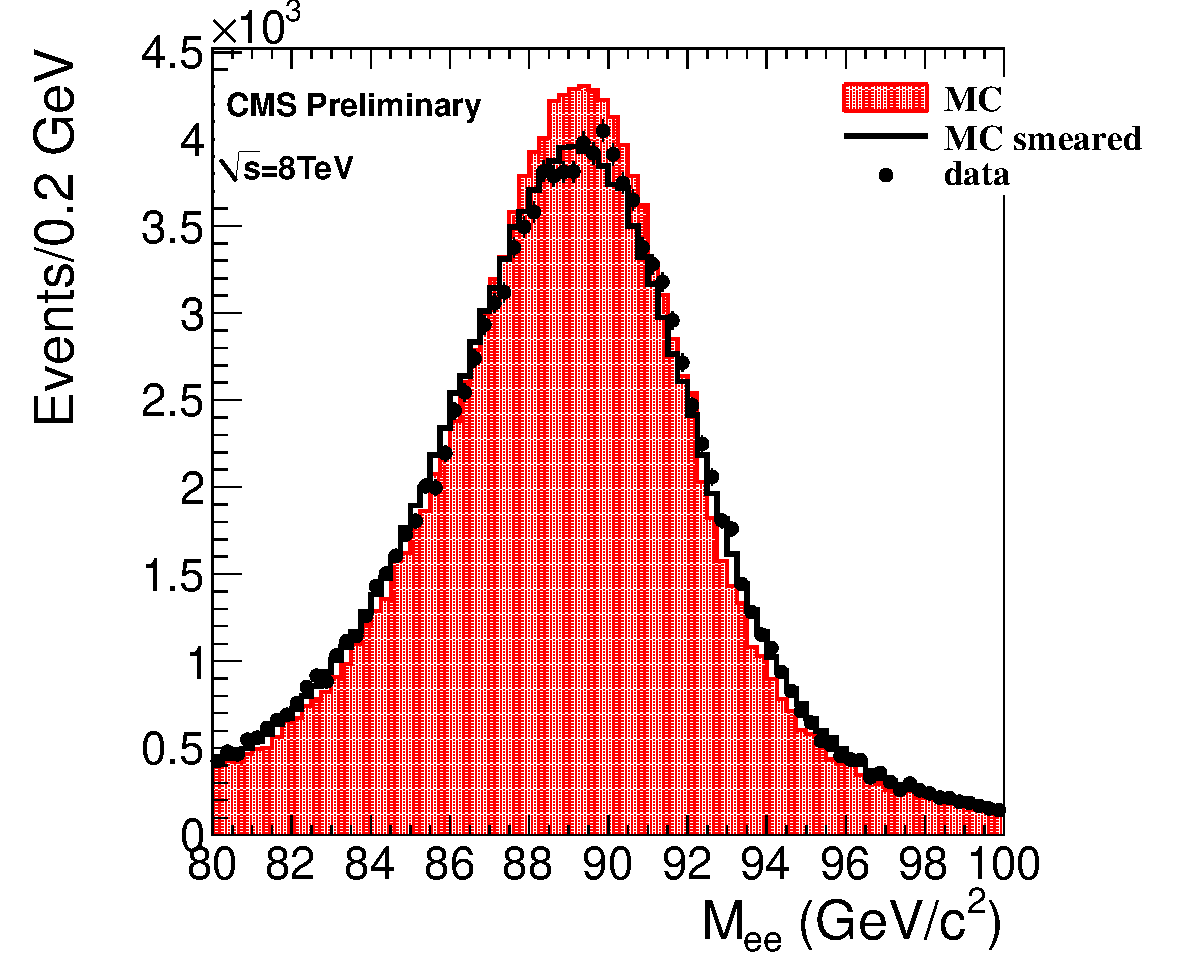
\includegraphics[width=0.48\textwidth]{ch3_comm_anal_comps/plots/smearing_EB_highEta_lowR9.pdf}
  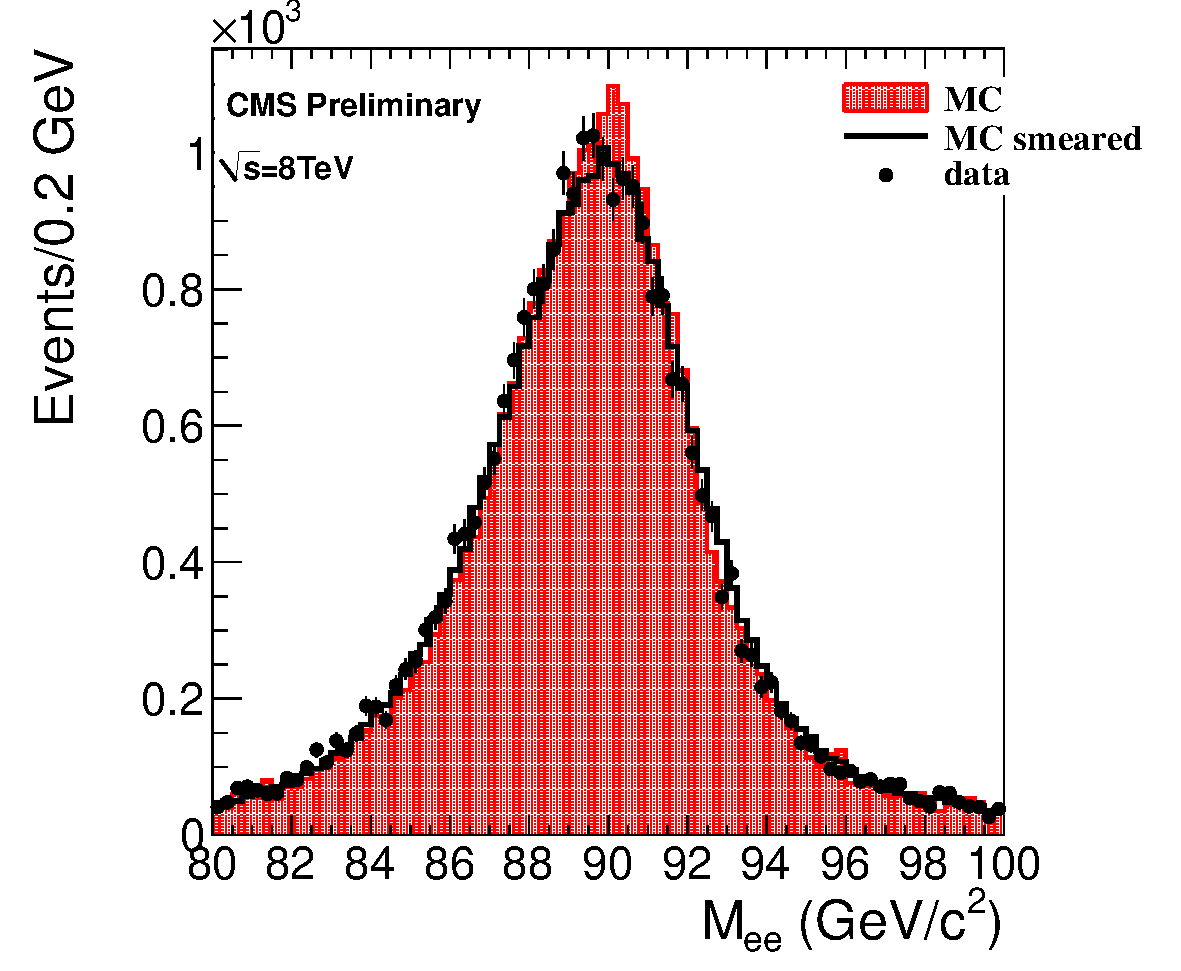
\includegraphics[width=0.48\textwidth]{ch3_comm_anal_comps/plots/smearing_EB_lowEta_highR9.pdf}
  \caption{The \Zee invariant mass shape comparison before and after the scale and smearing corrections are applied. Shown for 8~TeV for photons with $1.<|\eta|<1.444$ and $\rnine<0.94$ on the left and for photons with $|eta|<1.$ and $\rnine>0.4$ on the right.}
  \label{fig:scale_smearing_Zee}
\end{figure}

\begin{figure}
  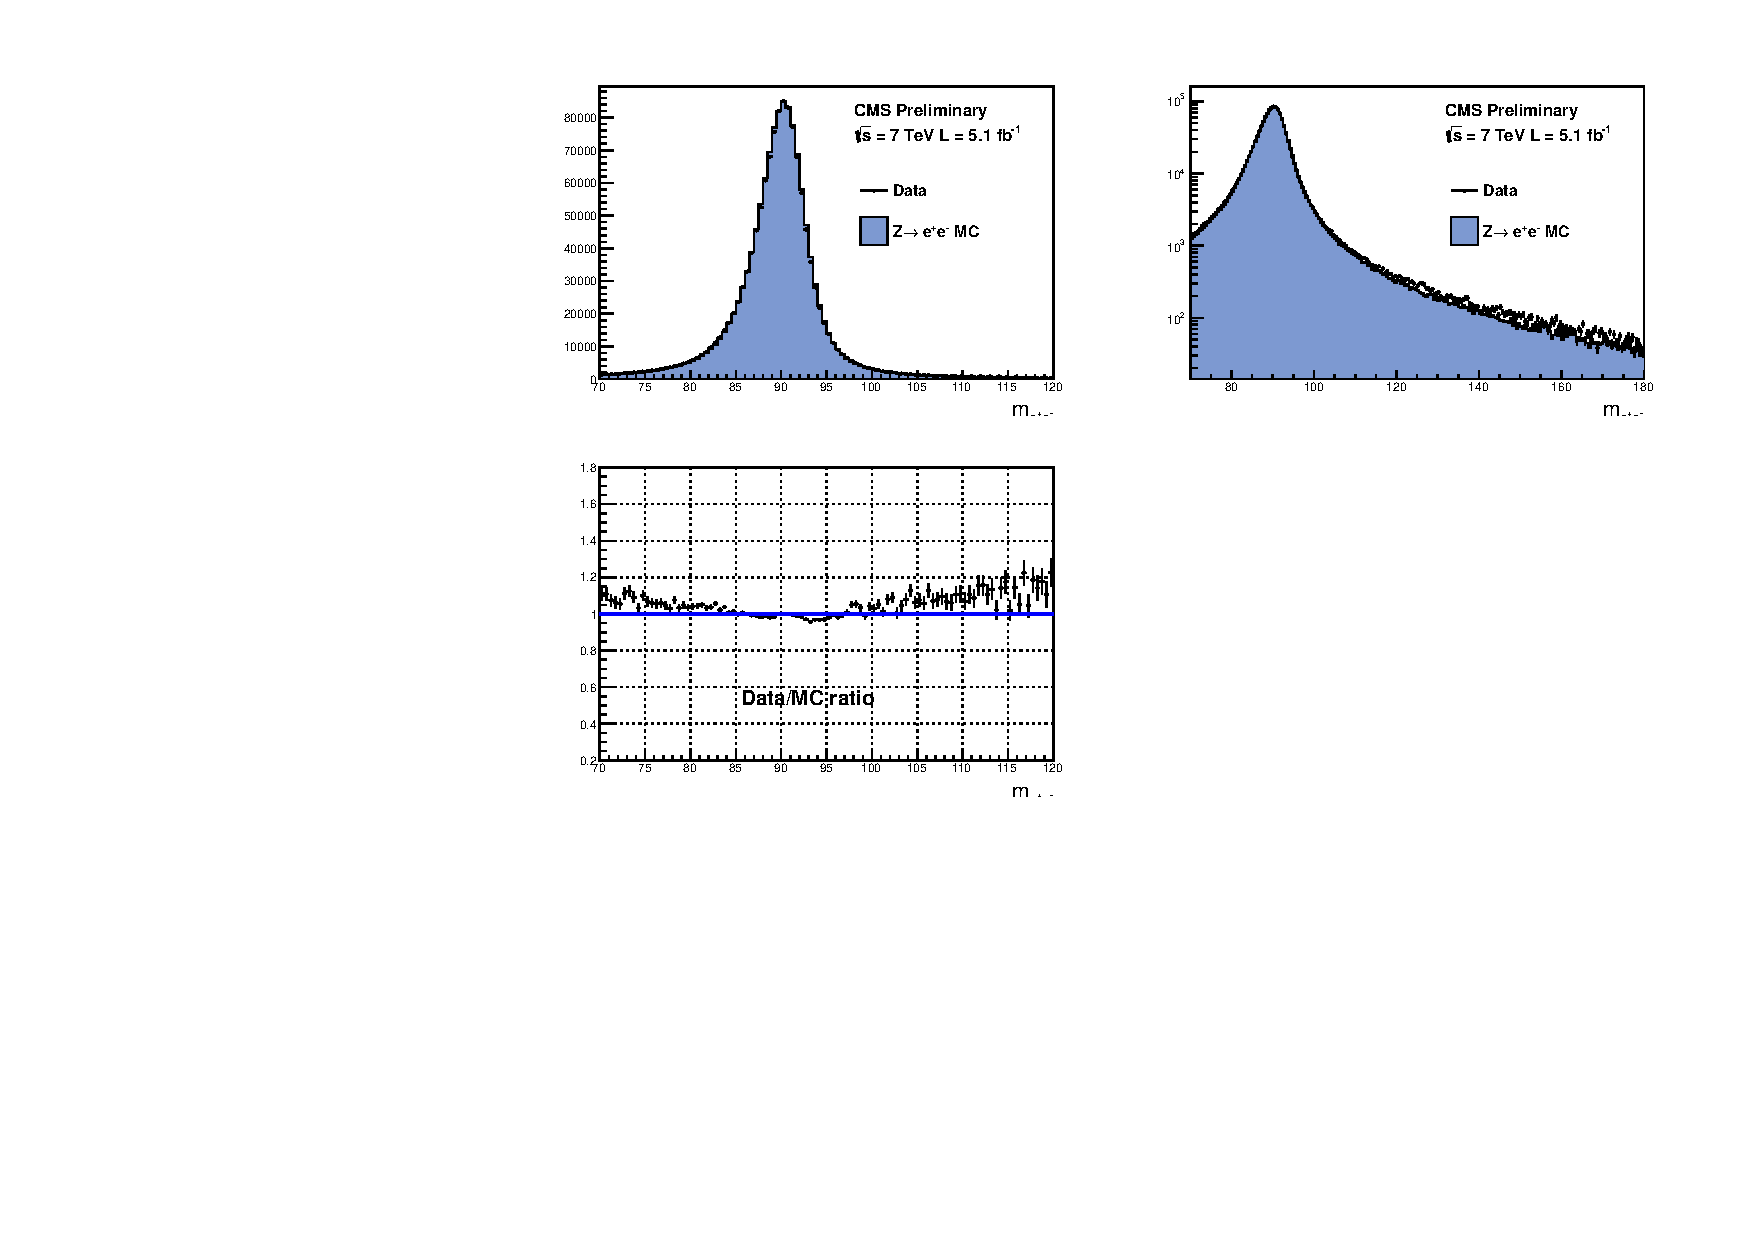
\includegraphics[width=0.9\textwidth]{ch3_comm_anal_comps/plots/smearing_mass_Zee_7TeV.pdf}
  \caption{The \Zee invariant mass distribution at 7TeV in data (black points) and \MC (blue histogram) for events which pass the analysis preselection in which the electron veto is inverted.}
  \label{fig:scale_smearing_analysis_7TeV}
\end{figure}

\begin{figure}
  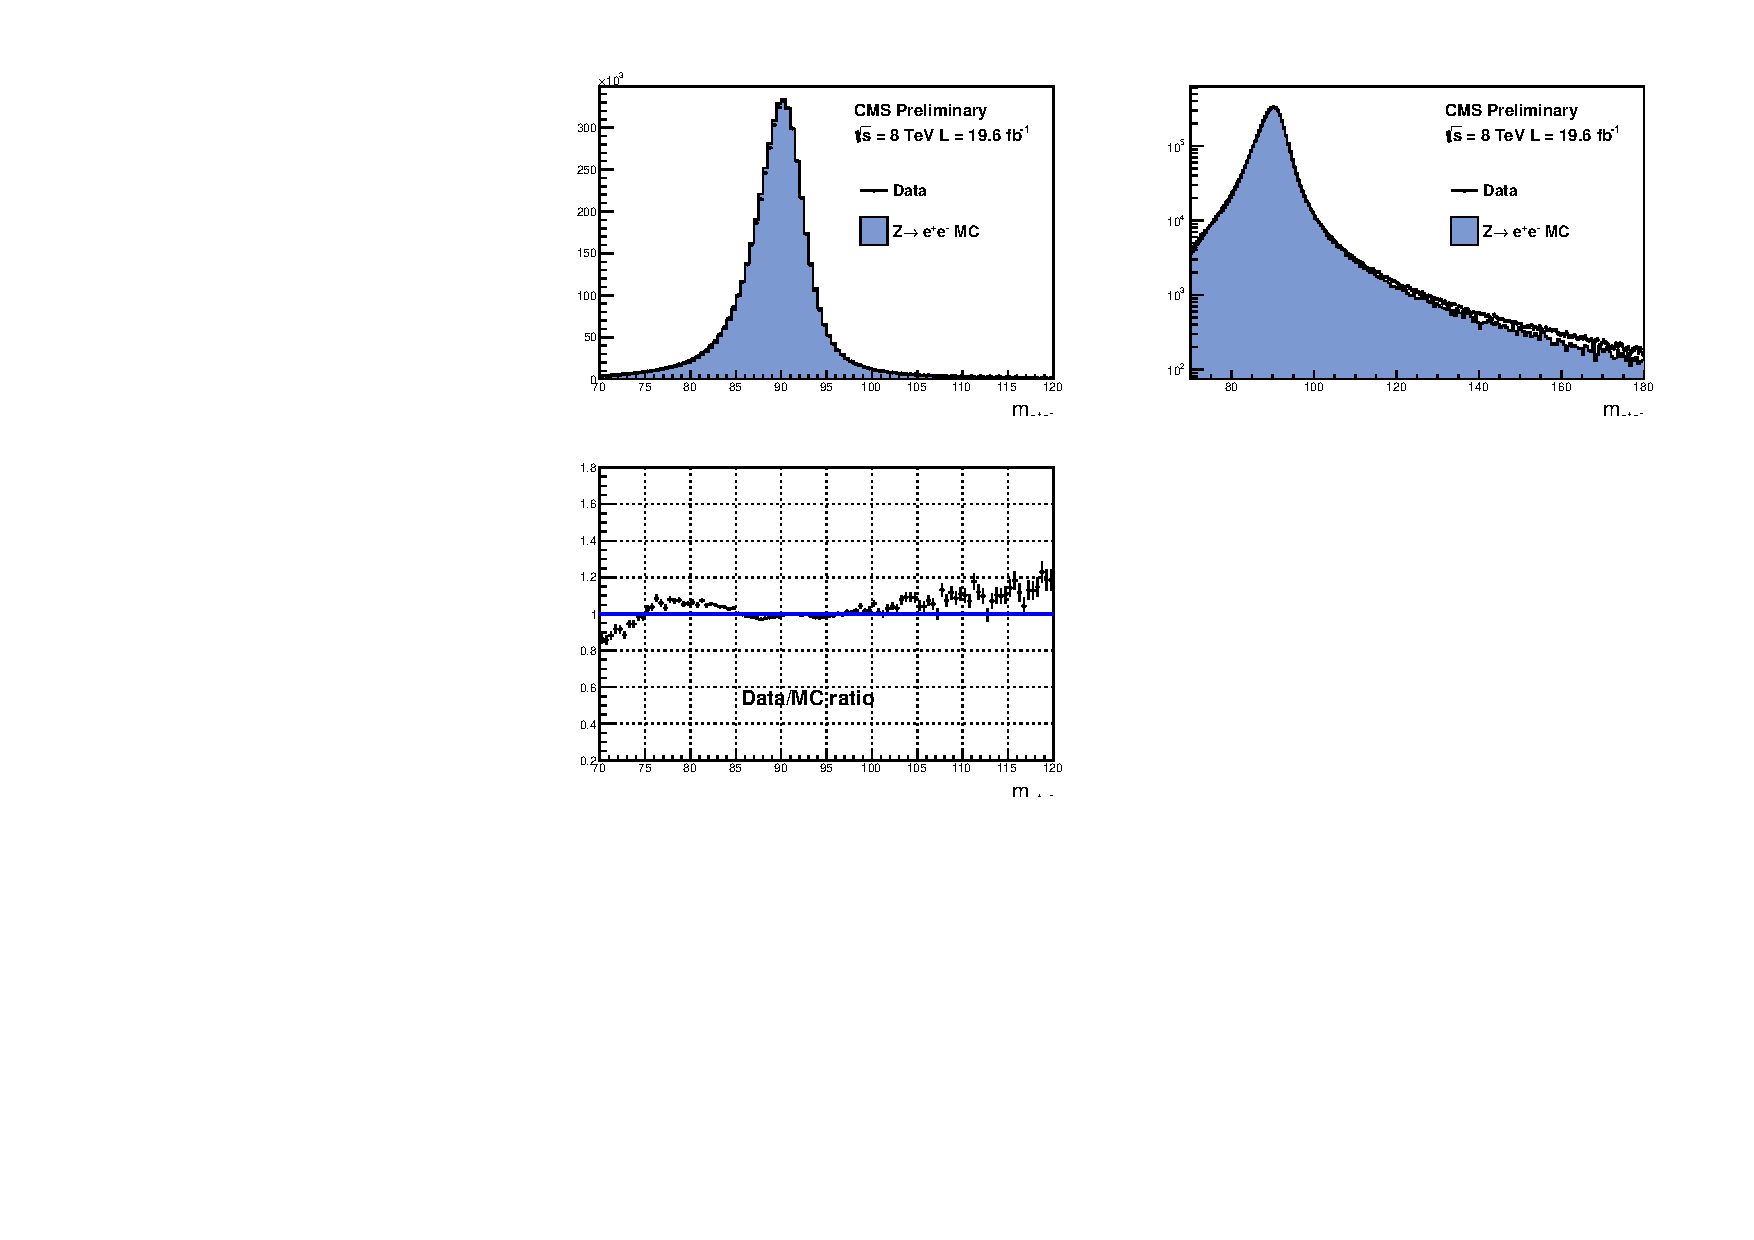
\includegraphics[width=0.9\textwidth]{ch3_comm_anal_comps/plots/smearing_mass_Zee_8TeV.pdf}
  \caption{The \Zee invariant mass distribution at 8TeV in data (black points) and \MC (blue histogram) for events which pass the analysis preselection in which the electron veto is inverted.}
  \label{fig:scale_smearing_analysis_8TeV}
\end{figure}

\section{Vertex reconstruction}
\label{sec:vtx_reco}

The resolution on the opening angle has a neglible effect if the correct vertex can be found within 10mm of the true interaction point. As seen in Sec.~\ref{sec:pileup_beamspot} the beamspot has an RMS spread of about 5~cm in the $z$ direction and there is an average of $\sim20$ vertices per bunch crossing. Because the beam direction is along the $z$-axis the spread of the vertex in the $x$ and $y$ directions is tiny (\red{number?}) and consequently mismeasurement of the primary vertex in the $x$-$y$ plane is small and has no impact on the mass resolution. By assigning the correct vertex to the diphoton pair, using other information in the tracking system, most of the mass resolution can be preserved. The method used to extract the primary vertex is a \BDT which exploits the correlation between the diphoton pair and the recoiling tracks from the underlying interaction as well as additional information in the tracking system from a photon conversion pair. The output of this per vertex \BDT is evaluated for each vertex in the event and the primary vertex is assigned as the one with the highest value of \BDT output (i.e.\ the value nearest 1.). In addition, it is possible to construct another \BDT whose output is proportional to the probability that the chosen vertex is the correct one (described in Sec.~\ref{sec:bdt_prob}). This probability becomes a useful discrimnanting variable for the analyses later on.

The vertex \BDT uses the following input variables:

\begin{itemize}
  \item $\sum\limits_{i} |\vec{p}{}^{\;i}_{T}|^{2}$ - the sum of the transverse momentum squared of all of the tracks which originate from this vertex, representing how hard the interaction is at this vertex.
  \item $\sum\limits_{i} \bigl(\vec{p}^{\;i}_{T} \cdot \frac{\vec{p}^{\gamma\gamma}_{T}}{|\vec{p}^{\gamma\gamma}_{T}|}\bigr)$ - the sum of the magnitude of the transverse momentum of each track orginating from this vertex relative to the transverse momentum of the diphoton system, representing the recoil of the tracks to the diphoton system.
  \item $\bigr(|\sum\limits_{i} \vec{p}^{\;i}_{T}| - \vec{p}^{\gamma\gamma}_{T}\bigl) / \bigr(|\sum\limits_{i} \vec{p}{}^{\;i}_{T}| + \vec{p}^{\gamma\gamma}_{T}\bigl)$ - the asymmetry between the diphoton system and the other tracks originating from this vertex.
  \item $|z_{v}-z_{c}|/\sigma_{c}$ - this is added for events which contain at least one photon conversion where $z_{v}$ is the $z$ position of the vertex in question and $z_{c}$ and $\sigma_{c}$ are the estimated $z$ position of the vertex from conversion information and its approximate error as defined below.
\end{itemize}

For events which contain at least one photon conversion, the conversion tracks and/or the conversion momentum can be used to point back to the beam line and estimate the vertex position. This can be acheived in one of two ways. In cases where the conversion occurs early, i.e.\ in one of the first layers of the tracking system, then the two electron legs of the conversion will leave two clean and distinct tracks. This means that the momentum of the conversion pair can be accurately reconstructed and used to point from the conversion vertex position back to the beam line and thus the nearest primary vertex. In cases where the conversion occurs late in the tracking system there are not enough track hits to accurately reconstruct the momentum of the conversion pair, however the incident position of the photon at the \ECAL face is well known in this case, so the line which connects the \ECAL position with the conversion vertex can be used to point back to the beam line. This is diagramtically represented in Figure~\ref{fig:conv_diags} for both cases.

\begin{figure}
  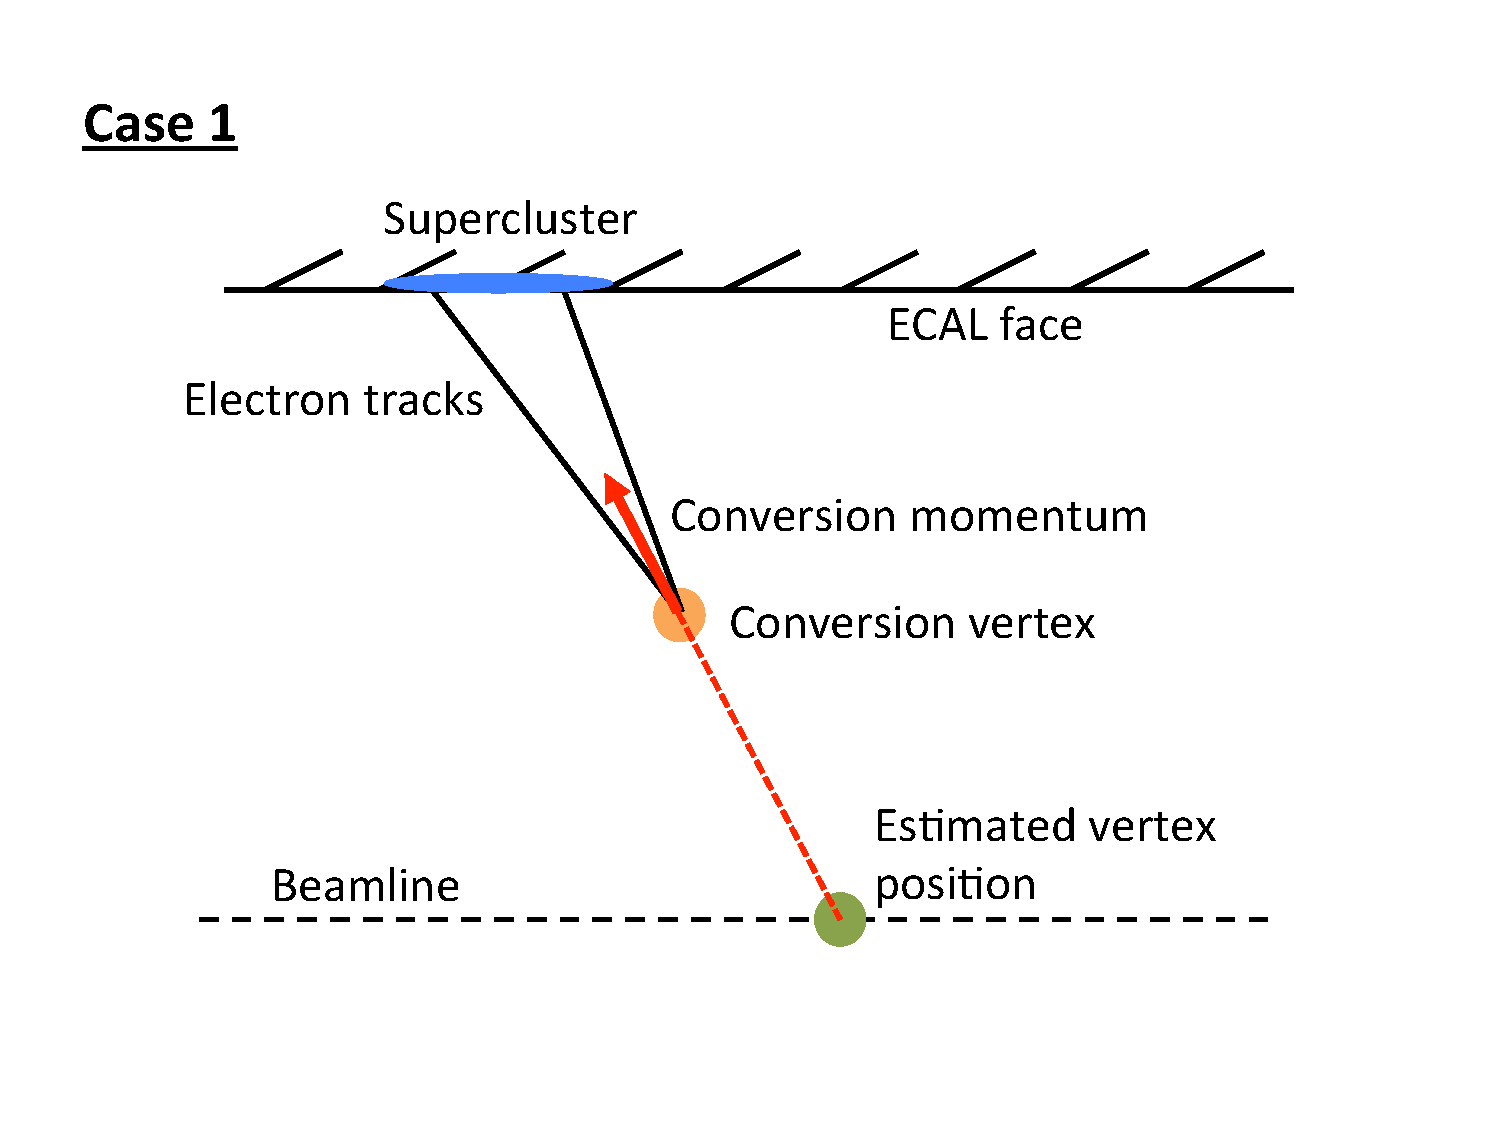
\includegraphics[width=0.49\textwidth]{ch3_comm_anal_comps/plots/ConversionDiagCase1.pdf}
  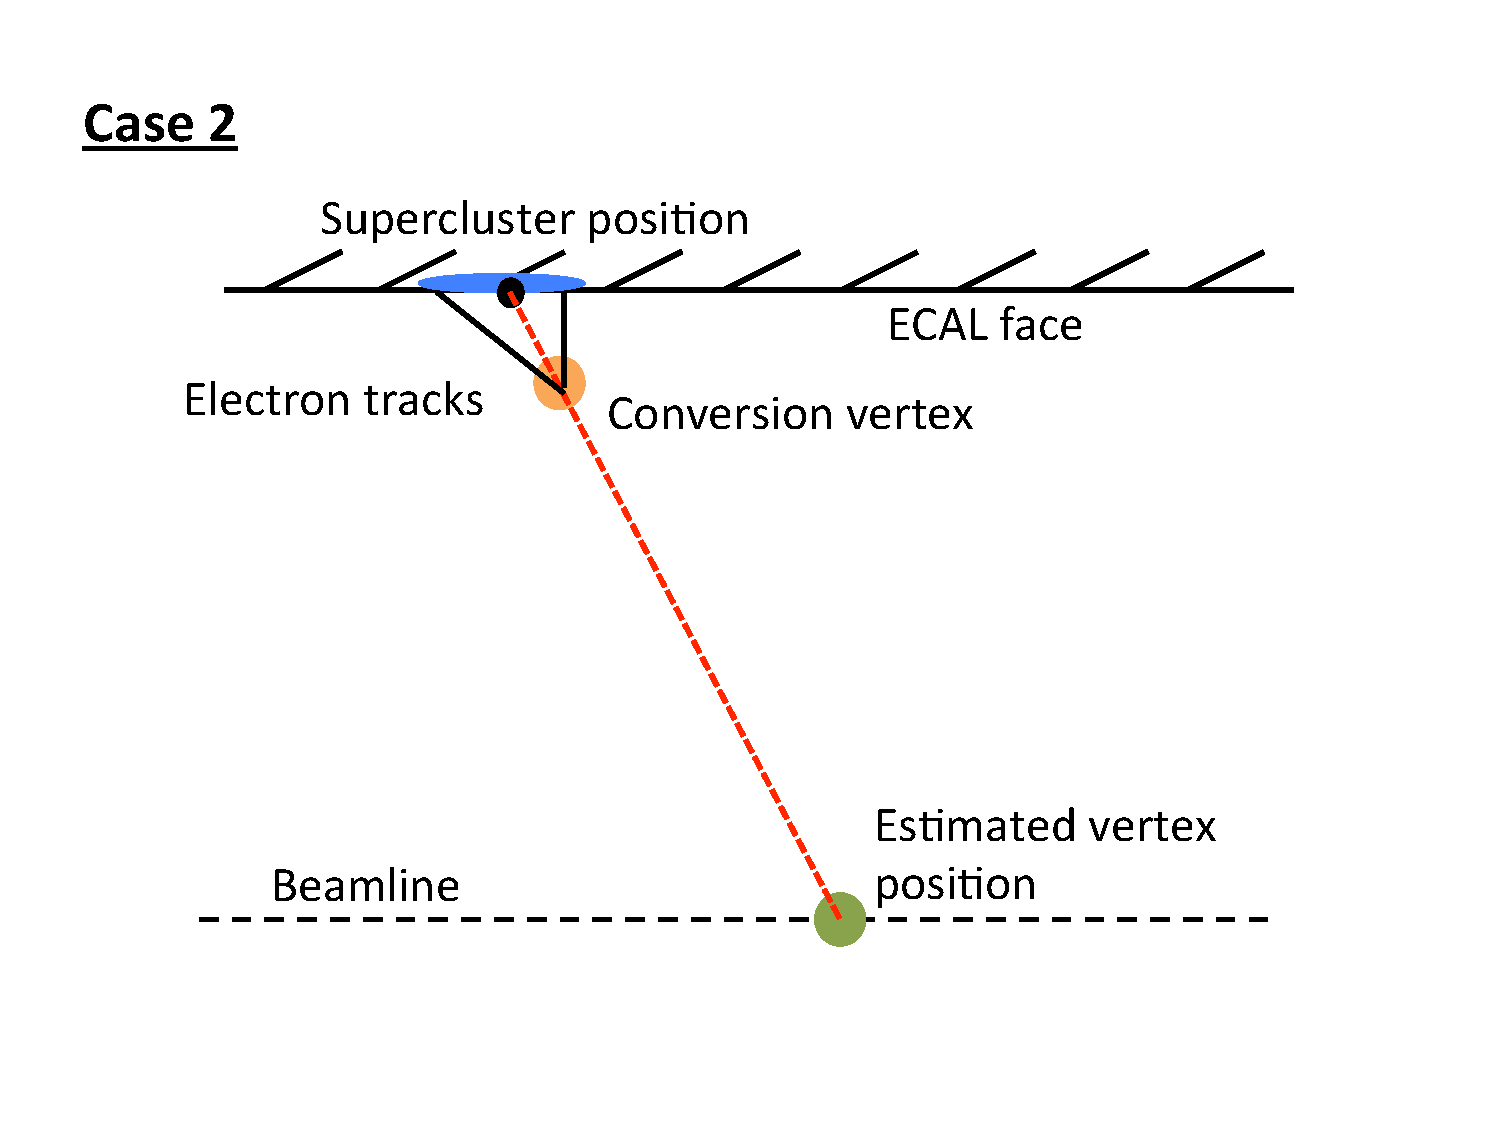
\includegraphics[width=0.49\textwidth]{ch3_comm_anal_comps/plots/ConversionDiagCase2.pdf}
  \caption{A representation of the two methods for locating the primary vertex using photon conversion information. The left plot is for cases where the conversion occurs early enough in the tracker that the two electron tracks can be used to construct the converted pair momentum which is combined with the conversion vertex position to point back to the beam line. The right plot is for cases where the conversion occurs late in the tracker and the energy weighted supercluster position and the conversion vertex position are used to point back to the beam line.}
  \label{fig:conv_diags}
\end{figure}

For Case 1 conversions the primary vertex $z$ position is calculated as,

\begin{equation}
  z_{c} = z_{conv} - r_{conv}\cot(\alpha),
\end{equation}
where $z_{conv}$ is the z position of the conversion vertex, $r_{conv}$ is the distance of the conversion vertex from the beam line and $\alpha$ is the angle between the beam line and the conversion momentum.

For Case 2 conversions the primary vertex $z$ position is calculated as,

\begin{equation}
  z_{c} = \frac{z_{conv}-r_{conv}}{(r_{SC}-r_{conv})(z_{SC}-z_{conv})},
\end{equation}
where $z_{conv}$ and $z_{SC}$ are the $z$ positions of the conversion vertex and supercluster respectively, and $r_{conv}$ and $r_{SC}$ are the distance of the conversion vertex and the supercluster from the beamline.

There are 6 regions of the tracking system (refer back to Figure~\ref{fig:cms_tracker}). When the conversion vertex is located in one of the inner regions; Pixel Barrel, Pixel Forward, TID, the Case 1 
conversion information is included in the \BDT, otherwise the Case 2 conversion information is used. The resolution on the primary vertex position in conversions is estimated per tracking region by calulating the effective width \footnote{Half the narrowest interval which contains 68.3\% of the distribution} of the distribution of the difference between the $z$ position of the primary vertex without conversion information and the $z$ position of the primary vertex using conversion information alone, $\Delta z=z_{v}-z_{c}$. Consequently the fourth input variable to the \BDT, shown in the list above as $|z_{v}-z_{c}|/\sigma_{c}$, is effectively a pull distribution for the conversion vertex. The \BDT will favour vertices whose value of this variable is near zero.

The \BDT is trained on a sample of \Hgg \MC events. It is tested with a statistically independent sample and further validated using \Zmumu decays in data and \MC. The efficiency is measured in data using the \Zmumu channel where the muon tracks are removed from the \BDT variables to simulate a diphoton like situation in data. The distributions of the input variables are shown for the \Hgg training sample in Figure~\ref{fig:vertex_bdt_inputs} (\red{probably unnecessary}). The \BDT response is shown for \Zmumu data and \MC for both the signal (right vertex) and background (wrong vertex) in Figure~\ref{fig:vertex_bdt_response}. The chosen primary vertex is the one which gives the highest score \BDT output. The efficiency of the vertex selection as a function of the $Z$ \pT and the number of reconstructed vertices as measured in \Zmumu data and \MC samples is shown in Figure~\ref{fig:vertex_bdt_efficiency}. 

\begin{figure}
  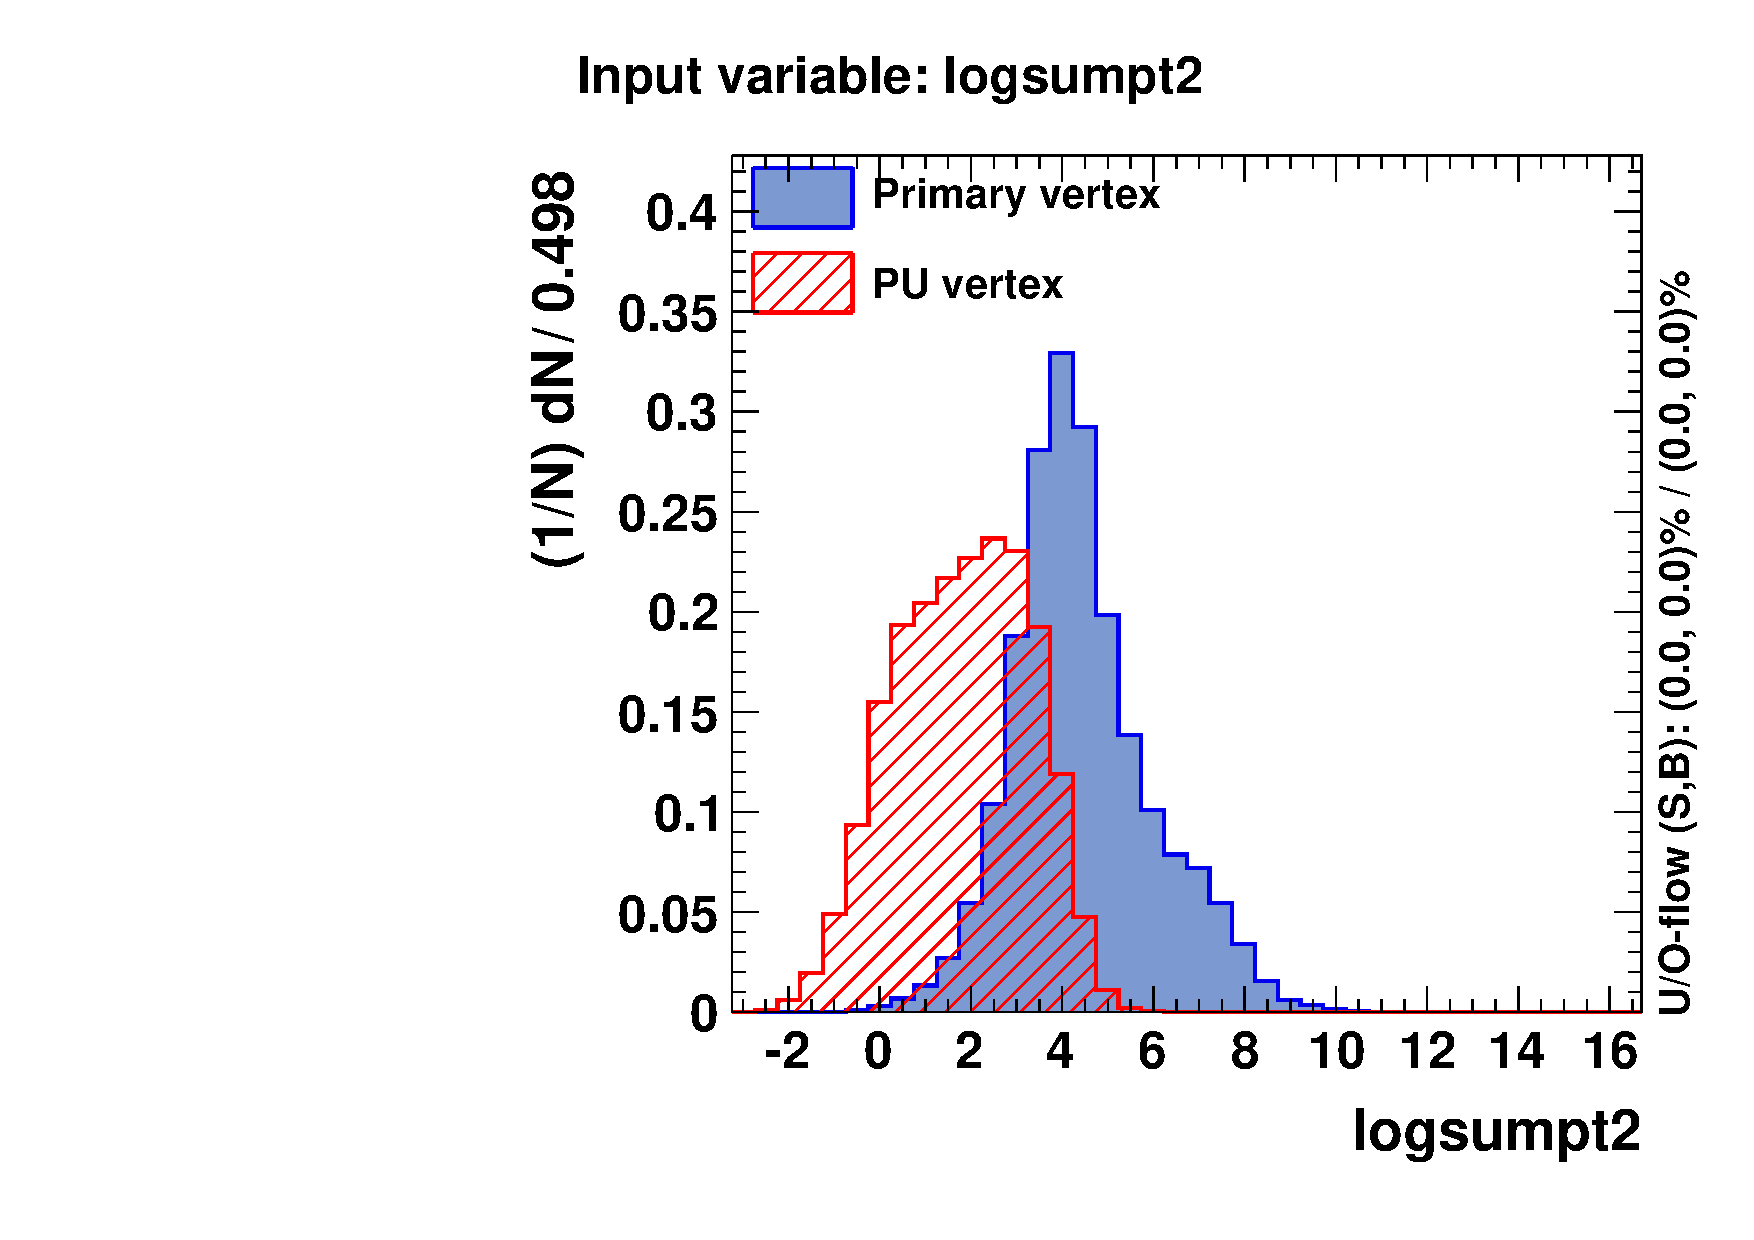
\includegraphics[width=0.48\textwidth]{ch3_comm_anal_comps/plots/vertex_bdt_input0.pdf}
  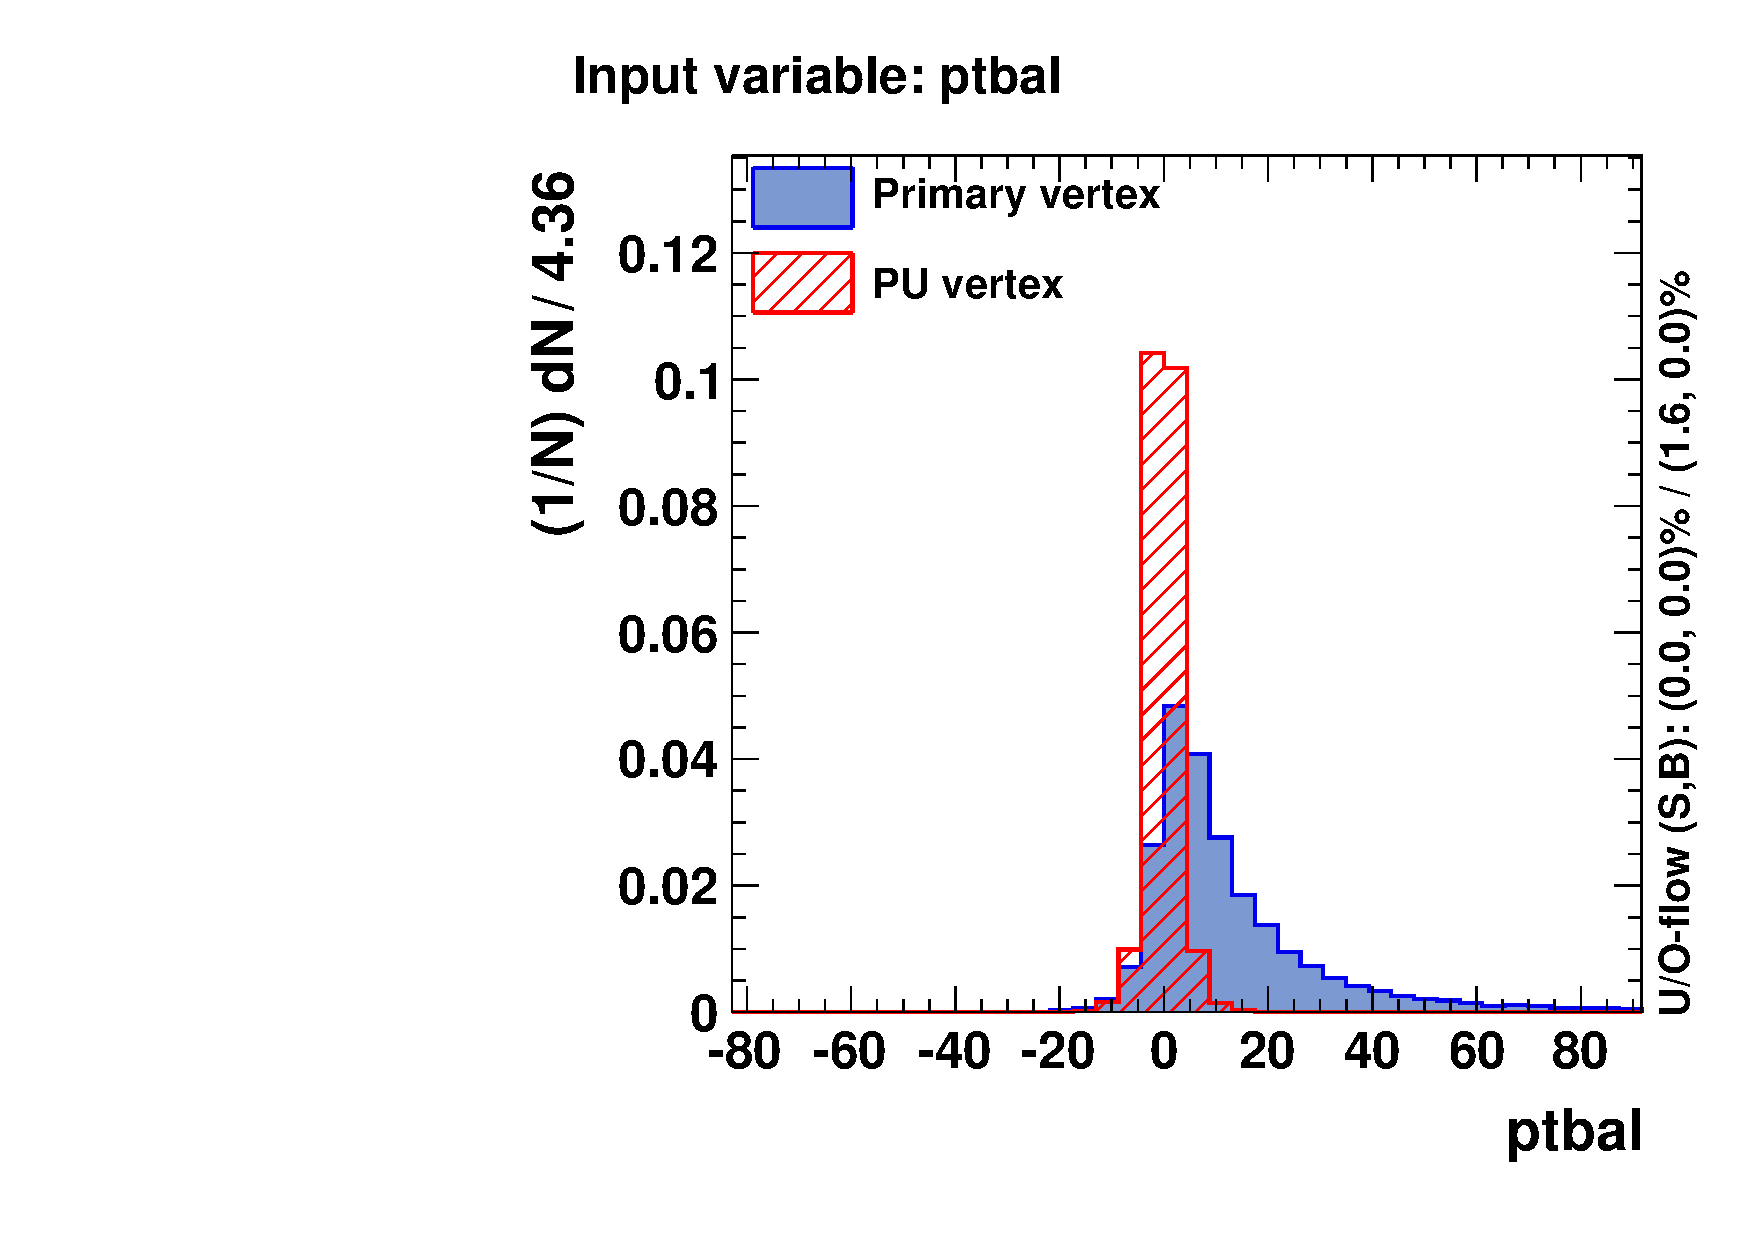
\includegraphics[width=0.48\textwidth]{ch3_comm_anal_comps/plots/vertex_bdt_input1.pdf} \\
  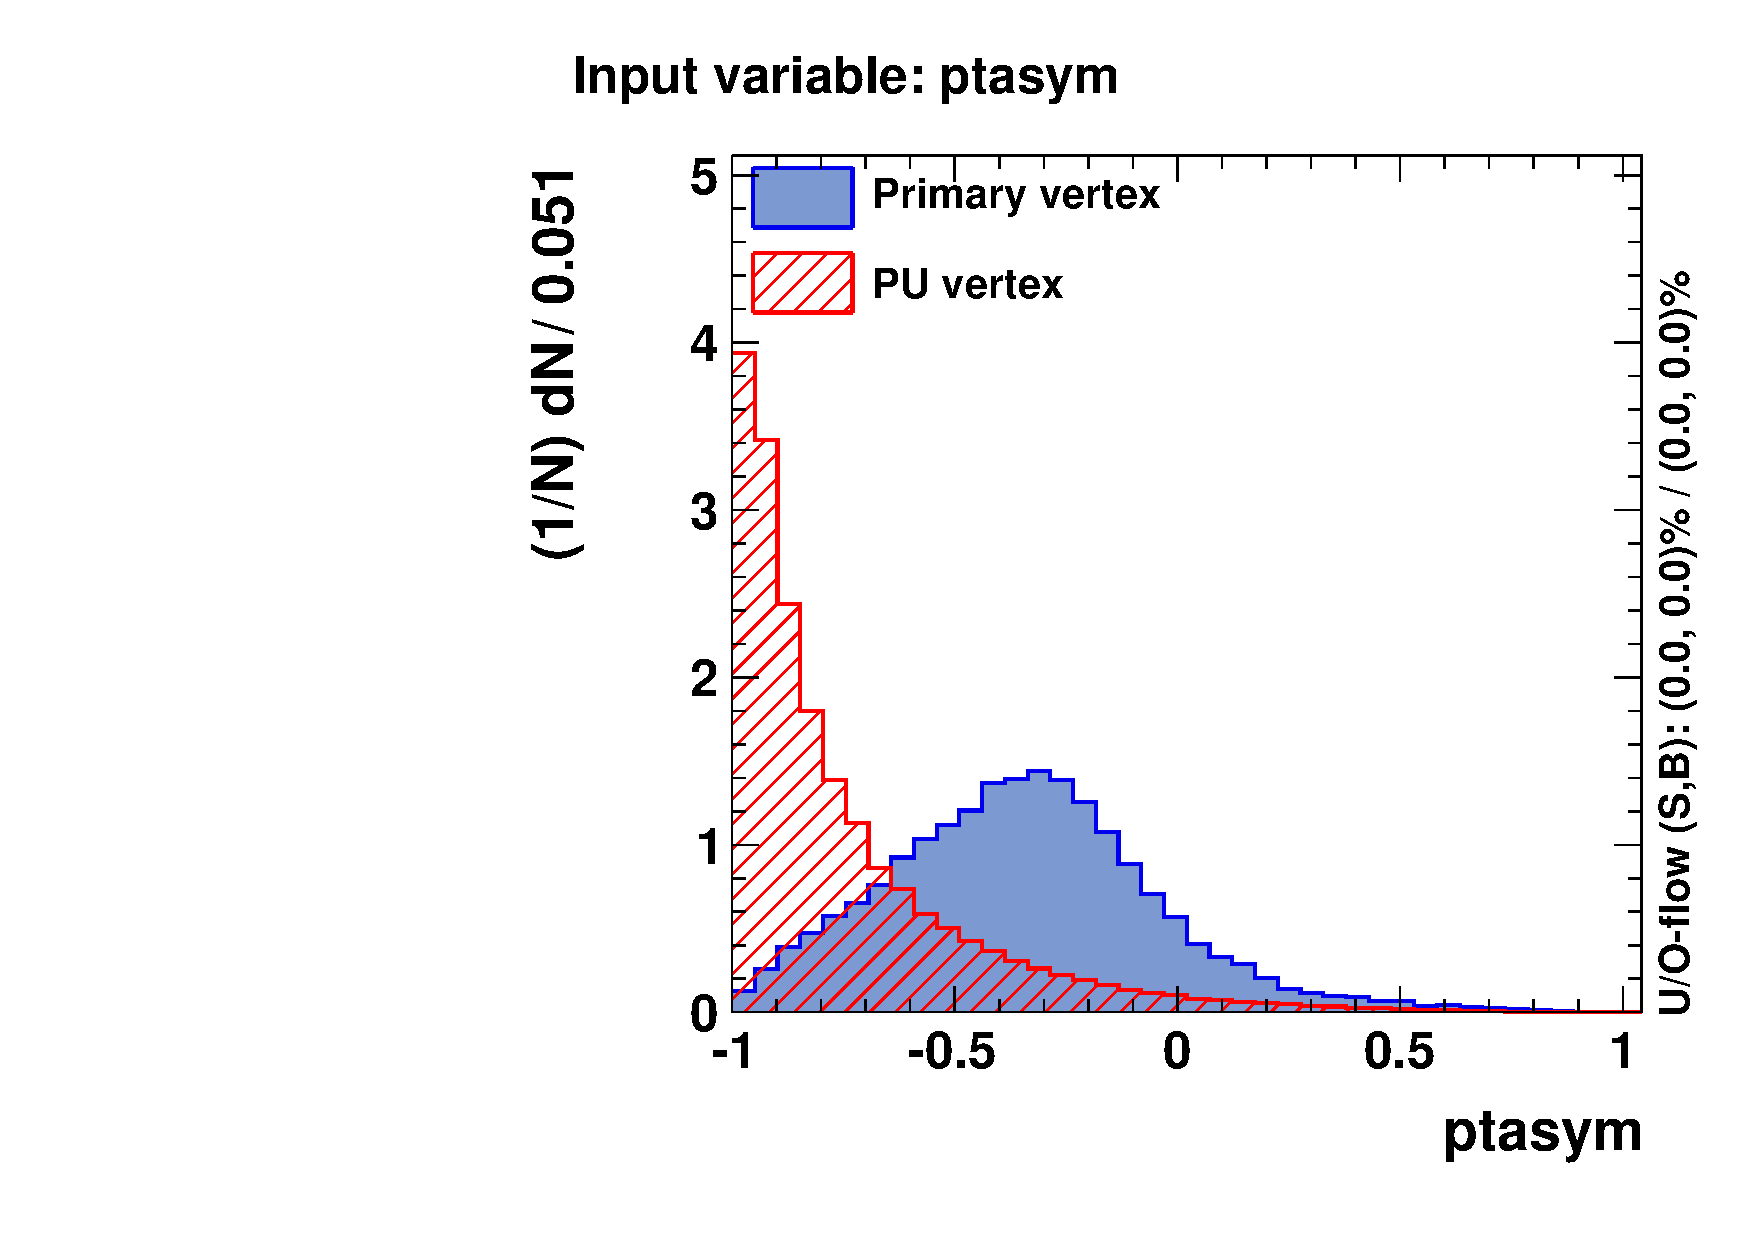
\includegraphics[width=0.48\textwidth]{ch3_comm_anal_comps/plots/vertex_bdt_input2.pdf}
  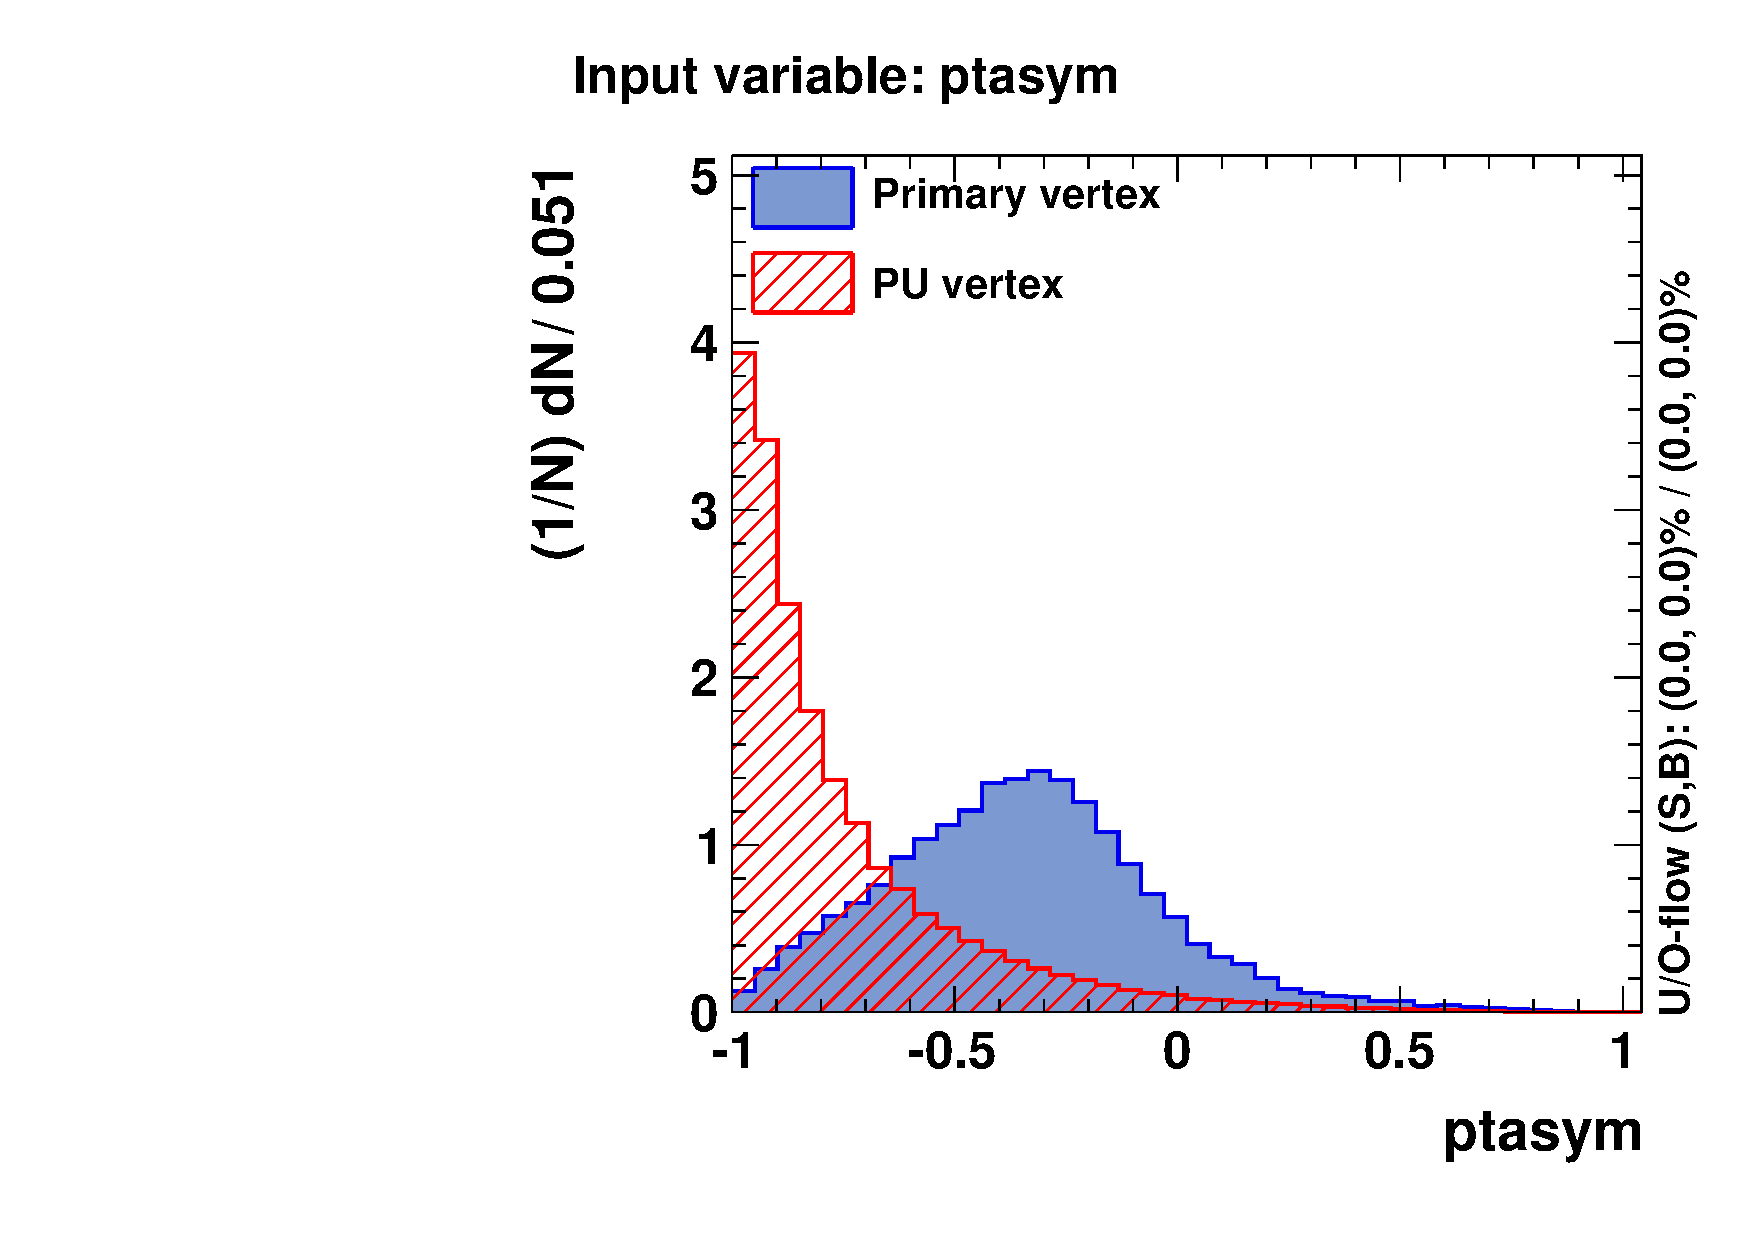
\includegraphics[width=0.48\textwidth]{ch3_comm_anal_comps/plots/vertex_bdt_input3.pdf}
  \caption{Distributions of the input variables for the vertex \BDT in the \MC \Hgg training (points) and test (filled) samples at 8TeV. Shown for the target primary vertex (blue histograms) and the background pileup vertices (red histograms). \red{Plots need updating, tidying and labelling correctly.}}
  \label{fig:vertex_bdt_inputs}
\end{figure}

\begin{figure}
  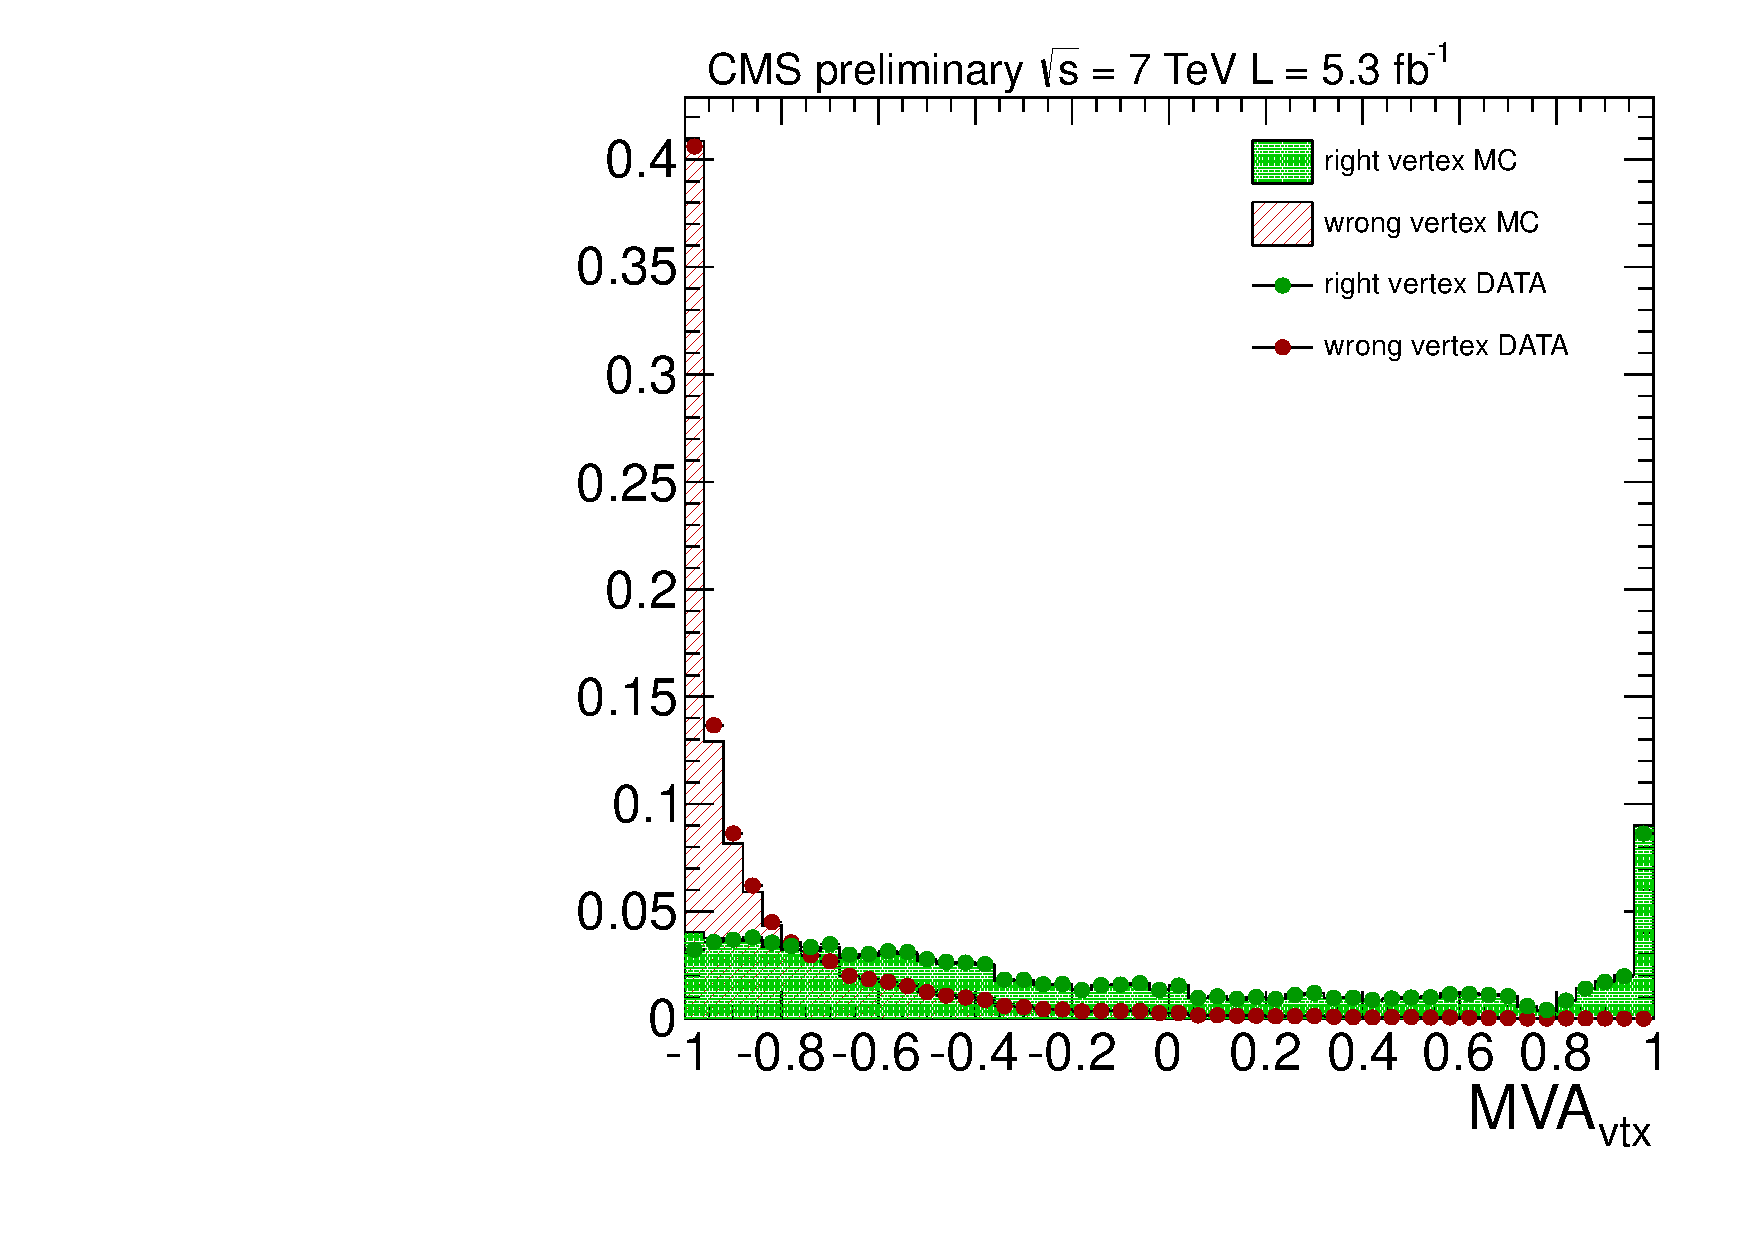
\includegraphics[width=0.48\textwidth]{ch3_comm_anal_comps/plots/vertex_bdt_output_7TeV.pdf}
  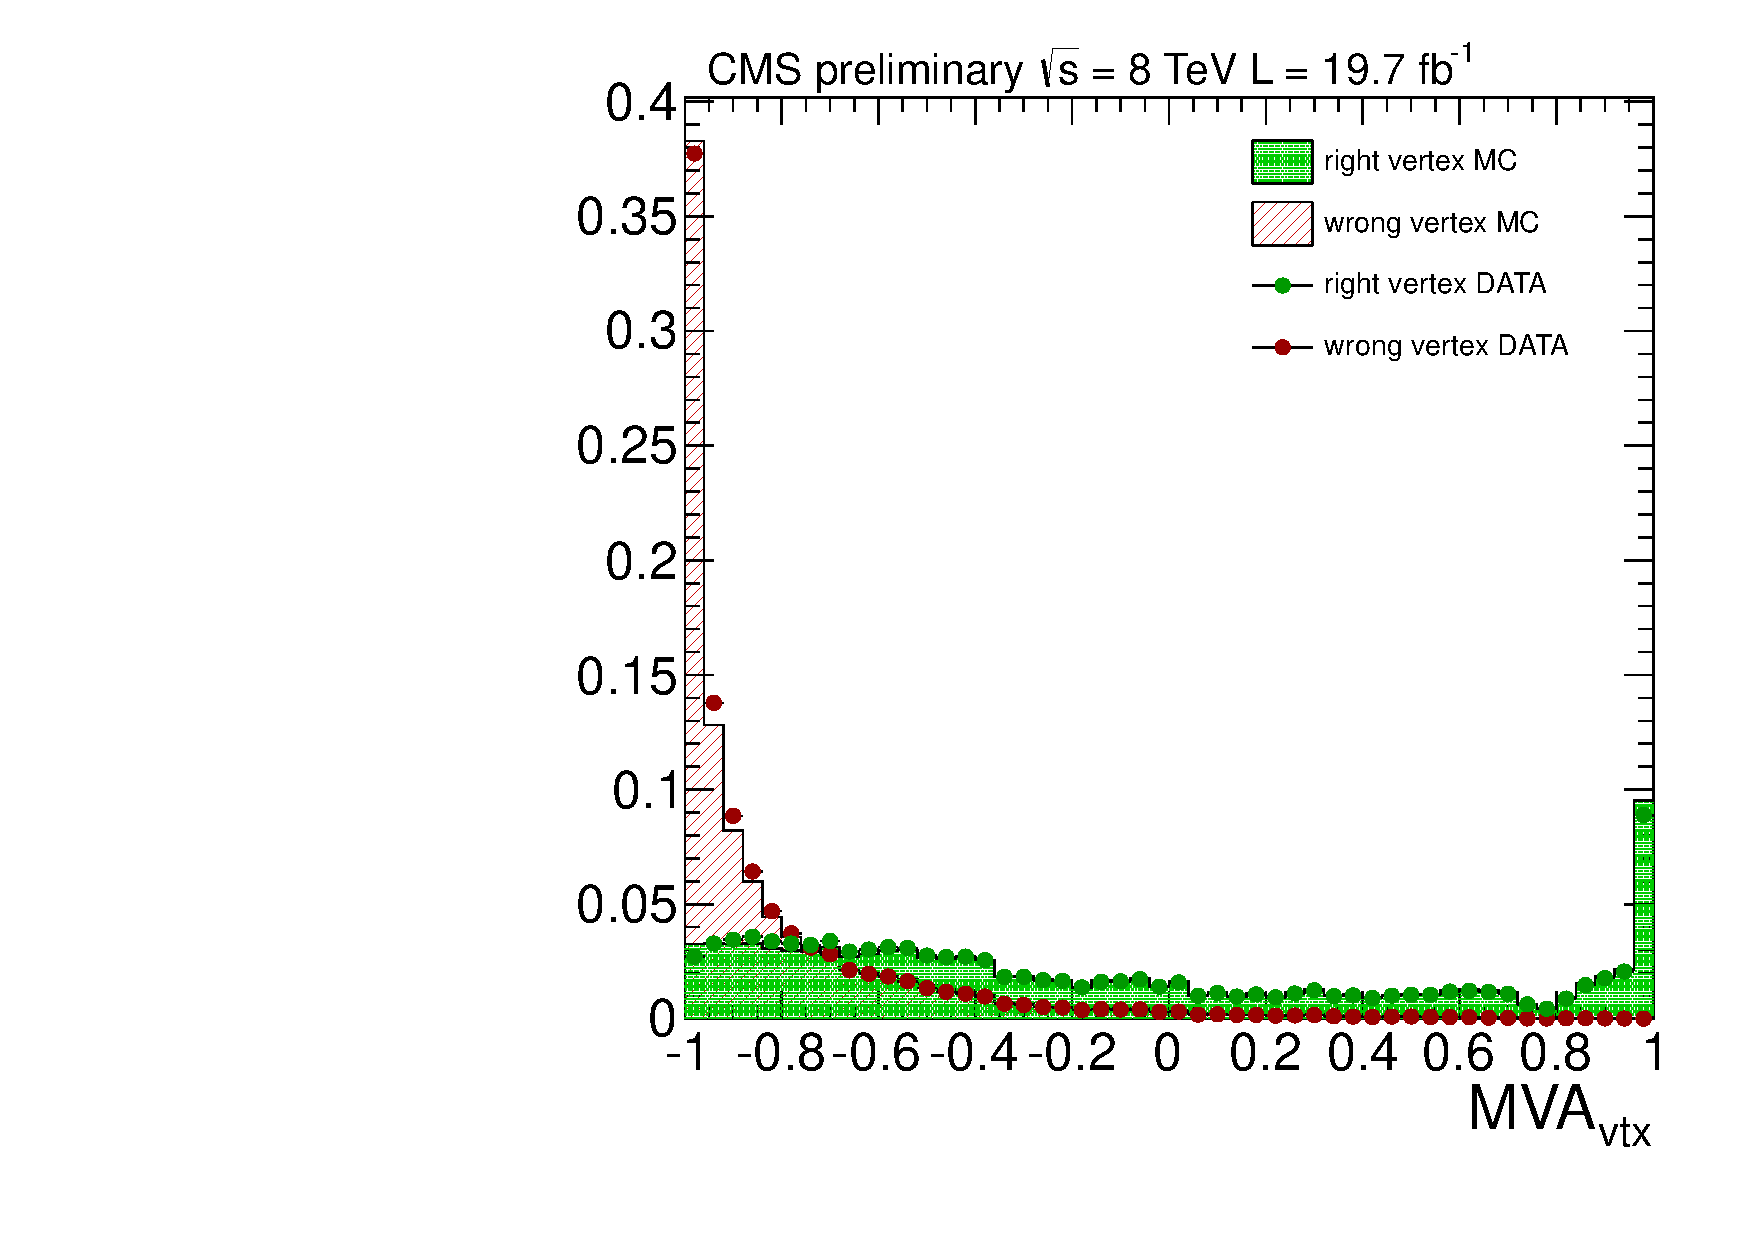
\includegraphics[width=0.48\textwidth]{ch3_comm_anal_comps/plots/vertex_bdt_output_8TeV.pdf}
  \caption{The vertex \BDT response for \Zmumu events in data (points) and MC (filled) for the primary vertex (green) and the background pileup vertices (red).}
  \label{fig:vertex_bdt_response}
\end{figure}

\begin{figure}
  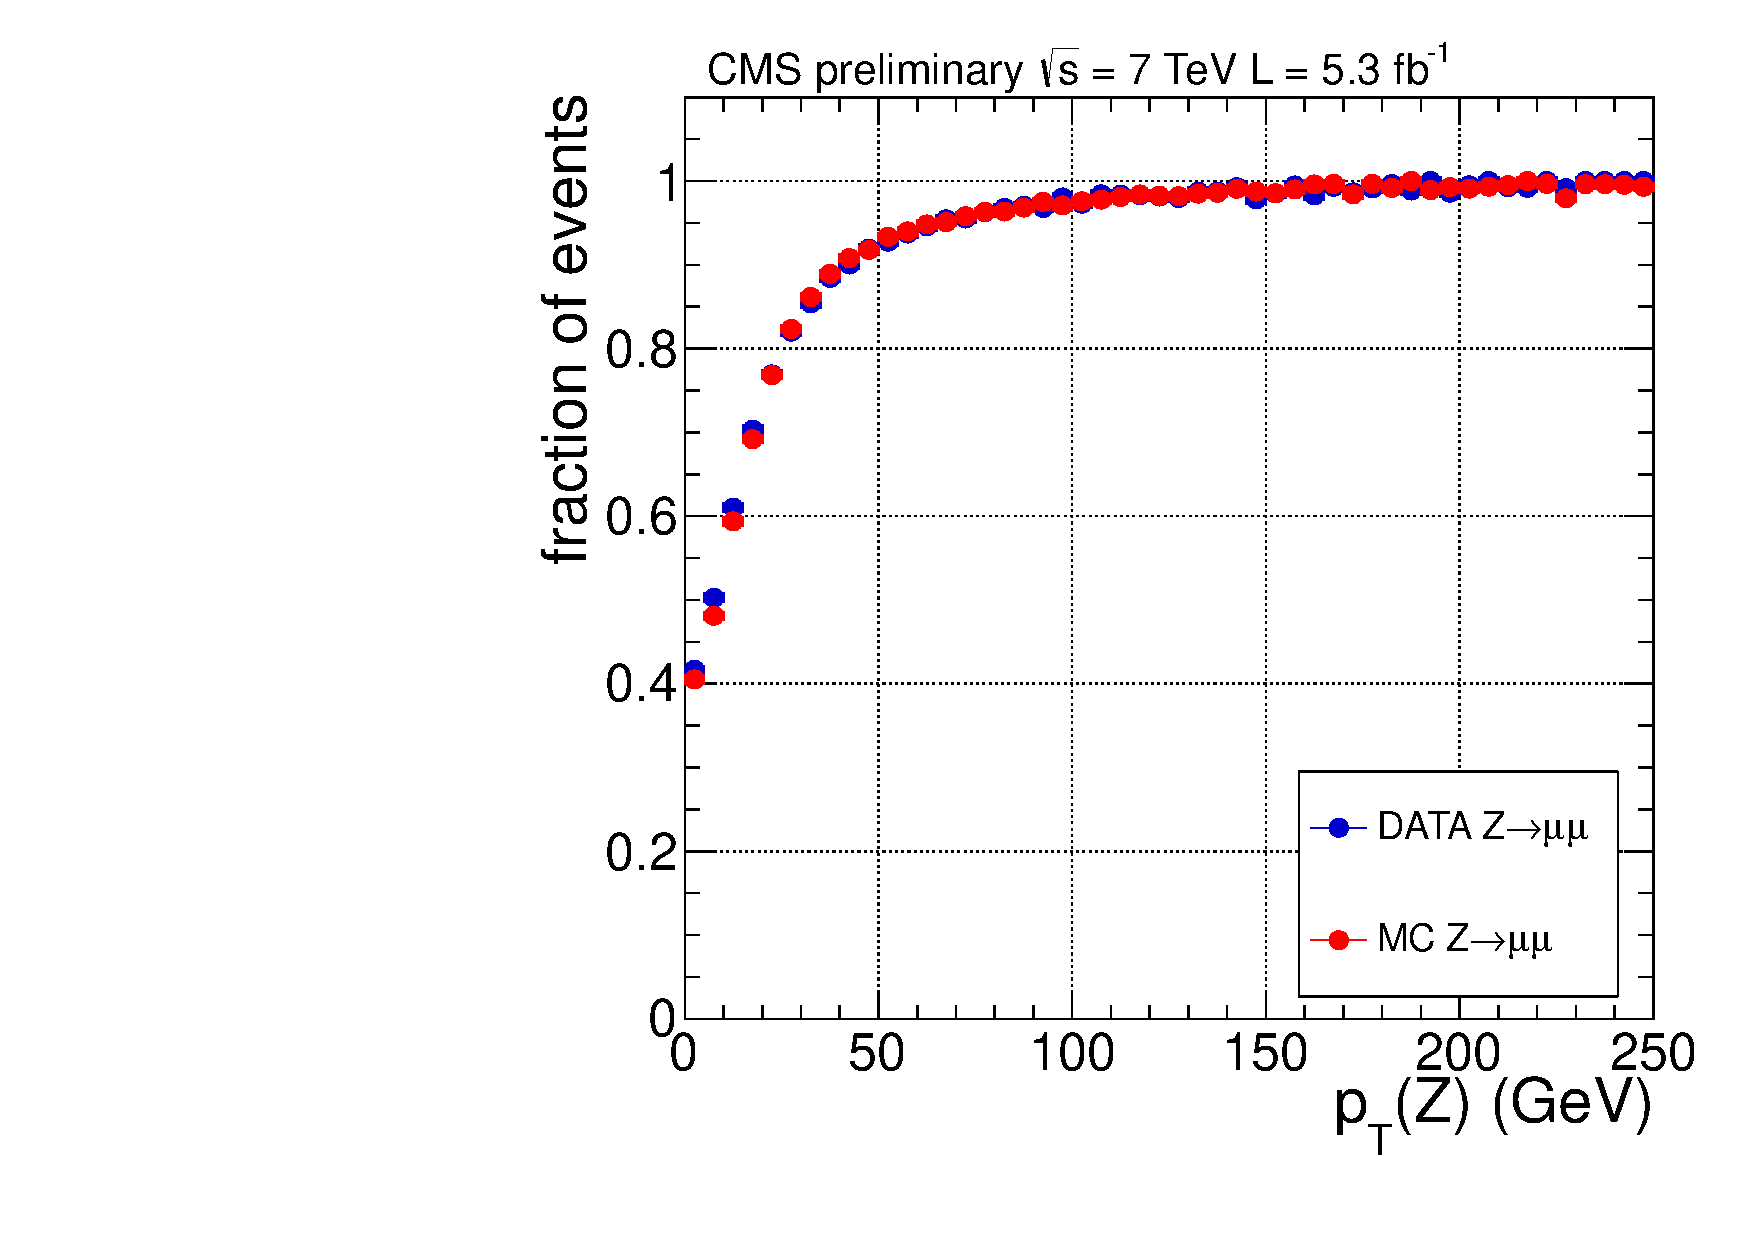
\includegraphics[width=0.48\textwidth]{ch3_comm_anal_comps/plots/vertex_bdt_efficiency_pt_7TeV.pdf}
  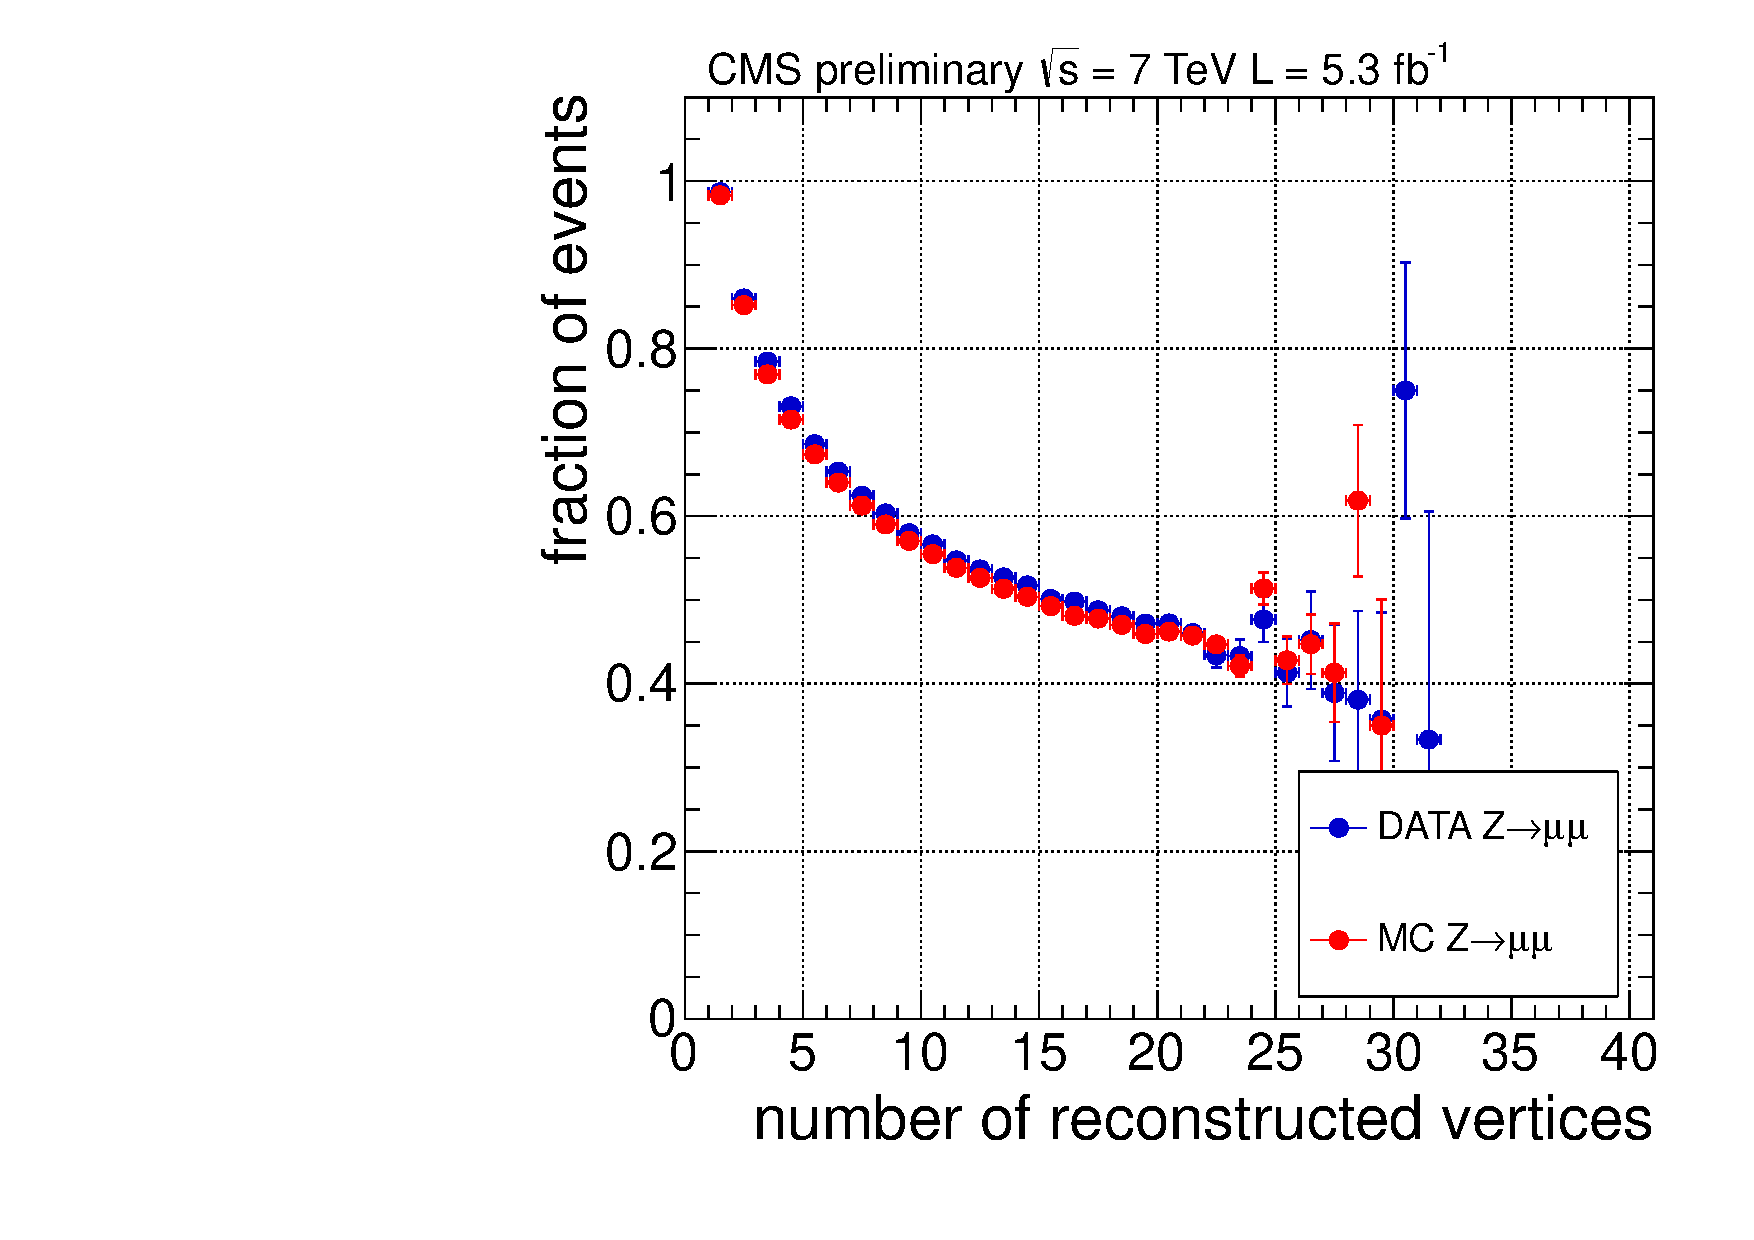
\includegraphics[width=0.48\textwidth]{ch3_comm_anal_comps/plots/vertex_bdt_efficiency_nvtx_7TeV.pdf} \\
  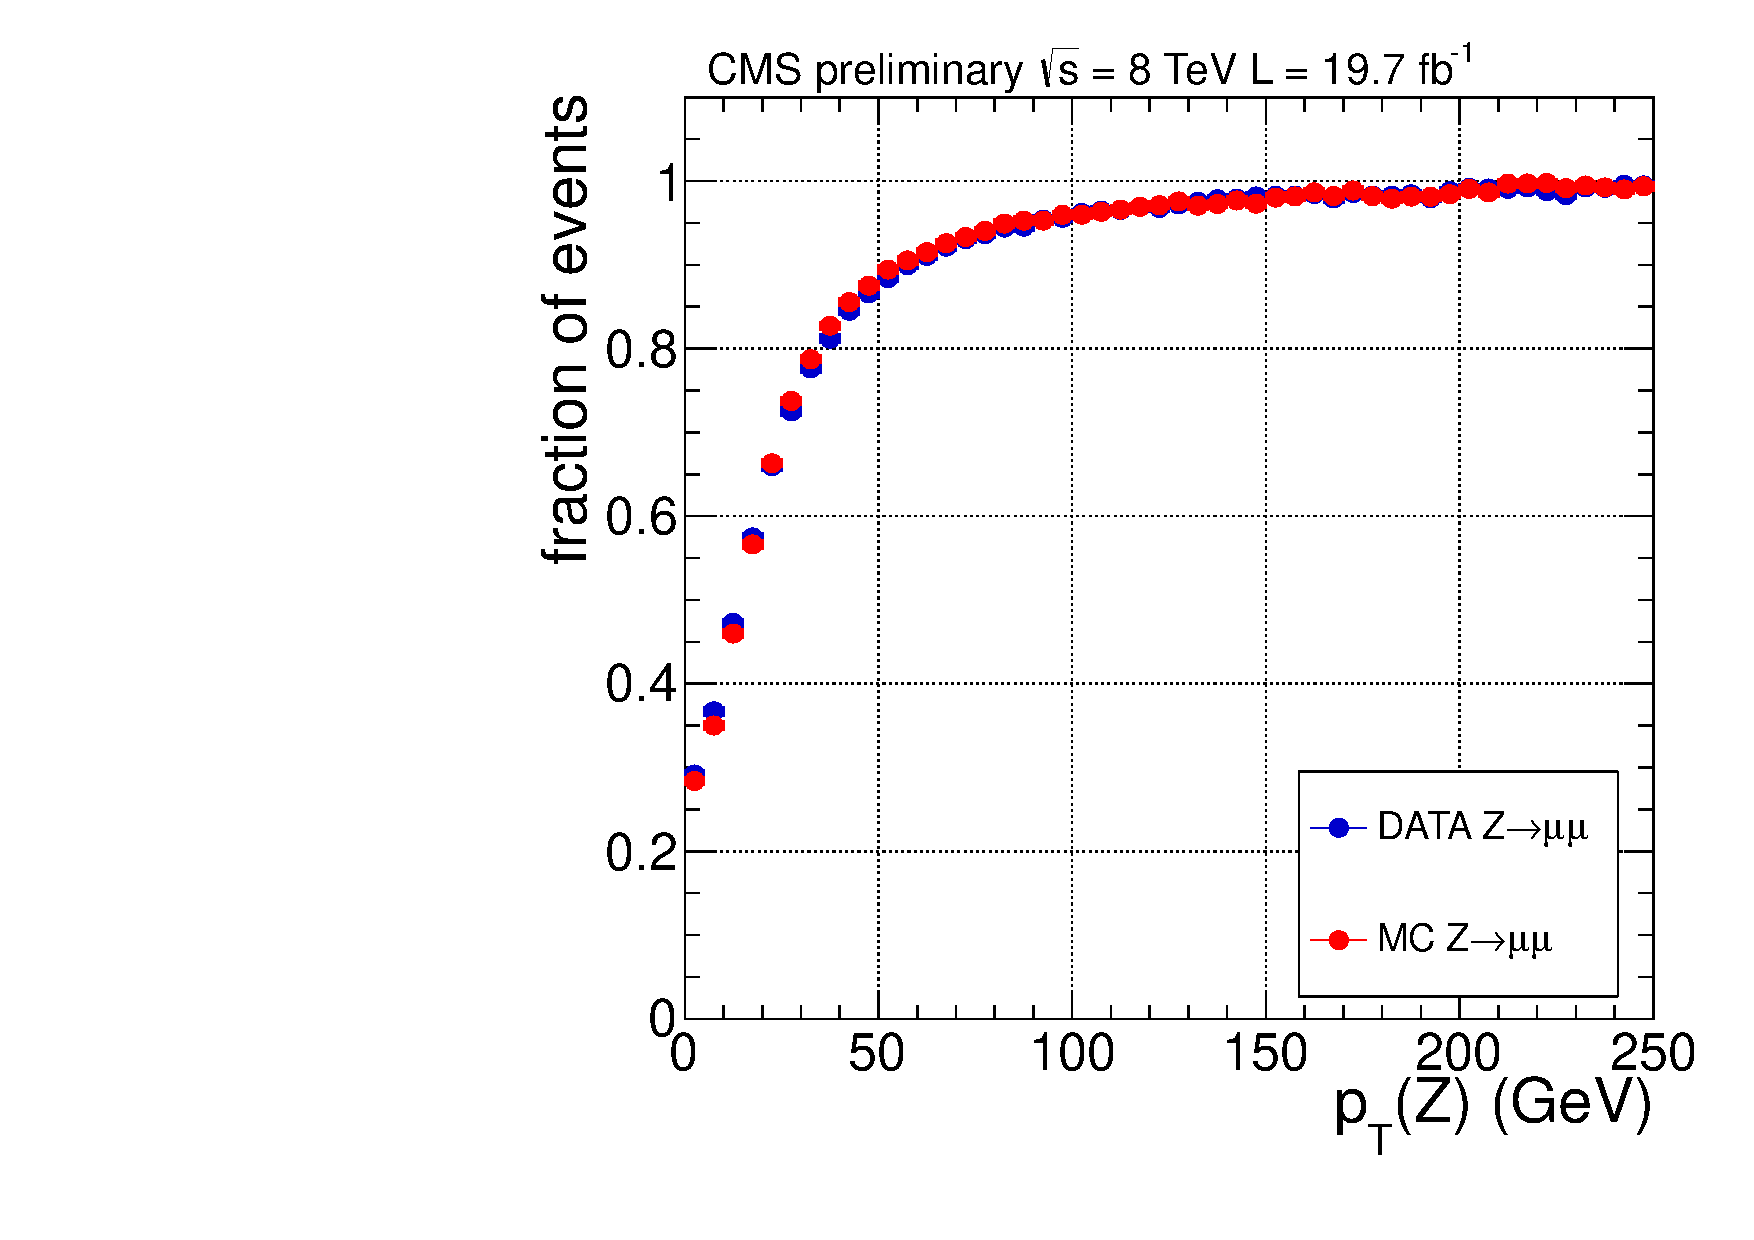
\includegraphics[width=0.48\textwidth]{ch3_comm_anal_comps/plots/vertex_bdt_efficiency_pt_8TeV.pdf}
  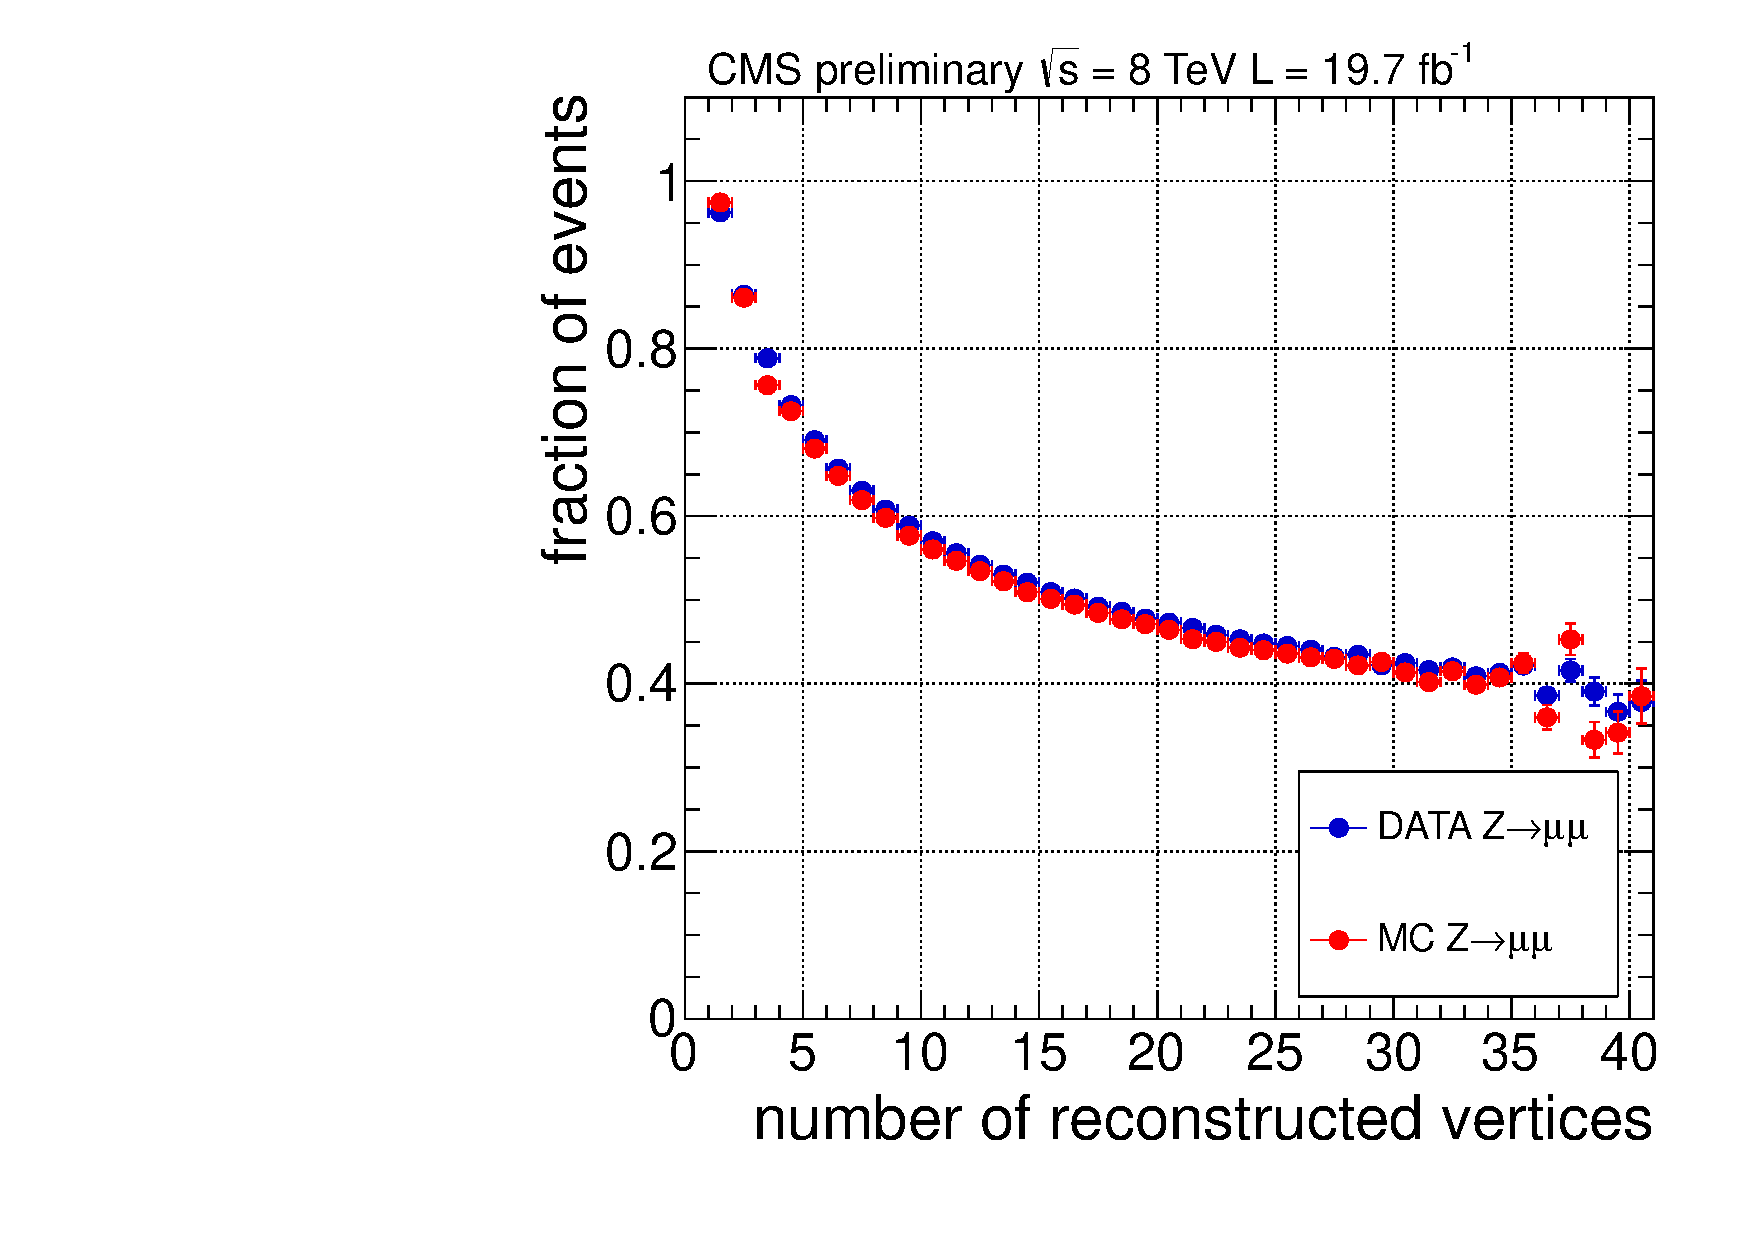
\includegraphics[width=0.48\textwidth]{ch3_comm_anal_comps/plots/vertex_bdt_efficiency_nvtx_8TeV.pdf} 
  \caption{The chosen vertex efficiency as measured in \Zmumu data and \MC as a function of $Z$ \pT (left) and number of reconstructed vertices (right) for the 7~TeV (top row) and 8~TeV (bottom row) data samples.}
  \label{fig:vertex_bdt_efficiency}
\end{figure}

\subsection{Estimating the per-event probability that the correct vertex is chosen}
\label{sec:bdt_prob}

The total efficiency of assigning the correct vertex using the method described in the preceeding section is at the level of 75\% during 2012 running conditions, where the correct vertex is defined as being within 10~mm of the true vertex. This means that for around 25\% of preselected events the mass resolution is dominated by the vertex resolution. Consequently, it is important to ascertain the probability that the chosen vertex is the correct one. An additional specific \BDT is constructed to address exactly this topic. The input variables used for this \BDT are:

\begin{itemize}
  \item The \pT of the diphoton system
  \item The number of vertices in each event
  \item The value of the per-vertex \BDT described above
  \item The $z$ distance, $\Delta z$, between the chosen vertex and the second and third choice vertices.
  \item The number of photon conversions used, either 0, 1 or 2.
\end{itemize}

There is a linear relation between the response of this \BDT and the correct vertex efficiency (or probability). This relationship is demonstrated in Figure~\ref{fig:vertex_bdt_prob} and is fitted with a single parameter straight line in order to analytically obtain the per-event correct vertex probability for a given event. Figure~\ref{fig:vertex_bdt_prob_efficiency} shows that this estimation reproduces the required vertex efficiency as a function of Higgs \pT and number of reconstructed vertices.

\begin{figure}
  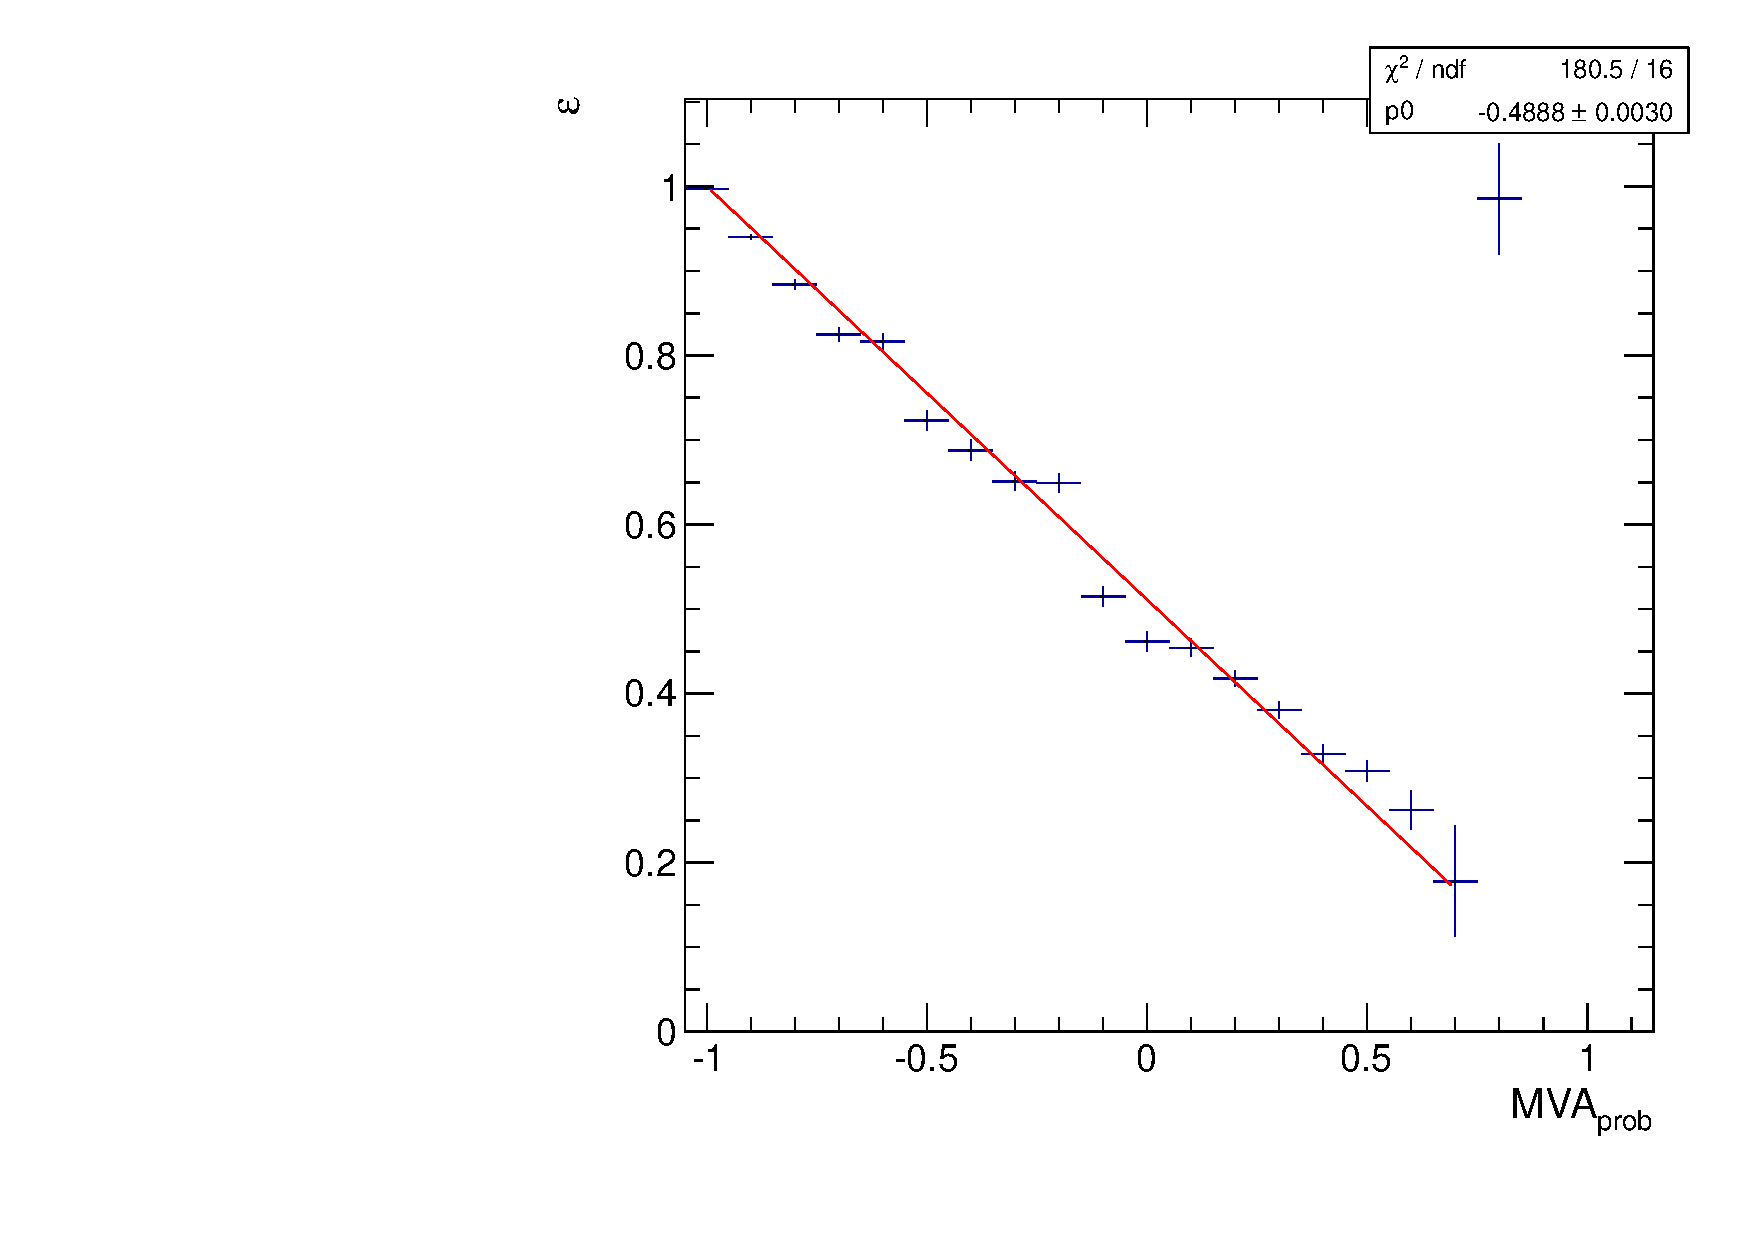
\includegraphics[width=0.48\textwidth]{ch3_comm_anal_comps/plots/vertex_bdt_prob.pdf}
  \caption{A demonstration of the linearity relation between the per-event vertex probability \BDT output distribution and the correct vertex probability}
  \label{fig:vertex_bdt_prob}
\end{figure}

\begin{figure}
  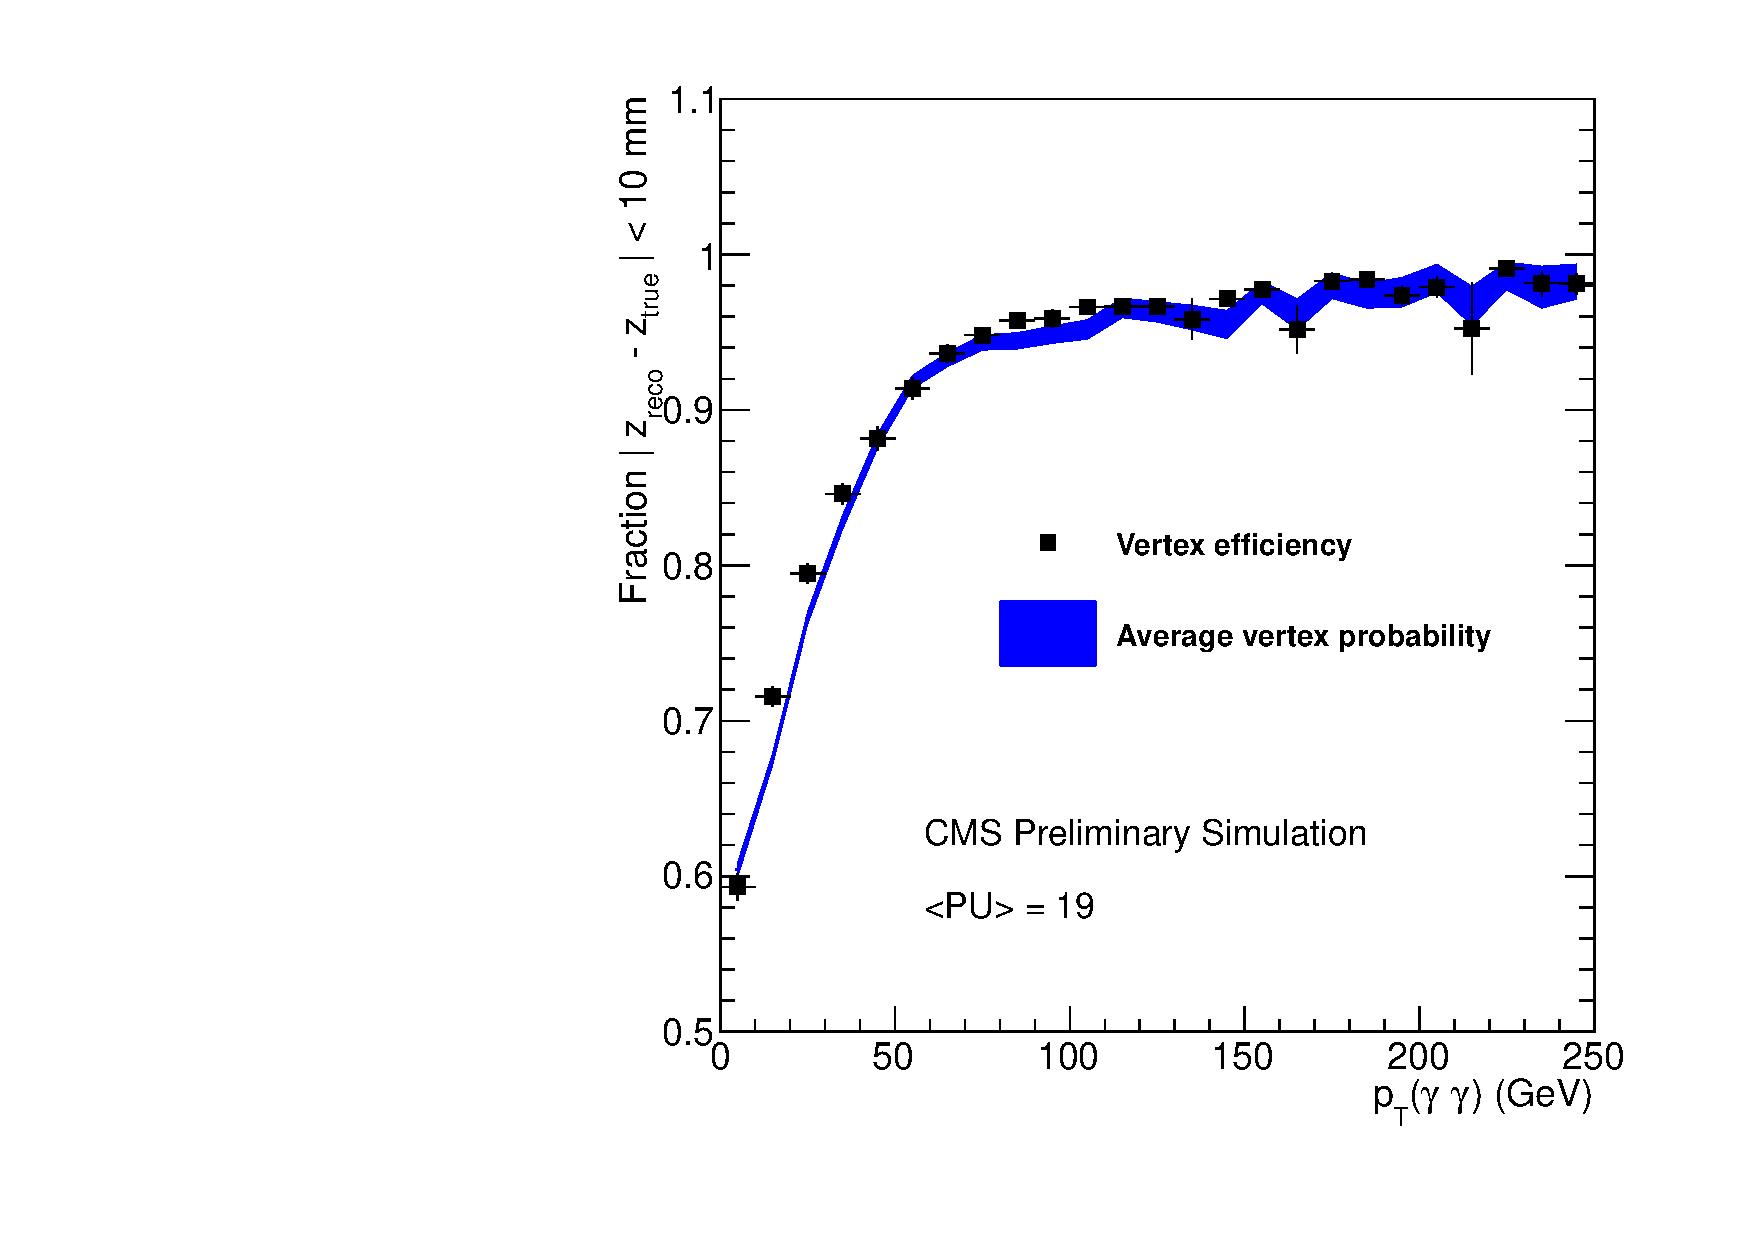
\includegraphics[width=0.48\textwidth]{ch3_comm_anal_comps/plots/vertex_bdt_prob_efficiency_pt.pdf}
  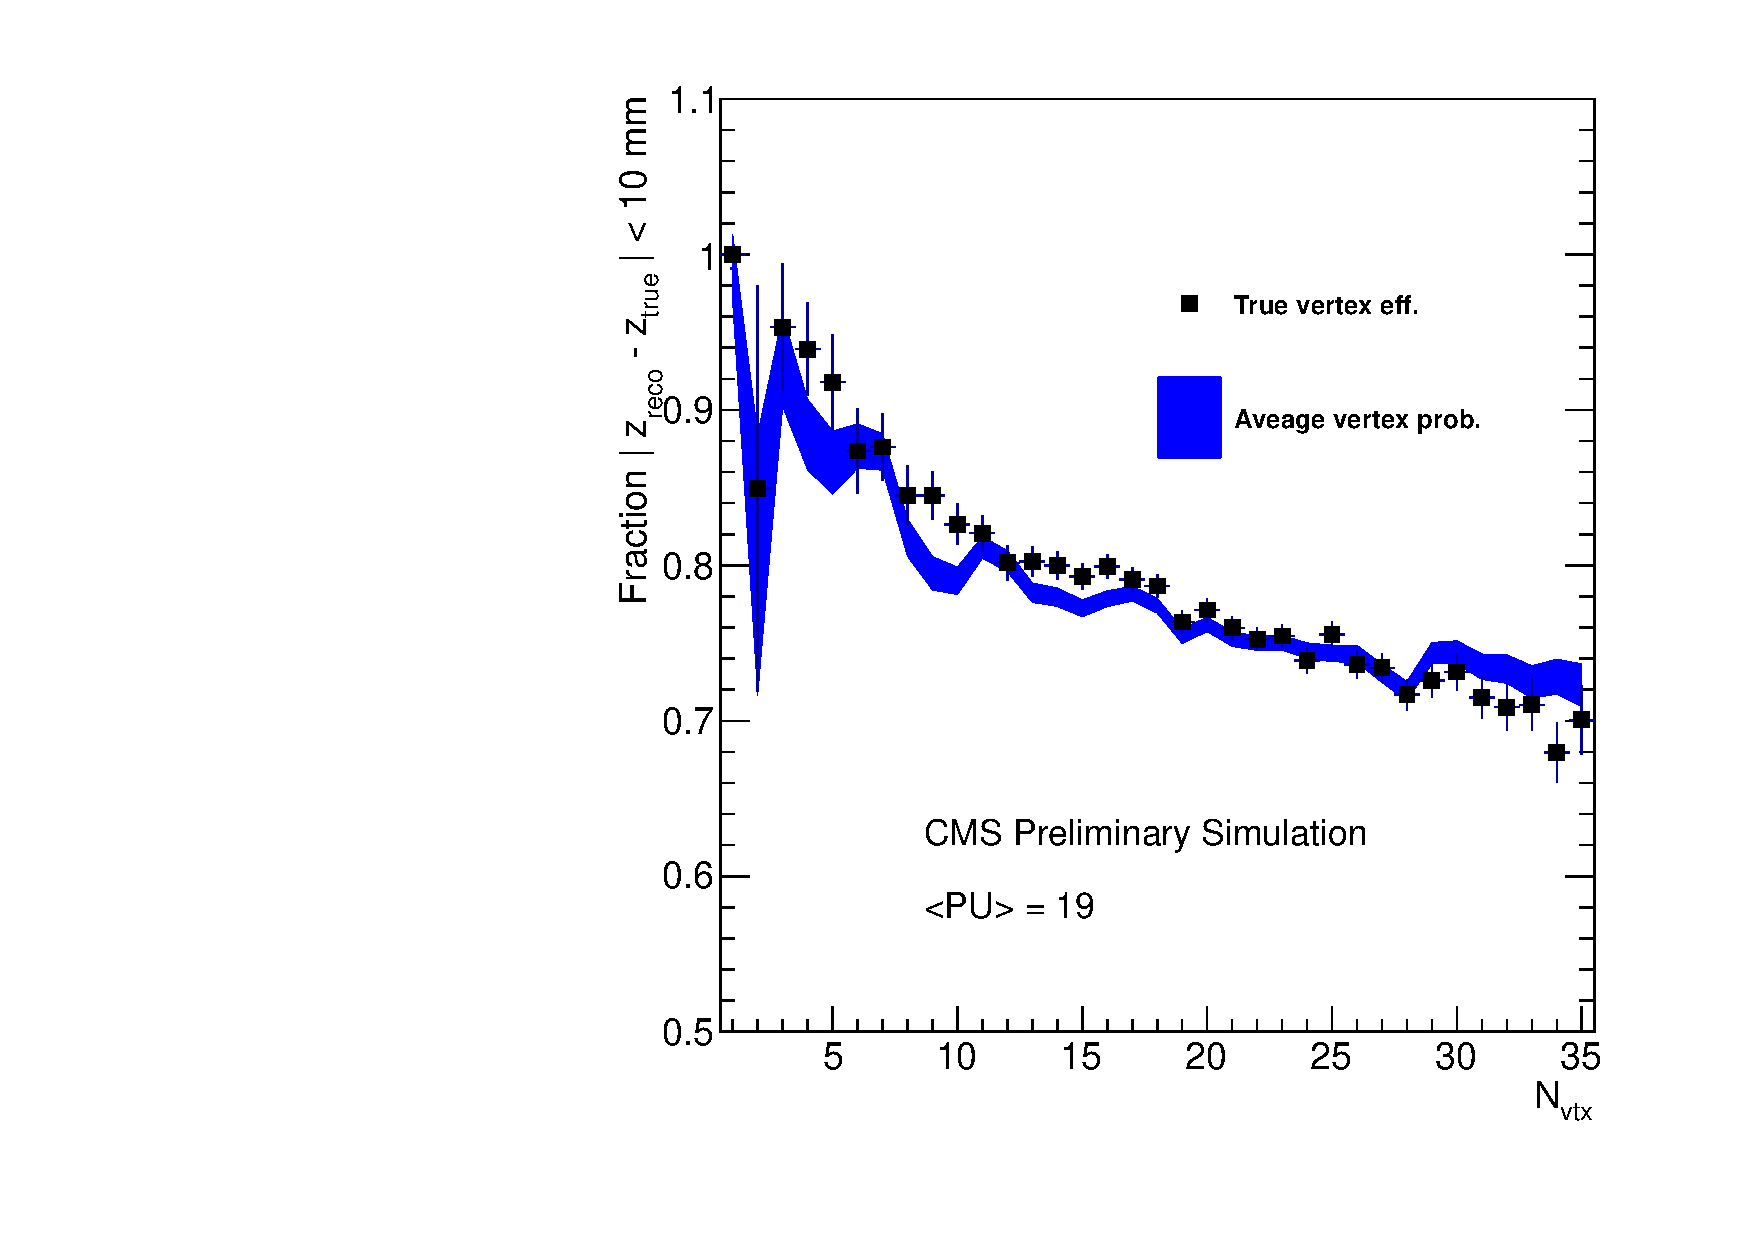
\includegraphics[width=0.48\textwidth]{ch3_comm_anal_comps/plots/vertex_bdt_prob_efficiency_nvtx.pdf}
  \caption{A comparison of the true vertex efficiency (black points) and the average vertex probability (blue band) a statistically independent \MC Higgs sample simulated with 2012 running conditions.}
  \label{fig:vertex_bdt_prob_efficiency}
\end{figure}

\section{Event preselection}
\label{sec:photon_presel}

A simple and loose preselection is applied to all photons before entering the analysis. The preselection requirements are identical for all analysis approaches and are designed to remove some \emph{fake} photons whilst mainting near 100\% trigger efficiency. The variables used for preselection are defined below and the preselection cuts are described in Table~\ref{table:preselection}.

\begin{itemize}
  \item $H/E$ - \textbf{The ratio of hadronic energy in the \HCAL tower behind the supercluster to the electromagnetic energy in the supercluster}. Neutral jets which fake photons typically leave a fraction of their energy in the \HCAL so there is a requirement that the value of this variable is small.
  \item $\sigma^{2}_{i\eta i\eta}$ - \textbf{The RMS spread of the shower in the eta direction}. Multiple showers of a \pizero, or more than one \pizero, result in a wider shower in \eta (as the \pizero decay product photons are separated in space). This cannot be exploited in the \phi direction because conversion electrons get separated by the magentic field, however in \eta single photons, even when converted, occupy a narrow region. The separation of the two photons from a \pizero is minimal when they share the energy eqaully and given that typically $p_{T}>>m_{\pi}$ the separation is close to minimal for most. Taking the transverse plane in the barrel, the separation $d=2Rm_{\pi}/p_{T}$ (where $R$ is the radius of the barrel), which for $p_{T}=40$GeV gives a value of $d=$8mm$\sim0.006\eta$. By refering to Table~\ref{tab:preselection} it is clear that the preselection requirement is quite loose.
  \item $ISO_{ECAL}$ - \textbf{The total \rho corrected electromagnetic energy in a cone of radius 0.4 in (\eta,\phi) around the photon candidate} - see Sec.~\ref{sec:iso}
  \item $ISO_{HCAL}$ - \textbf{The total \rho corrected hadronic energy in a cone of radius 0.4 in (\eta,\phi) around the photon candidate} - see Sec.~\ref{sec:iso}
  \item $ISO_{Tracks}$ - \textbf{The total \rho corrected track energy in a cone of radius 0.4 in (\eta,\phi) around the photon candidate} - see Sec.~\ref{sec:iso}
  \item $ISO_{PFCh}$ - \textbf{The total \rho corrected particle flow charged hadron energy in a cone of radius 0.4 in (\eta,\phi) around the photon candidate} - see Sec.~\ref{sec:iso}
\end{itemize}

In addition to the above an electron veto is applied to prevent contamination of the photon sample with electrons which originate from Drell Yan decays. This is acheived by removing photon candidates whose supercluster is matched to an electron track which has no missing hits in the innermost tracking region.

\begin{table}
\noindent
  \begin{center}
  \caption{Preselection cut values.}
    \begin{tabular}{c c c c c c c c c c c }
                & \multicolumn{2}{c}{Barrel} & \multicolumn{2}{c}{Endcap} \\ 
      \hline
      R9        & $H/E$ & $\sigma^{2}_{i\eta i\eta}$ & $HoE$ & $\sigma^{2}_{i\eta i\eta}$  \\ 
      $\le$ 0.9 & $<$ 0.075 & $<$ 0.014 & $<$ 0.075 & $<$ 0.034 \\
      $>$ 0.9   & $<$ 0.082 & $<$ 0.014 & $<$ 0.075 & $<$ 0.034  \\ 
      \hline    
                & \multicolumn{4}{c}{Both Barrel and Endcap}\\ 
      \hline
      R9        & $ISO_{ECAL}$ & $ISO_{HCAL}$ &  $ISO_{Tracks}$ & $ISO_{PFCh}$ \\ 
      $\le$ 0.9 &$<$ 4 GeV & $<$ 4 GeV & $<$ 4 GeV & $<$ 4 GeV\\ 
      $>$ 0.9   &$<$ 50 GeV & $<$ 50 GeV & $<$ 50 GeV & $<$ 4 GeV\\ 
    \end{tabular}
  \label{table:preselection}
  \end{center}
\end{table}

\section{Using $Z$ decays for validation and efficiency measurements}
\label{sec:zee}

Whilst no known ``standard candles" with high statistics exist for high \pT photons in the \LHC environment a powerful control source for the \Hgg decay in both data and \MC is the \Zee decay. From a detector view point electrons are very similar to photons and the $Z$ is relatively near the relevant Higgs search range in mass. The differences between the $Z$ and the Higgs, in both their mass and \pT distribution, and also the differences between electrons originating from a $Z$ and photons originating from a Higgs are important systematic uncertainties on the Higgs mass scale and resolution. By inverting the electron veto usually applied in the preselection the Higgs to two photon analysis can be identically replicated but the very pure diphoton sample replaced with a pure dielectron sample. One additional process which can be used as a direct control for photons is the \Zmumugamma decay although the statistics, even with the LHC luminosity, are very low. Many of the input variables used in training the \BDTs and cuts are validated with both \Zee and \Zmumugamma data/\MC comparison plots. An example is shown in Figure~\ref{fig:dielectronmass} for the reconstructed di-electron mass for events passing the preselection described in Table~\ref{table:preselection}.

As previously shown (in Sec.~\ref{sec:scale_smearing}) data/\MC comparison of the \Zee decay are used to derive scale corrections for the data and smearing of the \MC. Discrepancies between data and \MC in \Zee decays of important analysis variables are accounted for by introducing systematic uncertainties to cover them. In addition the ``tag and probe" method ~\cite{tag_and_probe} is used on \Zee decays to evaluate the signal efficiency for the preselection and analysis cuts. Several stages of the analysis are validated in this way and where appropriate systematic uncertainties are included to account for any data/\MC differences. Although the numbers and uncertainties themselves are derived from \Zee samples (because of the much higher statistics), they are always cross checked with the \Zmumugamma sample.

\begin{figure}
  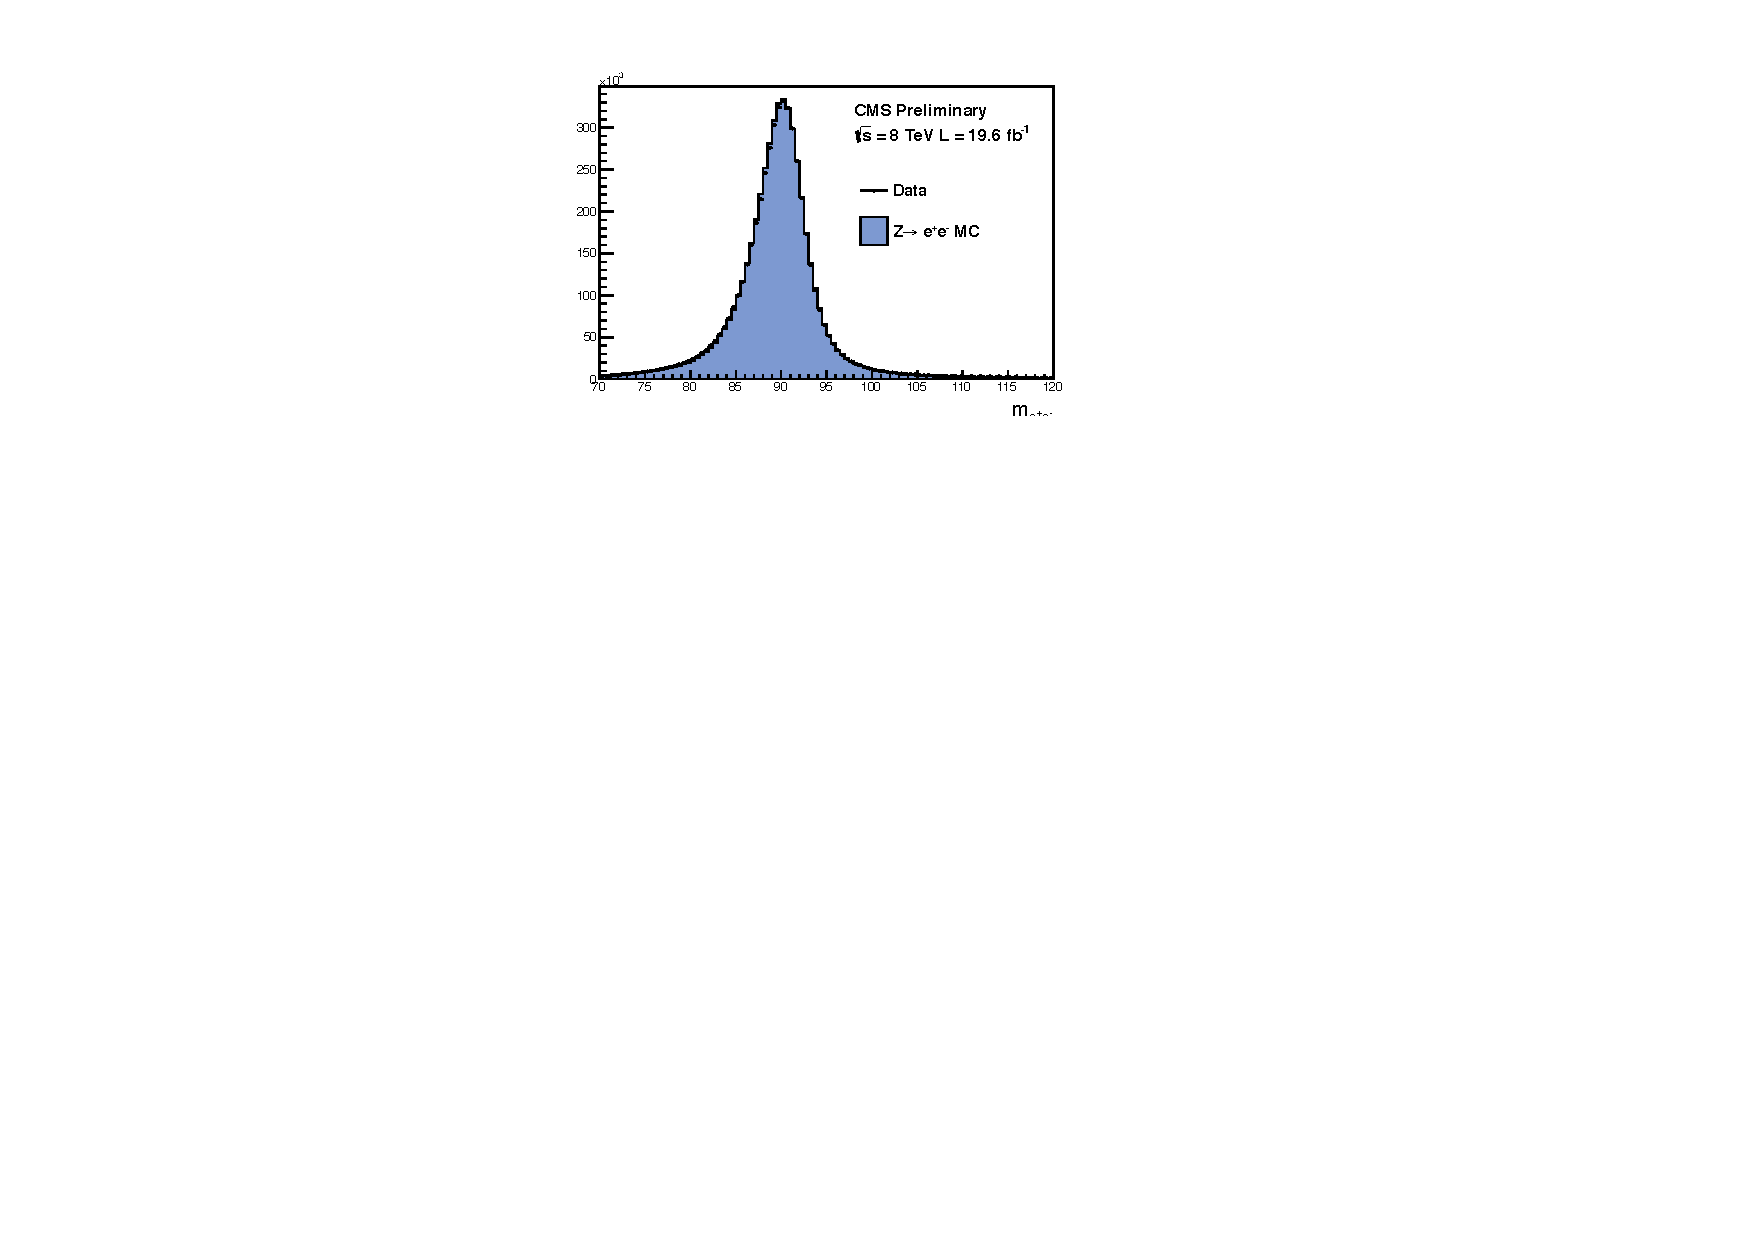
\includegraphics[width=0.48\textwidth]{ch3_comm_anal_comps/plots/zee_mass.pdf}
  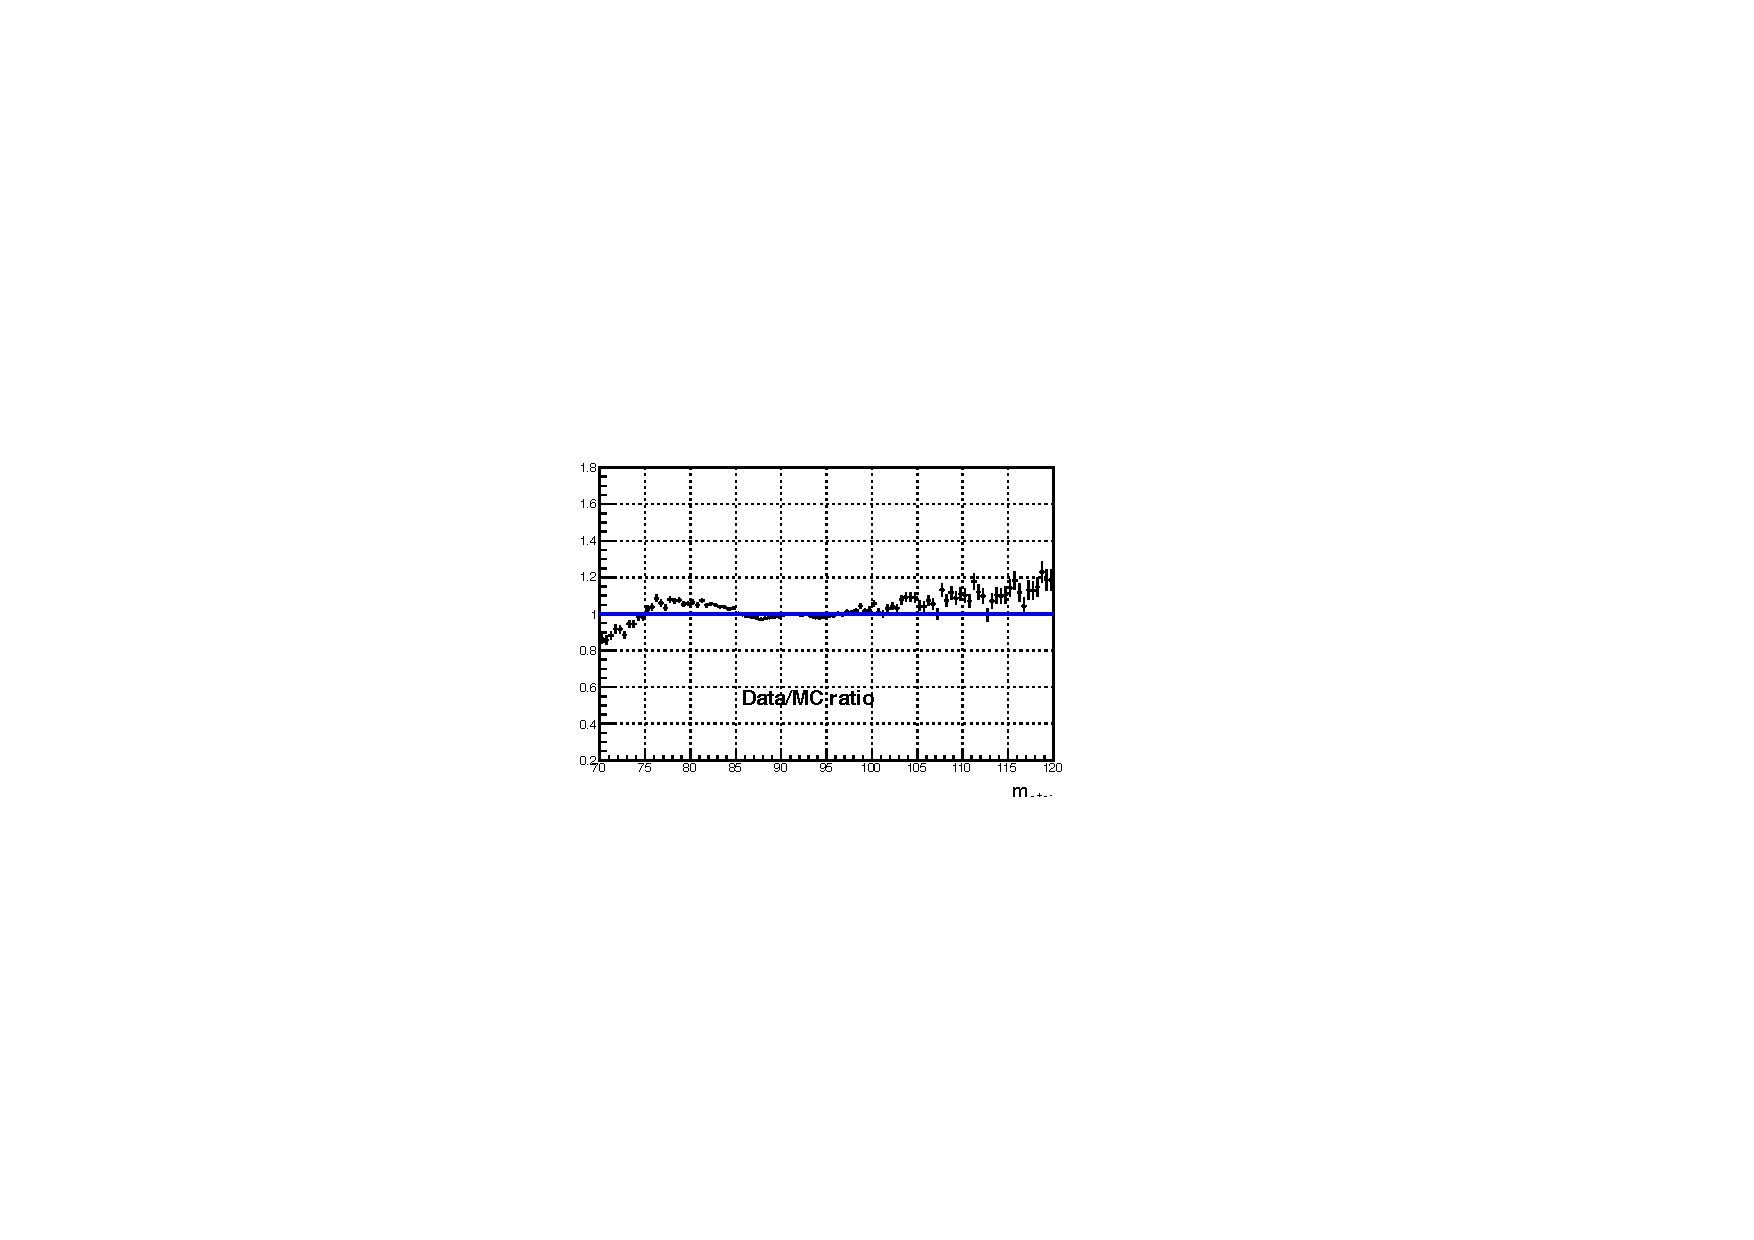
\includegraphics[width=0.48\textwidth]{ch3_comm_anal_comps/plots/zee_mass_ratio.pdf}
  \caption{The di-electron mass distribution after applying the preselection (described in Sec.~\ref{sec:photon_presel}) and the scale and smearing corrections (described in Sec.~\ref{sec:scale_smearing}) whilst inverting the electron veto. The left plot shows the data at 8TeV as the black points with the Drell Yan \MC sample as the blue histogram. The Data/\MC ratio is shown in the right hand plot. \red{Plot needs updating}}
  \label{fig:dielectronmass}
\end{figure}

  \chapter{Selection and Categorisation}
\label{chap:selection_and_categorisation}
\chapterquote{Science never solves a problem without creating ten more.}
{George Bernard Shaw, 1856 -- 1950}

\section{Description}

A description of the selection and categorisation under two schemes � a robust cut-based driven approach (used later for the spin) and a highly optimized, standard model specific multivariate method (used later for the nominal analysis and the sideband background method). This would also include the validation procedure with Z->ee decays.

\textbf{15 pages}

\textbf{Brief outline of the three analyses being discussed and their uses}

This thesis presents results of three different analyses used in the Higgs to two photon search at CMS. The first, the \acf{CiC} analysis, is designed for simplicity and robustness as a cut based approach used to cross check the main result and, owing to it's low level of model dependence, for the spin analysis. The other two are more aggressive multivariate methods optimised specifically to search for a \ac{sm} Higgs boson. The first of these has a fully parametric definition of the diphoton invariant mass spectrum and as such is know as the \acf{MFM} or \acf{MBM} analysis. The second serves to cross check the background, the most significant unknown in a search like this, by extracting the background under the signal region from sidebands in the diphoton invariant mass spectrum, referred to as the \acf{SMVA}.

% ---- SECTION ----
\section{Photon selection}
\label{sec:pho_selection}
  
  \subsection{Selection using cuts in categories}
  \label{sec:cic}

  \subsection{Photon ID MVA}
  \label{sec:pho_id_mva}
  
  \subsection{Diphoton event level MVA}
  \label{sec:diphoton_bdt}

% ---- SECTION ----
\section{Event categorisation}
\label{sec:categorisation}

  \subsection{Exclusive mode tagging}
  \label{sec:exclusive_tags}

  \subsection{Inclusive mode categorisation in the mass factorised analysis}
  \label{sec:inclusive_cats_massfac}

  \subsection{Inclusive mode categorisation in the sideband analysis}
  \label{sec:invlusive_cats_sideband}

% ---- SECTION ----
\section{Signal modelling}
\label{sec:signal_model}

  \subsection{Mass factorised analysis}
  \subsection{Sideband analysis}

% ---- SECTION ----
\section{Background modelling}
\label{sec:background_model}

  \subsection{Mass factorised analysis}
  \subsection{Sideband analysis}

% ---- SECTION ----
\section{Systematic Uncertainties}
\label{sec:systematics}

  \chapter{Analysis and Results}
\label{chap:results}
\chapterquote{I'm a bus}
{Darren Burton 1987--2013}

\section{Description}

This would include a detailed description of the signal and background models used and the systematics included. I would describe the statistical tools used such as hypothesis testing with a test statistic and show the results which would include exclusion limits, pvalues and SM best fit parameters (mass, signal strength, couplings etc.). One of the important considerations of the Hgg analysis is the estimation of the background. This second part of this section will concentrate on presenting an alternate analysis which takes a completely different approach to modeling the background and cross-checks the result above.

\section{Statistics}
\subsection{Use of the Likelihood function as a test statistic}

\section{Results of the mass factorised analysis}

\section{Results of the sideband analysis}

  \chapter{Spin Analysis}
\label{chap:spin}
\chapterquote{In a spin, loving the spin I'm in.}{Louis Prima, 1910--1978}

The Landau-Yang theorem forbids the direct decay of a spin-1 particle into a pair of photons~\cite{Landau1948,Yang1950}. 
Consequently the spin analysis compares the expectation of the spin-0 SM Higgs, \zerop, and the spin-2 \emph{graviton-like} 
model with minimal couplings, \twomp,~\cite{Gao2010}. The \twomp graviton resonance is produced in one of two ways, gluon-fusion ($gg$) 
or quark-antiquark annihilation (\qqbar). We present hypothesis tests between the \zerop and the \twomp varying the the amount of 
\twomp production from \qqbar. For the \zerop SM 
resonance all production modes have been considered; gluon-fusion, vector-boson-fusion, W and Z boson associated production and top-antitop 
associated production. 

As the \twomp is just one of many spin-2 models we have attempted to make the analysis as model independent as possible. As a means of 
discriminating the two hypotheses we use the scattering angle in the Collins-Sopper frame, \costhetastar ~\cite{CollinsSoper1977}, which is defined as the angle, in the diphoton rest frame, between the collinear diphotons 
and the line which bisects one incoming beam with the negative of the other beam, 

\begin{equation}
  \cos(\theta^{\ast}_{\mbox{\tiny{CS}}}) = 2\times\frac{E_{2}p_{z1}-E_{1}p_{z2}}{m_{\gamma\gamma}\sqrt{m^{2}_{\gamma\gamma}+p^{2}_{T\gamma\gamma}}},
\end{equation}

where $E_{1}$ and $E_{2}$ are the energies of the leading and trailing photon, $p_{z1}$ and $p_{z2}$ are the $z$-component momenta 
of the leading and trailing photon and $m_{\gamma\gamma}$ and $p_{T\gamma\gamma}$ are the invariant mass and transerve momenta of the diphoton system.

In its rest frame the photons from the decay of a spin-0 boson are isotropic. Hence prior to acceptance cuts, the distribution of \costhetastar 
under the \zerop hypothesis is uniformly flat. In general this is not the case for spin-2 decays. 

In order to reduce any model dependence in the analysis the cut based photon selection, described in Sec.~\ref{sec:cic}, is used to pick events. The \MVA methods used for event selection in the nominal analysis use specific \SM \MC training samples and most importantly one of the training variables used, namely $\cos(\phi_{1}-\phi_{2})$, is highly correlated to the angular variable, \costhetastar, which can be used to distinguish spin hypotheses. Furthermore, given the unusual production modes of a spin-2 boson, no exclusive tagging is used in the spin analysis. The impact of using jet variables was studied but it was found that the sensitivty for distinguishing spin hypotheses was improved by a neglible amount.

Two statistical tests are carried out in the spin analysis:

\begin{enumerate}
  \item The signal strength, $\mu$, is extracted differentially in bins of \abscostheta. This is a relatively model independent test and in principal allows any spin model to be compared to the data.
  \item The statistical separation between different spin hypotheses is calculated using a test statistic similar to the one described in Sec.~\ref{sec:stats} and the $CL_{s}$ exclusion method. This is a highly model dependent but can allow the exclusion of specific spin models.
\end{enumerate}

\section{Event categorisation}
\label{sec:spin_cats}

%Preceding the cut based selection mentioned in section \ref{sec:photonID} and described in Ref.~\cite{HIG-13-001}, photons
%are preselected requiring, $p_{T}/m_{\gamma\gamma}>1/3$ ($p_{T}/m_{\gamma\gamma}>1/4$) for the leading (subleading) photon and
%$|\eta_{\mbox{\tiny{cluster}}}|<2.5$ for all photons, where $p_{T}$ is the transverse momentum of a photon, $m_{\gamma\gamma}$ is the diphoton invariant mass and $|\eta_{\mbox{\tiny{cluster}}}|$ is the pseudorapidity of the photon supercluster. In addition photons are rejected whose supercluster lies within the barrel-endcap transition region, $1.4442<|\eta_{\mbox{\tiny{cluster}}}|<1.566$.
The effect of the photon selection cuts on the distributions of 
\abscostheta is illustrated in Fig.~\ref{fig:acc_cuts}. Before any acceptance cuts, Fig.~\ref{fig:acc_cuts} (left), the \abscostheta
distribution of the \zerop processes is flat. This is not the case for the \twomp processes (gluon-fusion and quark-antiquark annihilation). After the selection cuts are applied these distributions are considerably distorted, Fig.~\ref{fig:acc_cuts} (right). As a Higgs produced from vector-boson-fusion, which is $\sim$8\% of the total (compared to $\sim$88\% from gluon fusion),  is typically produced at higher transverse momentum there is some additional contribution of \zerop signal at high values of \abscostheta compared to the \twomp production modes after the selection cuts.

\begin{figure}
	\begin{center}
	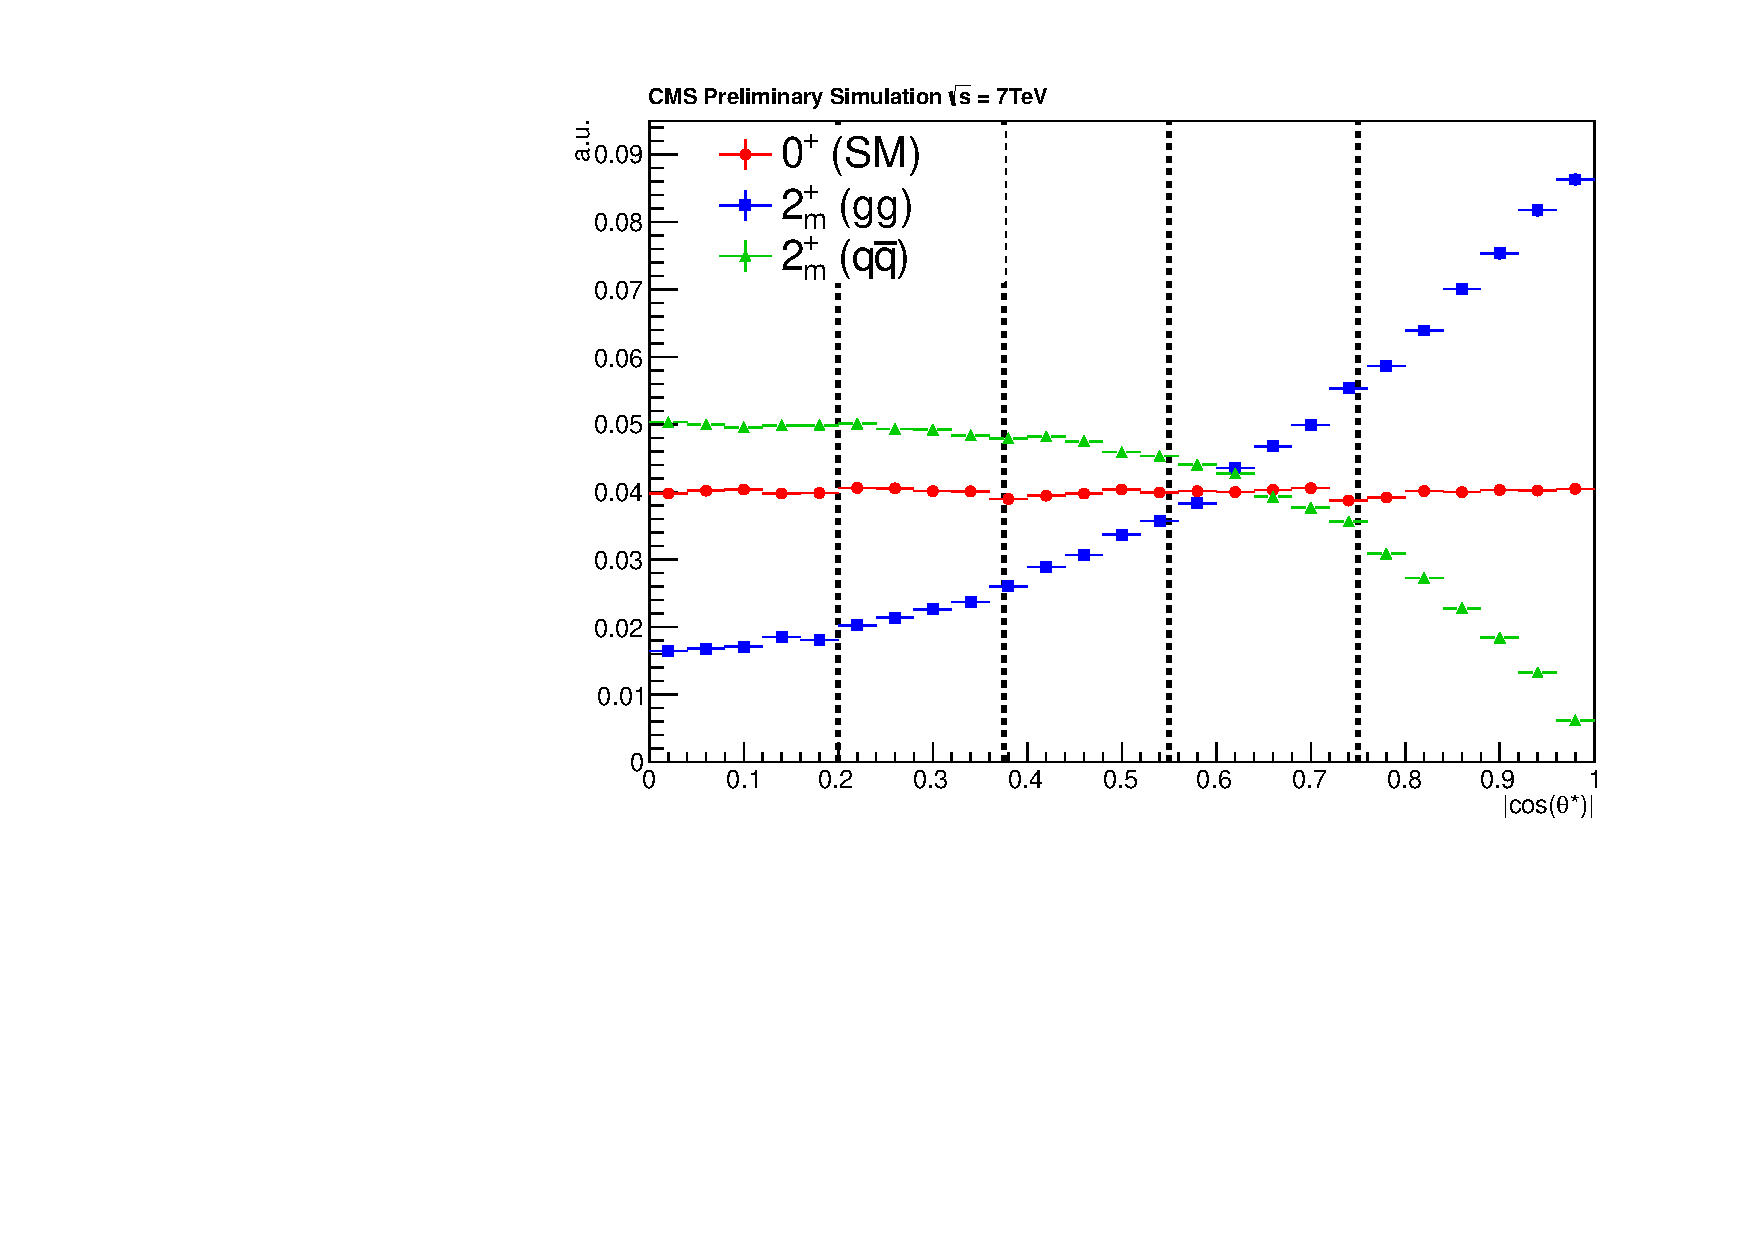
\includegraphics[width=0.49\linewidth]{ch6_spin_anal/plots/before_7TeV.pdf}
	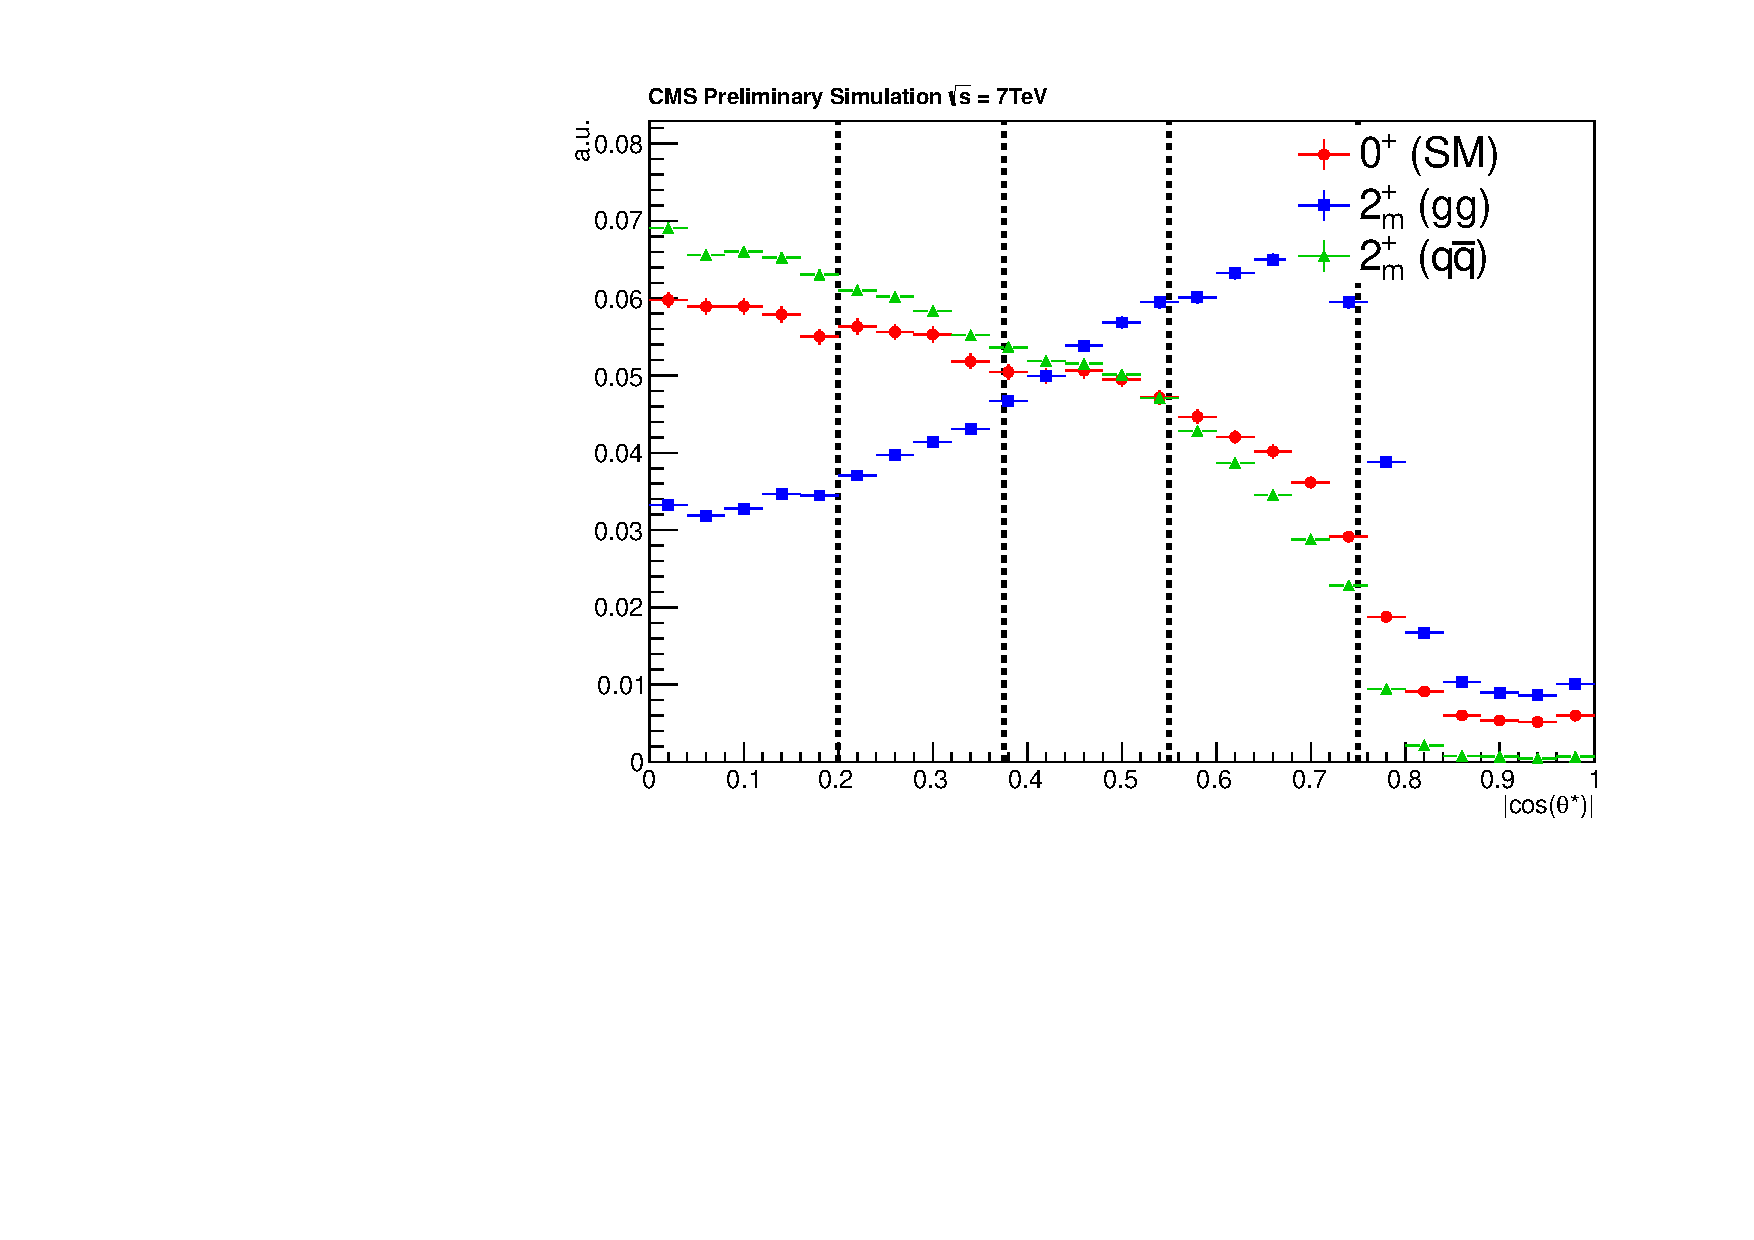
\includegraphics[width=0.49\linewidth]{ch6_spin_anal/plots/after_7TeV.pdf} \\
	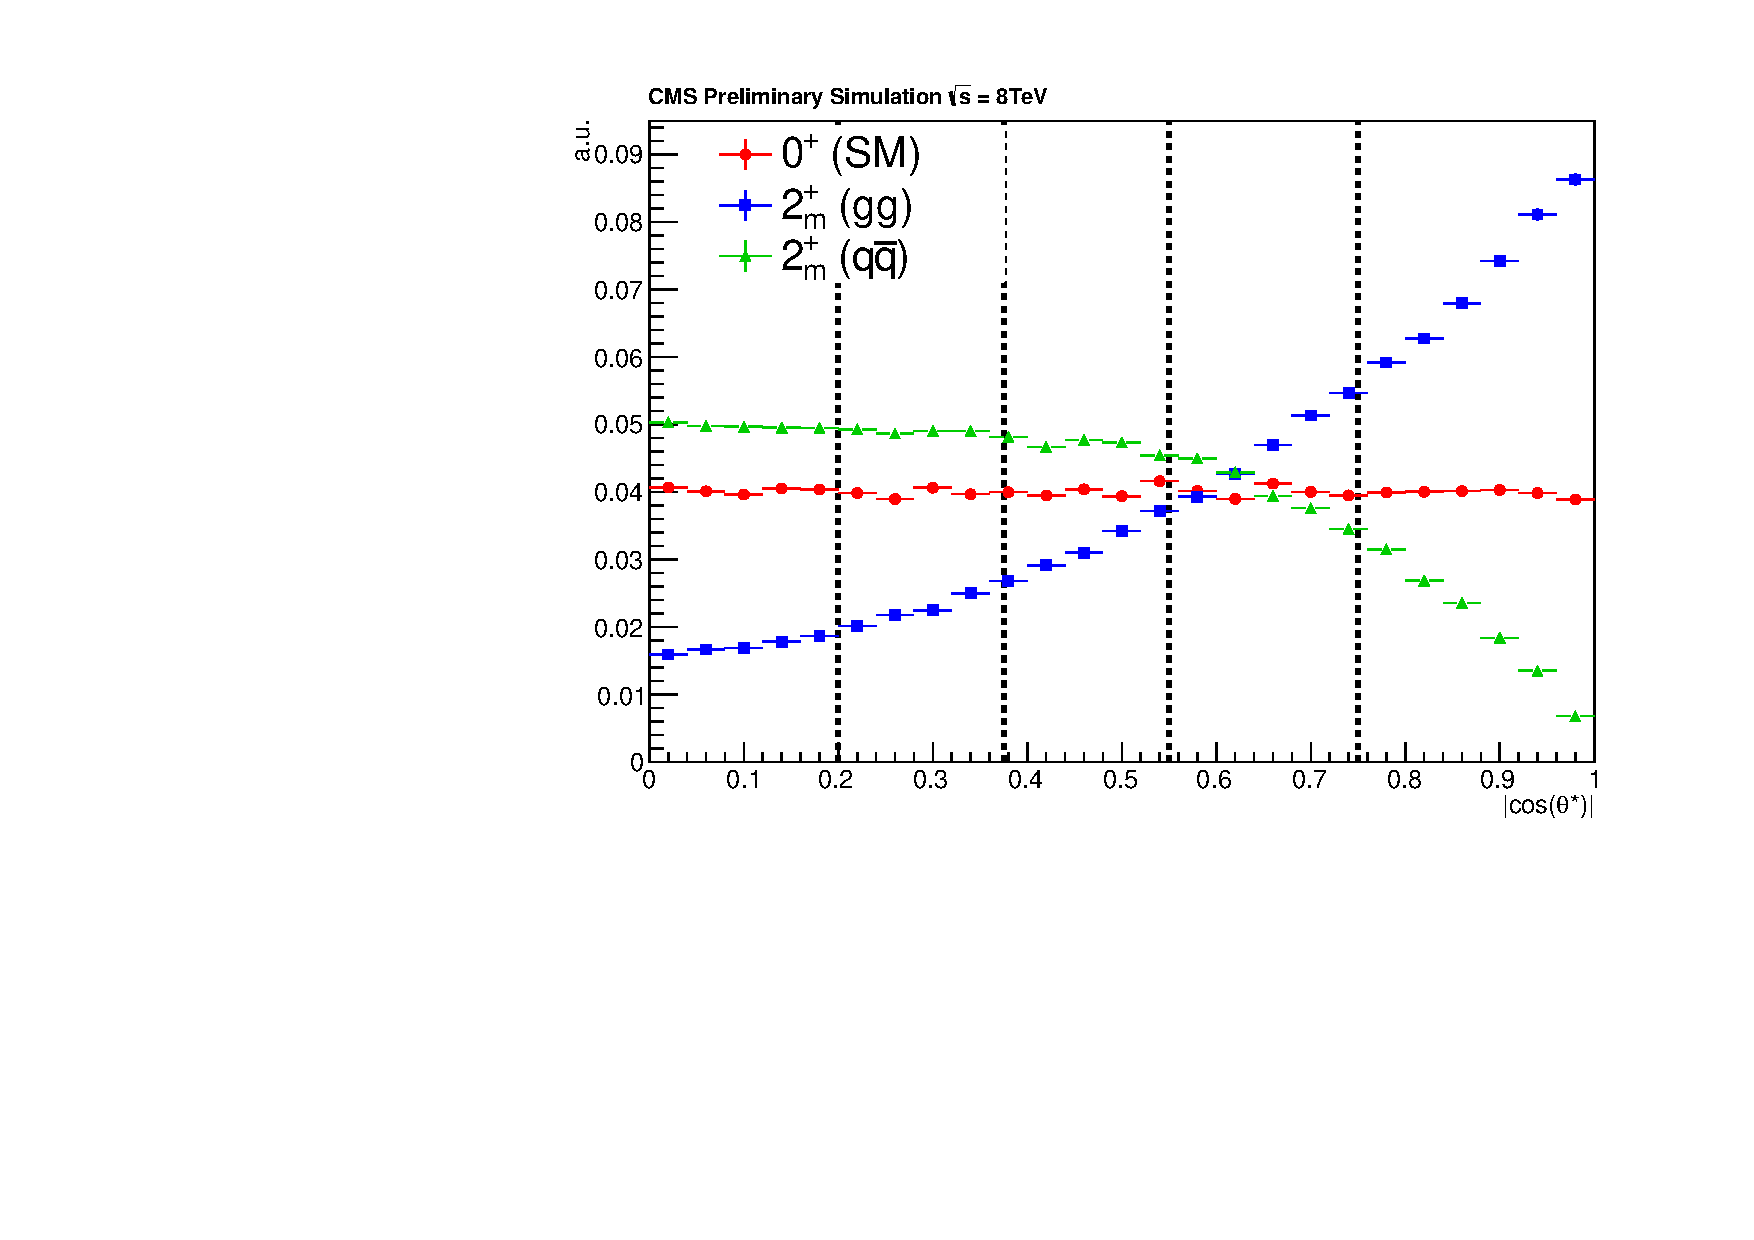
\includegraphics[width=0.49\linewidth]{ch6_spin_anal/plots/before_8TeV.pdf}
	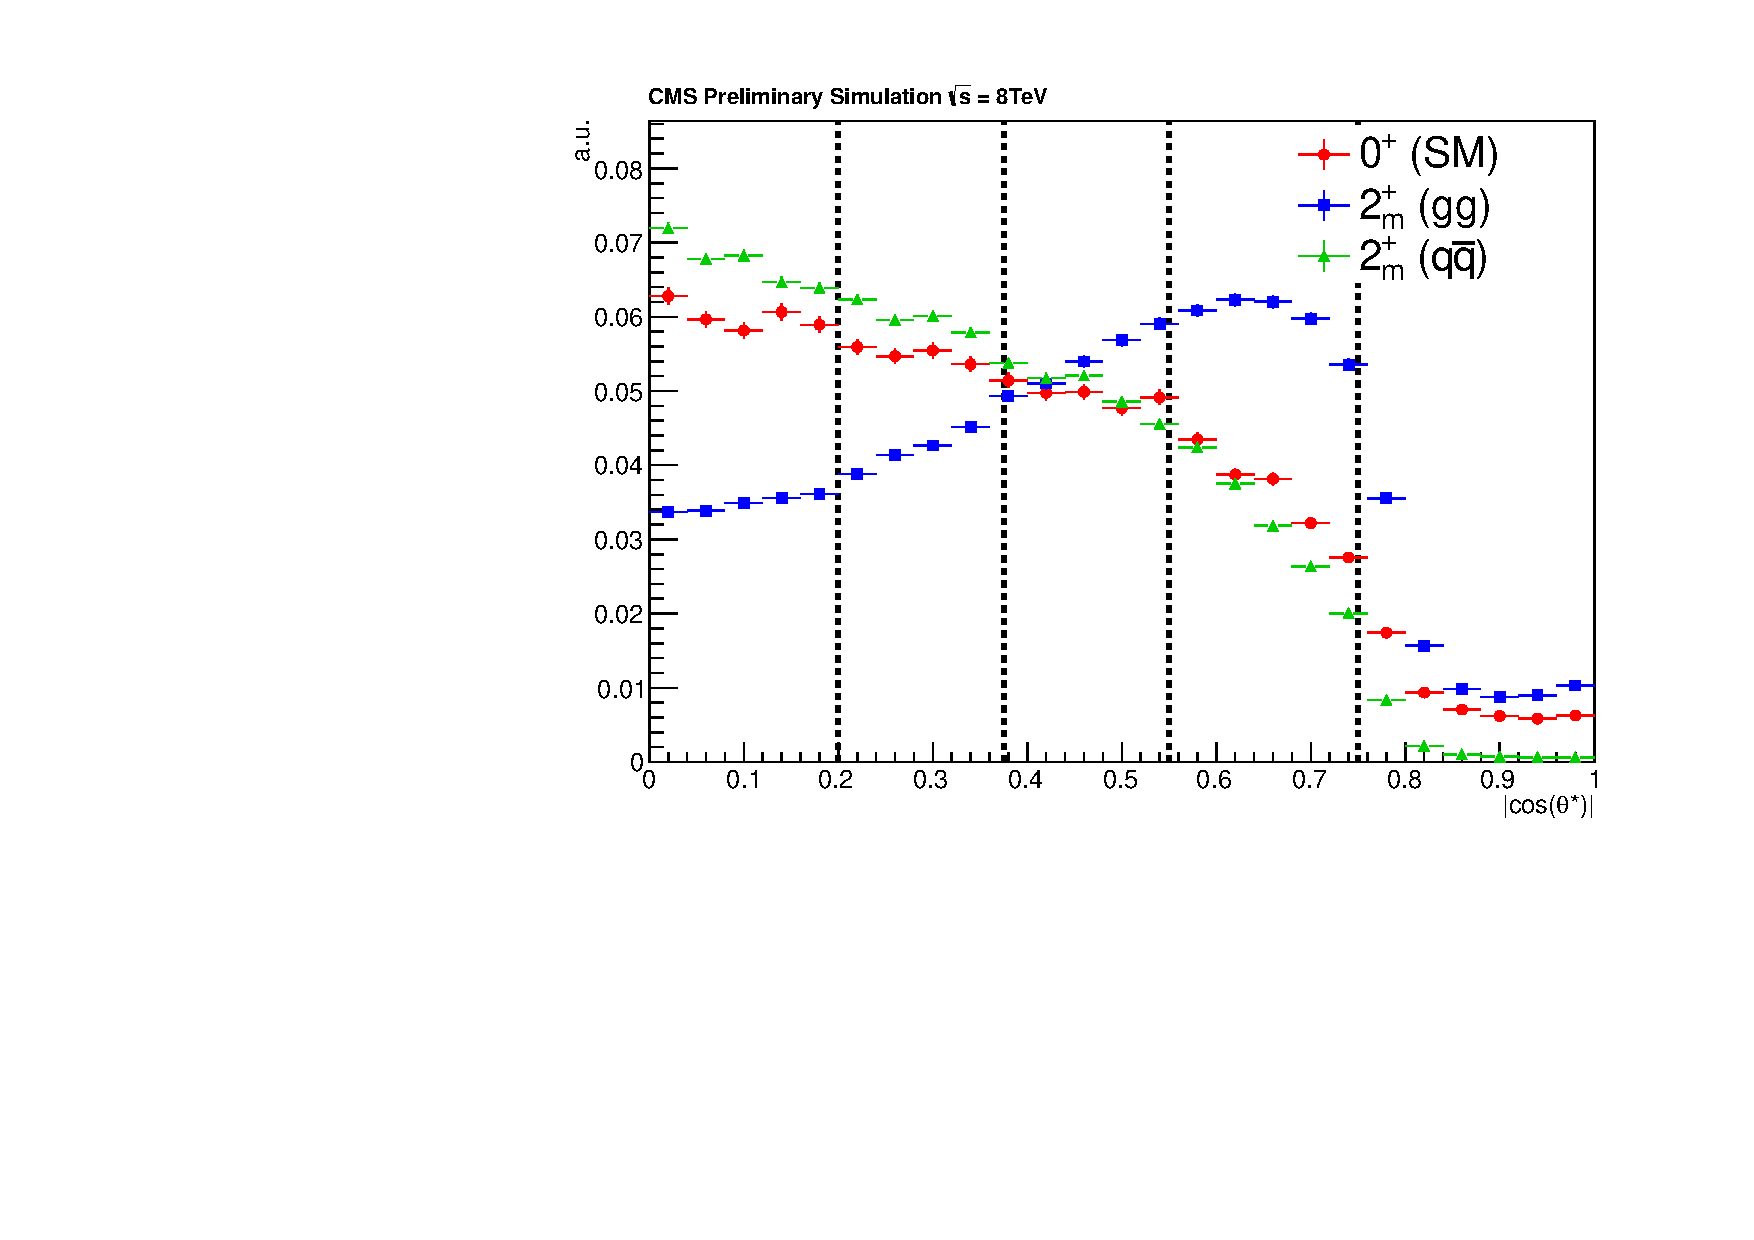
\includegraphics[width=0.49\linewidth]{ch6_spin_anal/plots/after_8TeV.pdf} \\
	\caption{The distribution of \abscostheta before any selection cuts (left) and after the selection cuts (right) for the 7~\TeV dataset top row and the 8~\TeV dataset bottom row. The three histograms represent the spin $0^+$ distribution with all SM production modes (red circular points), the spin $2^+_m$ distribution with the gluon-fusion production mode (blue square points) and the spin $2^+_m$ distribution with the quark-antiquark annihilation production mode (green triangular points). The \abscostheta category boundaries are shown as the black dashed lines.}
	\label{fig:acc_cuts}
	\end{center}
\end{figure}	

A robust analysis is possible because although the acceptance $\times$ efficiency varies considerably as a function of \abscostheta, the shape of this variation is largely independent of the spin-parity model. This is also true in restricted ranges of $\eta$ and $R_{9}$ which allows us to extract the signal yield in bins of \abscostheta in a comparatively model independent way. 
Figure~\ref{fig:eff_acc} shows the efficiency $\times$ acceptance ratio between the \twomp (with gluon-fusion production only) and \zerop (all SM production modes) as a function of \abscostheta in the $|\eta|$ and $R_{9}$ categories defined in Table~\ref{table:cats1}. It is clear that the acceptance $\times$ efficiency between the spin-0 and spin-2 models is independent of \abscostheta apart from at high values of \abscostheta where the vector-boson-fusion production in the SM plays a role. This motivates the choice of \abscostheta category boundaries described below where all the categories have similar efficiency $\times$ acceptance apart from the bin highest in \abscostheta.

\begin{figure}
	\begin{center}
	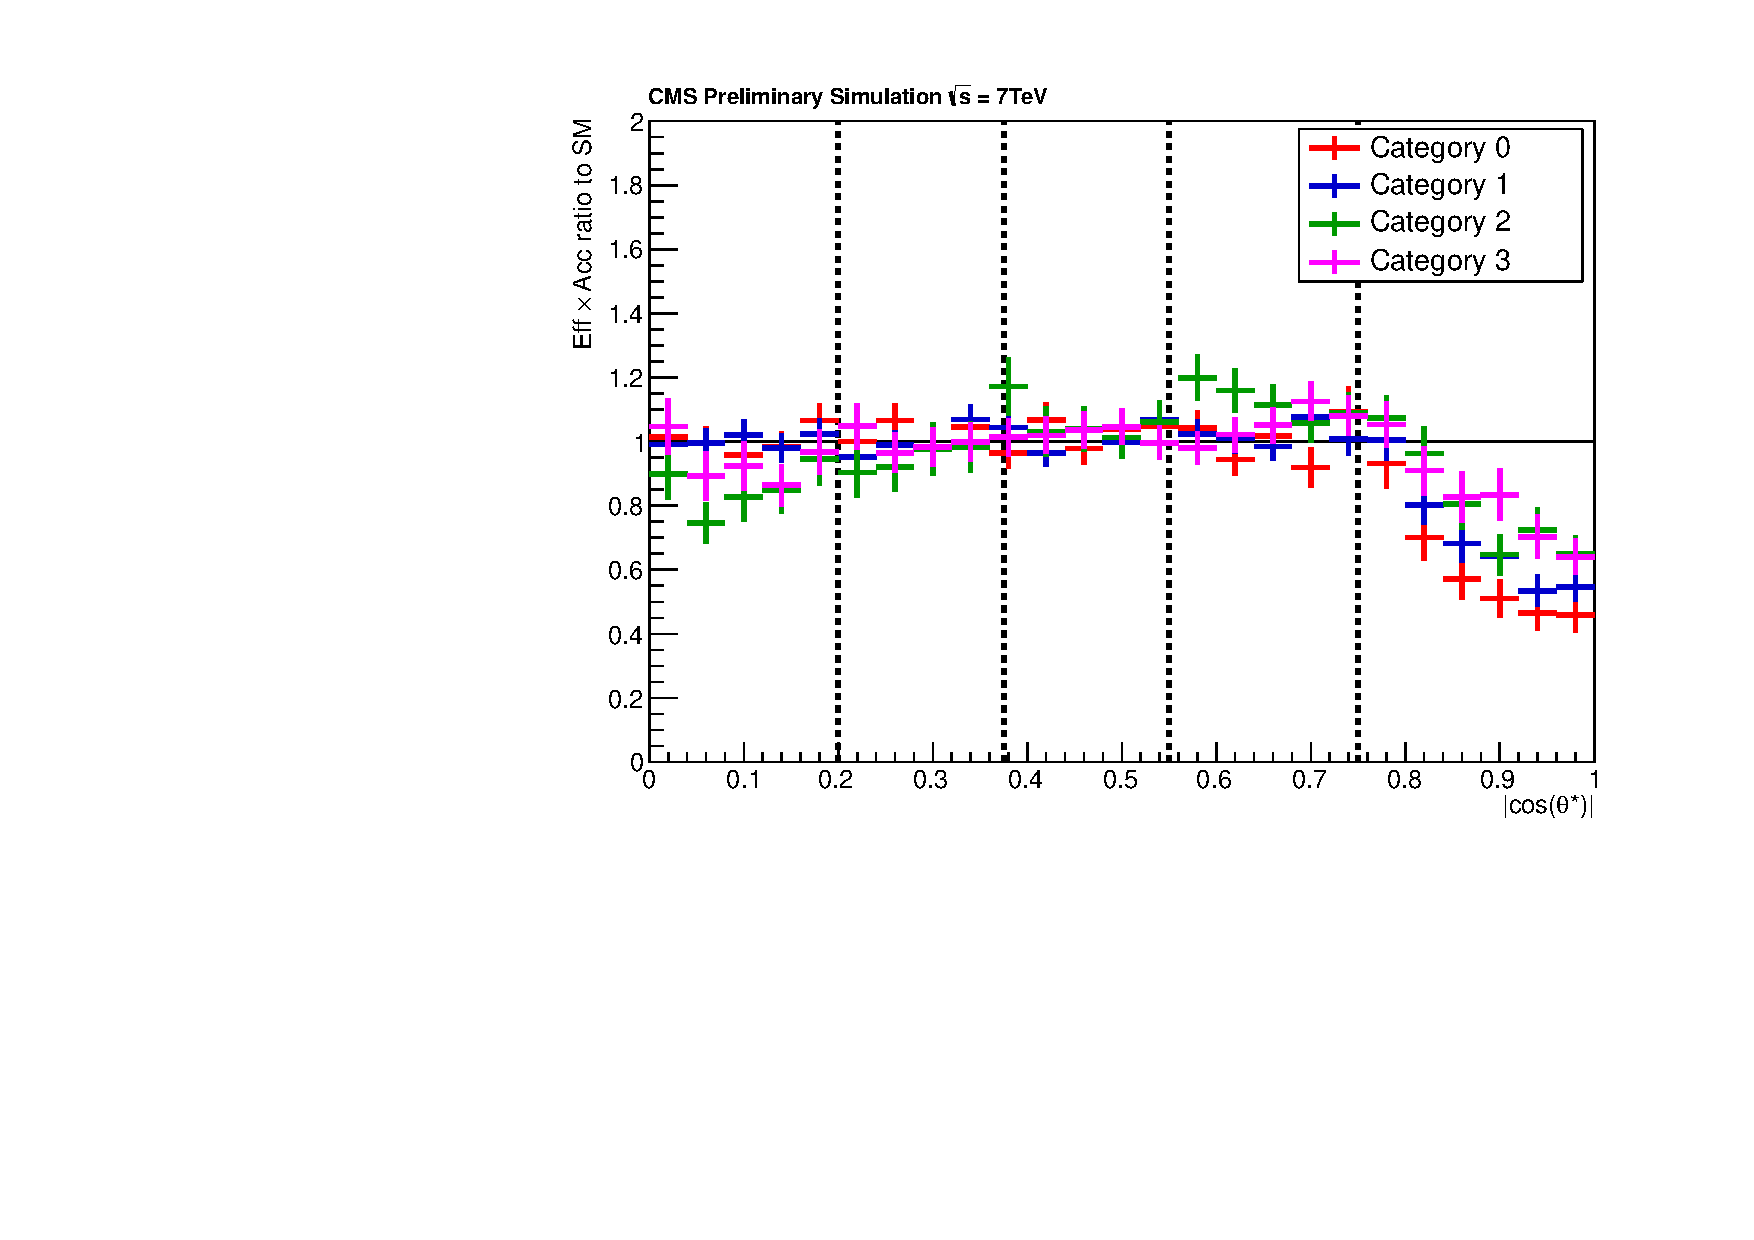
\includegraphics[width=0.49\linewidth]{ch6_spin_anal/plots/effacccats_7TeV.pdf}
	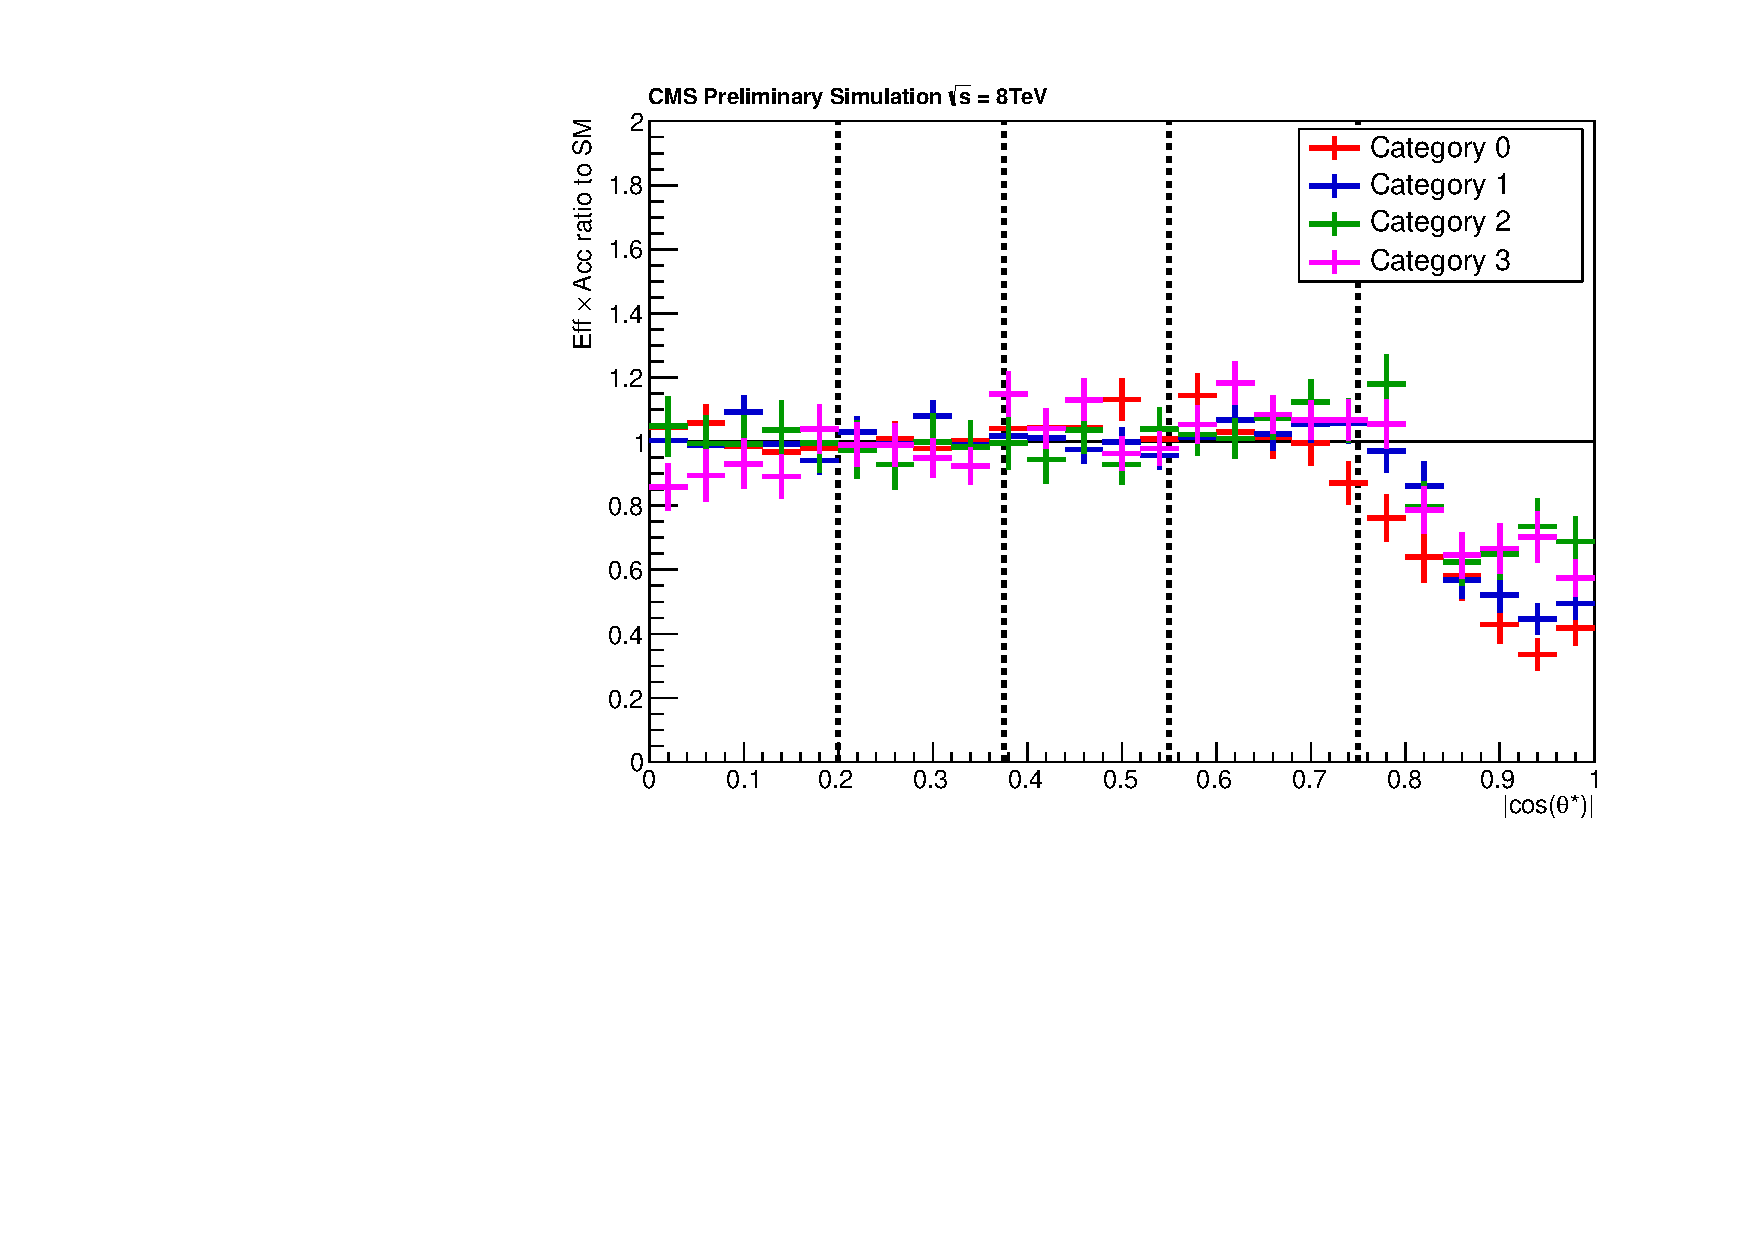
\includegraphics[width=0.49\linewidth]{ch6_spin_anal/plots/effacccats_8TeV.pdf}
  \caption{Acceptance $\times$ efficiency ratio between the \twomp (gluon-fusion production) and \zerop (all SM production modes) of the event selection as a function of \abscostheta split into the $|\eta|$ and $R_{9}$ categories defined in Table.~\ref{table:cats1}. The \abscostheta category boundaries are shown as the black dashed lines. The left hand plot is for the 7~\TeV \MC and the right hand plot for the 8~\TeV.}
	\label{fig:eff_acc}
	\end{center}
\end{figure}	


To benefit from the improved energy resolution of non-showering photons in 
the barrel, each event is categorised in $\eta$ and $R_{9}$ according to Table~\ref{table:cats1}.

\begin{table}
  \begin{center}
    \begin{tabular}{| l | l l l |}
      \hline
      Category 0 & $|\eta|_{\mbox{\tiny{max}}}<1.5$ & and & $R_{9\mbox{\tiny{min}}}>0.94$ \tabularnewline 
      Category 1 & $|\eta|_{\mbox{\tiny{max}}}<1.5$ & and & $R_{9\mbox{\tiny{min}}}\leq0.94$ \tabularnewline 
      Category 2 & $|\eta|_{\mbox{\tiny{max}}}>1.5$ & and & $R_{9\mbox{\tiny{min}}}>0.94$ \tabularnewline 
      Category 3 & $|\eta|_{\mbox{\tiny{max}}}>1.5$ & and & $R_{9\mbox{\tiny{min}}}\leq0.94$ \tabularnewline
      \hline
    \end{tabular}
    \caption{Definition of photon resolution categories}
    \label{table:cats1}
  \end{center}
\end{table}

%\begin{tabular}{l l l l l}
%  \textbullet & Category 0: & $|\eta|_{\mbox{\tiny{max}}}<1.444$ & and & $R_{9\mbox{\tiny{min}}}>0.94$ \\ 
%  \textbullet & Category 1: & $|\eta|_{\mbox{\tiny{max}}}<1.444$ & and & $R_{9\mbox{\tiny{min}}}\leq0.94$ \\ 
%  \textbullet & Category 2: & $|\eta|_{\mbox{\tiny{max}}}>1.444$ & and & $R_{9\mbox{\tiny{min}}}>0.94$ \\ 
%  \textbullet & Category 3: & $|\eta|_{\mbox{\tiny{max}}}>1.444$ & and & $R_{9\mbox{\tiny{min}}}\leq0.94$ \\
%\end{tabular}

Within each category events are binned in \abscostheta, to discrimate between the different spin hypotheses, according to Table.~\ref{table:cats2}.

\begin{table}
  \begin{center}
    \begin{tabular}{| l | r l |}
      \hline
      Spin Category 0 &             & \abscostheta $<0.2$ \tabularnewline 
      Spin Category 1 & $0.2\leq$   & \abscostheta$<0.375$ \tabularnewline 
      Spin Category 2 & $0.375\leq$ & \abscostheta$<0.55$ \tabularnewline 
      Spin Category 3 & $0.55\leq$  & \abscostheta$<0.75$ \tabularnewline 
      Spin Category 4 & $0.75\leq$  & \abscostheta$<1.0$ \tabularnewline 
      \hline
    \end{tabular}
    \caption{Definition of photon \abscostheta categories}
    \label{table:cats2}
  \end{center}
\end{table}


The \abscostheta boundaries are optimised to make particular use of the most disciminating 
bin (high \abscostheta) and to maintain uniform acceptance $\times$ efficiency in the 
other bins. In total the analysis is split into 20 event classes (4 $\eta$/\rnine\xspace 
categories $\times$ 5 \abscostheta categories) in each year which gives a total of 40 event classes.

\section{Signal and Background modelling}

The signal models are obtained from \MC simulation as described in Sec.~\ref{sec:mc} for the spin-0 \SM processes and the spin-2 processes. A parametric model identical to the one built for the nominal analysis is constructed as per the method described in Sec.~\ref{sec:signal_mfm}. The signal model is then parametrised as before in terms of $\mu$, \mH and two additional parameters, $x$ and \fqqbar, which dictate the amount of signal from spin-2 and the amount of spin-2 from $q\bar{q}$ production. The signal model parametrisation can be written as,

\begin{equation}
  \textbf{S}(m_{H},fqq,x;\hat{\theta}) = (1-x)\cdot\boldsymbol{S_{SM}}(m_{H};\hat{\theta})  + x\cdot\Bigl[f_{q\bar{q}}\cdot \boldsymbol{S_{q\bar{q}}}(m_{H};\hat{\theta}) + (1-f_{q\bar{q}})\boldsymbol{S_{gg}}(m_{H};\hat{\theta})\Bigr],  
  \label{eq:spin_sig}
\end{equation}

where $x$ is the amount of signal originating from spin-2, \fqqbar is the amount of spin-2 signal originating from $q\bar{q}$ production, \mH is the signal position and $\theta$ are the nuisance parameters.

The background model for the spin analysis comes in two forms. For the differntial measurement of the signal strength in bins of \abscostheta the envelope background method is used as per the description in Sec.~\ref{sec:envelope}. However, when calculating the statistical separation between various spin hypotheses a single parametrisation of the background is used in each category, namely a polynomial in the Bernstein basis~\cite{bernsteins1,bernsteins2} as per the description in eq.~\ref{eq:bernsteins}. The reason for this is that there is no asymptotic approximation for the test statistic distribution when the null hypothesis is not embedded in the alternative hypothesis. Consequently, in order to obtain the test statistic distributions (like the ones shown in Fig.~\ref{fig:cls}) one has to generate lots of pseudo-data and then refit this data to obtain the likelihood ratio and hence test statistic value. Given the complexity of the spin signal model and the combinatorics involved when using the envelope method with 40 analysis categories this becomes CPU impractical. It has been trialled using the GRID computing network but was found to take the order of hundreds of CPU years.
Given this complication and the fact that small losses in sensitivity to the background normalisation have a small impact on the spin hypothesis separation power a single parametrisation in each category was chosen for ease and simplicity. The choice is to use 4th order Bernstein polynomials in all categories apart from the highest \abscostheta star categories in which a 3rd order was chosen. The motivation behind this choice is that these order of polynomials show a similar level of bias as the envelope method when tested against ``truth" models for the spin categories analogous to the description in Sec.~\ref{sec:envelope}.

\section{Results}
\label{sec:spin_results}

The acceptance $\times$ efficiency of the two spin models in each category as well as the differential cross section as a function of \abscostheta, which depends only on the spin of the initial state, is obtained from the MC simulation. The only remaining assumption is on the total number of expected signal events for a given spin-parity state and production mode. This is well defined for the spin-0 SM case and is obtained from the $\sigma\times BR$ given by the LHC Higgs cross section working group in Ref.~\cite{LHCHiggsCrossSectionWorkingGroup3}. For the graviton-like \twomp this quantity is unknown. 
%Consequently, when generating pseduo-experiments for a particular model, the model is first fitted to the data to extract the relative shapes and normalisations of the signal and background. 
Consequently we scale the signal models for both spin hypotheses with a modifier, $\mu$, such that when $\mu=1$ and all \costhetastar information is ignored, the total number of expected signal events for the model in question is equivalent to the SM expectation. 
When generating pseduo-experiments for a particular model, the value of all the free parameters in the fit (including the signal nuisance parameters, the background shape parameters and the signal srength $\mu$) are set to their best fit values after fitting the model in question to the data.
In this way the expected separation is a fair representation of what we observe in data.

\subsection{SM compabibility check}
The signal yield, $\mu=\sigma/\sigma_{SM}$, is extracted independently in each of the \abscostheta bins, 
simultaneously fitting over the $\eta$ and \rnine bins such that the relative yields in each of the $\eta$ and \rnine 
bins is constrained to that predicted by the SM. The result is shown in Figure~\ref{fig:channelcomp} for the data (black points), the \zerop model expectation (red line), the \twomp model expectation using the $gg$ production mode only (blue line), the \twomp model expectation using the $q\bar{q}$ production mode only (green line) and the \twomp model expectation using a half-half mixture of $gg$ and $q\bar{q}$ production (magenta line), where for the expectations a single representative toy is used, obtained using asymptotic formulae from Ref.~\cite{asymptotic_form}, and the normalisation is extracted from a fit to data. The final point of the blue line can be understood
by referring back to Figure~\ref{fig:eff_acc}. The fact that the SM $ggH$ and $qqH$ production is of a similar strength at high values of \abscostheta causes the 
fitted strength (when fitting the \zerop model to the \twomp($gg$) expectation) to be smaller in the highest \abscostheta bin as compared to the second highest, contrary to what might be expected. 

\begin{figure}
  \begin{center}
    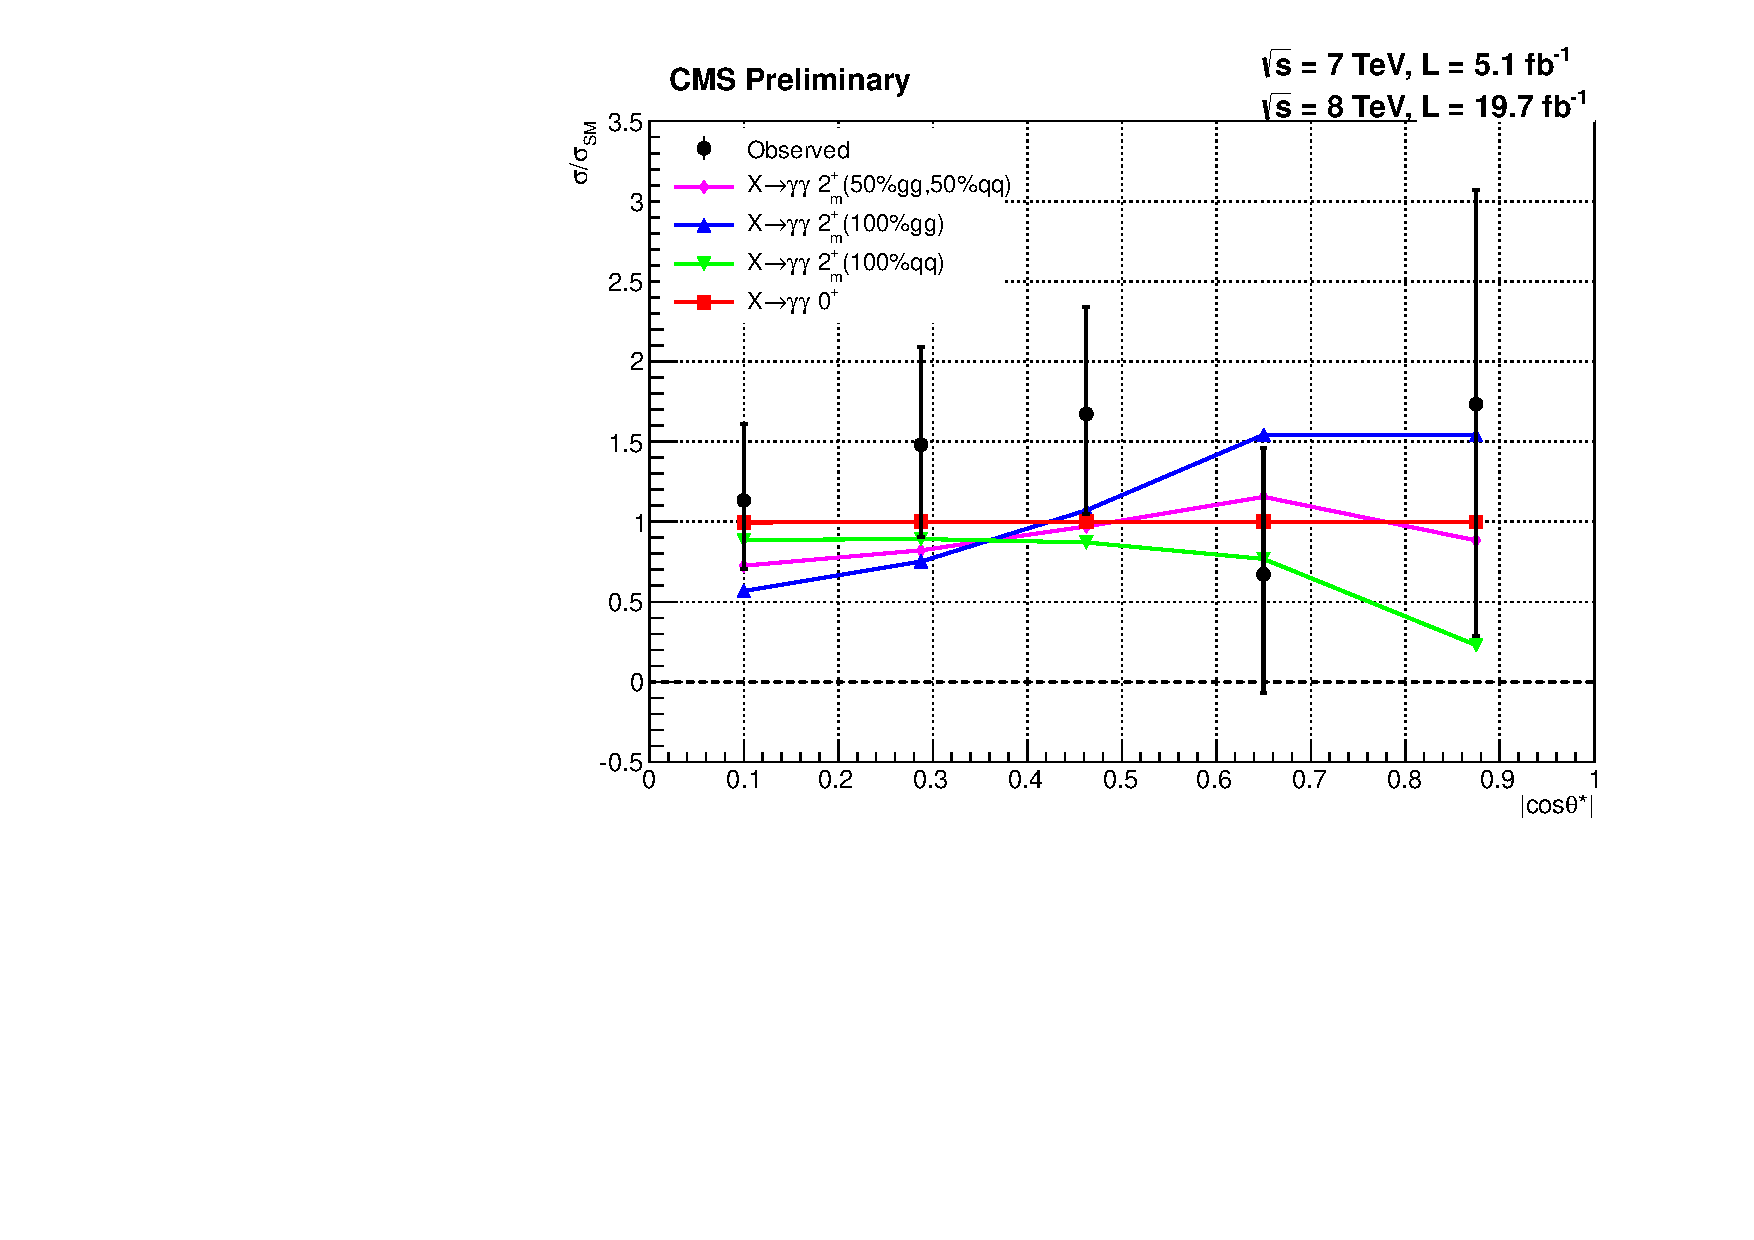
\includegraphics[width=0.8\linewidth]{ch6_spin_anal/plots/ch_comp_multipdfcomb_unblind.pdf}
    \caption{The SM extracted signal yield as a function of \abscostheta for the \zerop expectation (red line), \twomp expectation with gluon-fusion production only (blue line), the \twomp expectation with quark-antiquark annihilation production only (green line), the \twomp expectation with half $gg$, half $q\bar{q}$ production (magenta line) and the observation (black points).}
    \label{fig:channelcomp}
  \end{center}
\end{figure}

\subsection{Hypothesis tests of the SM Higgs, \zerop, vs. graviton-like, \twomp}
\label{sec:spin_separation}

The separation between the two models and the data is extracted using the test statistic defined as twice the negative ratio 
of the likelihoods for the \zerop signal plus background hypothesis and the \twomp signal plus background hypothesis when 
performing a simultaneous fit of all twenty event classes together, $q=-2\,{\ln({\cal L}_{2^{+}_\mathrm{m} + \mathrm{bkg.}}/{\cal
L}_{0^+ + \mathrm{bkg.}})}$.

The distribution of this test statistic is shown in 
Fig.~\ref{fig:separation} for pseudoexperiments generated with an overall signal yield and signal position which is extracted from a fit to the data for
the \zerop hypothesis (orange) 
and the \twomp hypothesis (blue) for gluon-fusion production only (left) and quark-antiquark annihilation production only (right). The observed value is shown as the red arrow. The 1-$CL_{s}$ observed exclusion for a gluon-fusion only produced spin-2 boson is 93.7\% whilst for quark-antiquark produced boson is 85.0\%. 

\begin{figure}
  \begin{center}
    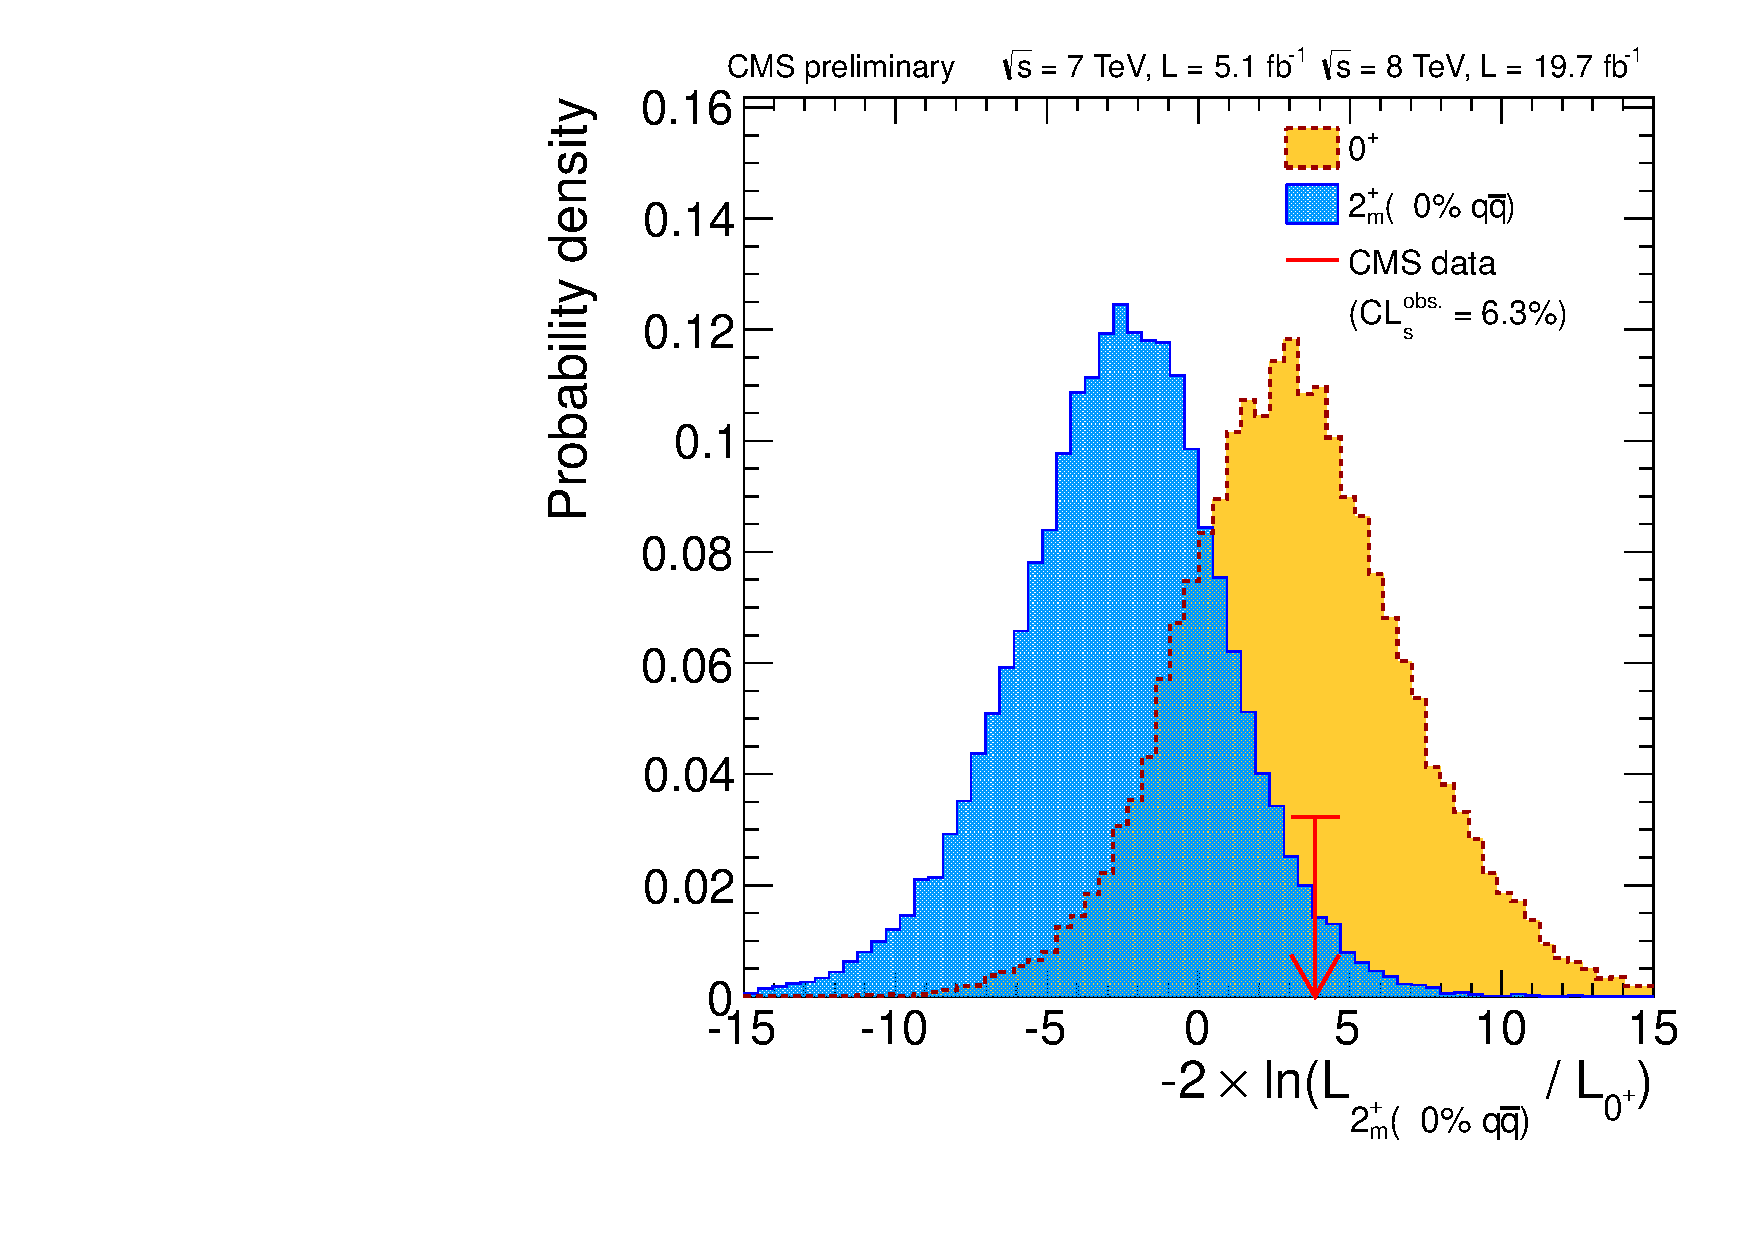
\includegraphics[width=0.49\linewidth]{{ch6_spin_anal/plots/2pm0.00_unblind}.pdf}
    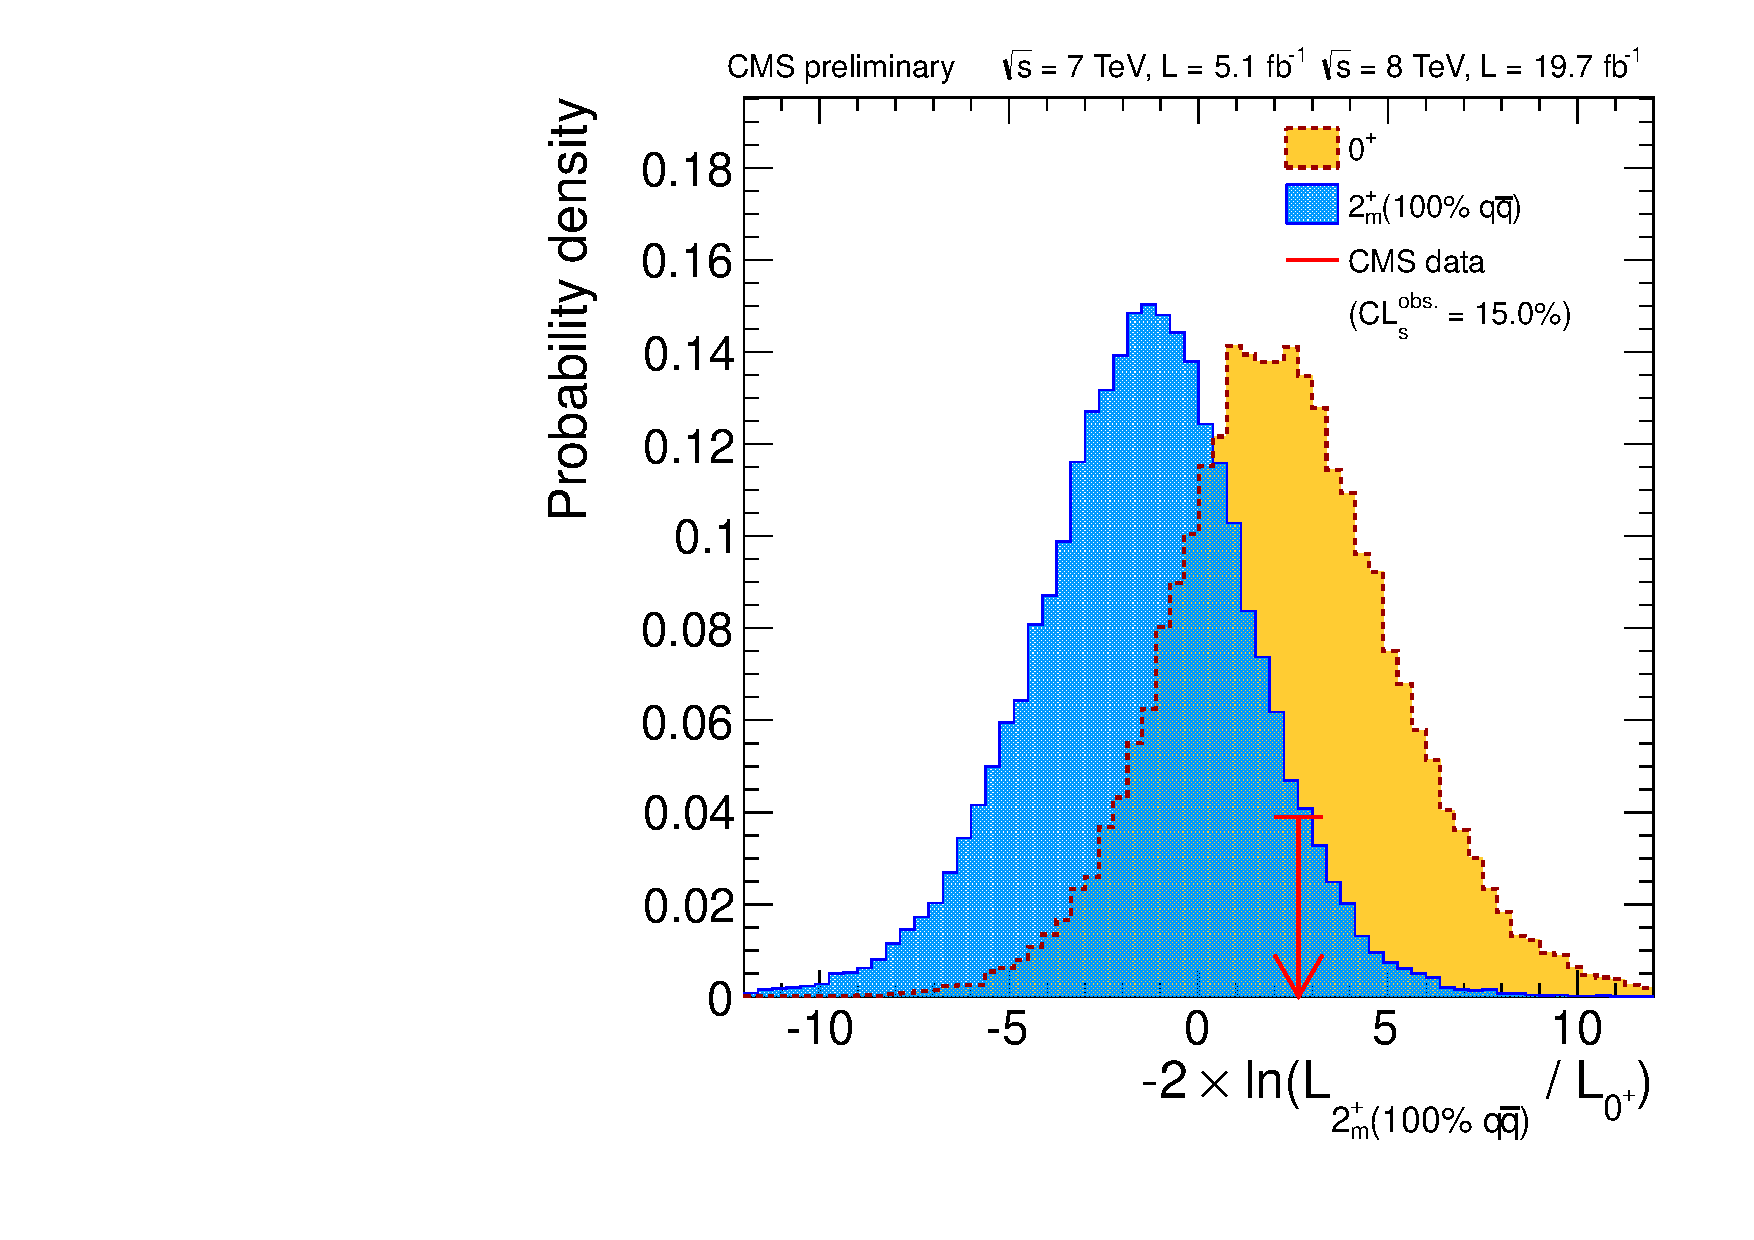
\includegraphics[width=0.49\linewidth]{{ch6_spin_anal/plots/2pm1.00_unblind}.pdf}
    \caption{The distribution of the test statistic for pseudo experiments generated under the SM, \zerop, hypothesis (orange) and the \emph{graviton-like}, \twomp, hypothesis (blue) with gluon fusion produciton only (left) and quark-antiquark production only (right). The observed value in the data is shown as the red arrow.}
    \label{fig:separation}
  \end{center}
\end{figure}

The previous two tests are both performed assuming that the \twomp state is produced entirely by either gluon-fusion or quark-antiquark annihilation. A further three points, with mixtures of $gg$ and $q\bar{q}$ spin-2 production, have been tested such that the overall yield of the \twomp signal is fixed to the best fit value of the model in question to data and the fraction of \qqbar production is increased by a factor, \fqqbar. Figure~\ref{fig:qqbar} shows the distribution of the test statistic as a function of the fraction of \twomp production from $q\bar{q}$ annihilation. Figure~\ref{fig:separation} is, in effect, a projection of Fig.~\ref{fig:qqbar} at the points \fqqbar=0\% and \fqqbar=100\%. It can be seen that the data is very much in line with the \SM expectation. Whilst \textit{a prior} it may look as though the data points in Fig.~\ref{fig:qqbar} lie to close to the \SM mean (red line) all of these points are highly correlated. If the data look flat in \abscostheta then they will look flat for all values of \fqqbar. In this sense the green and yellow bands in Fig.~\ref{fig:qqbar} can be misleading.

\begin{figure}
  \begin{center}
    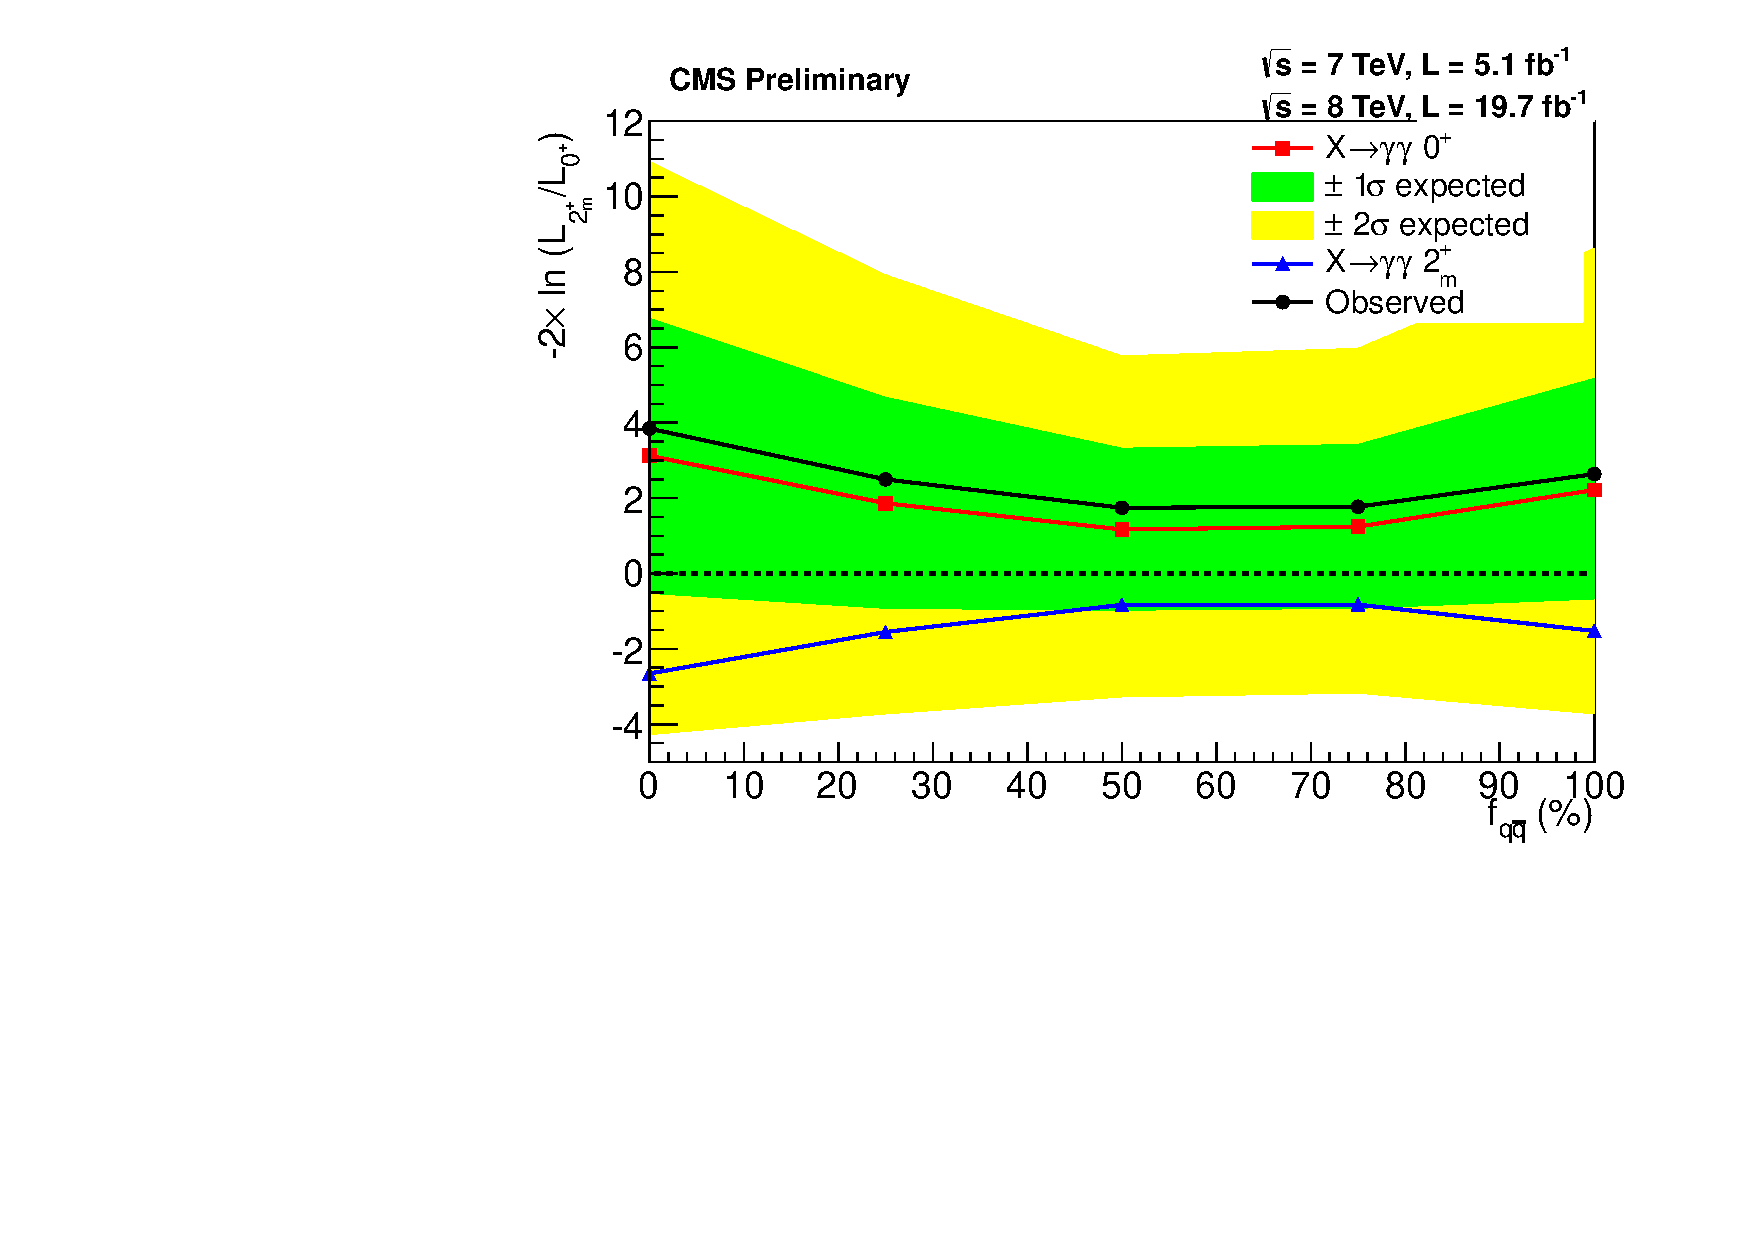
\includegraphics[width=0.8\linewidth]{ch6_spin_anal/plots/fqqbar_unblind.pdf}
    \caption{The distribution of the test statistic for pseudo experiments thrown under the SM, \zerop, hypothesis (red) and the \emph{graviton-like}, \twomp, hypothesis (blue) as a function of the fraction of \qqbar production relative to $gg$ production. The observed distribution in the data is shown by the black points.}
    \label{fig:qqbar}
  \end{center}
\end{figure}




  \input{ch7_concs/ch7_concs}
\end{mainmatter}

%% Produce the appendices
\begin{appendices}
  %%% The "\appendix" call has already been made in the declaration
%% of the "appendices" environment (see thesis.tex).
\chapter{Pointless extras}
\label{app:Pointless}

\chapterquote[french]%
{Le savant n'\'etudie pas la nature parce que cela est utile; \\
\indent il l'\'etudie parce qu'il y prend plaisir, \\ 
\indent et il y prend plaisir parce qu'elle est belle.}%
{Henri Poincar\'e, 1854--1912}

Appendixes (or should that be ``appendices''?) make you look really clever, 'cos
it's like you had more clever stuff to say than could be fitted into the main
bit of your thesis. Yeah. So everyone should have at least three of them\dots

\section{Like, duh}
\label{sec:Duh}
Padding? What do you mean?

\section{$y = \alpha x^2$}
\label{sec:EqnTitle}
See, maths in titles automatically goes bold where it should (and check the 
table of contents: it \emph{isn't} bold there!) Check the source: nothing
needs to be specified to make this work. Thanks to Donald Arsenau for the
teeny hack that makes this work.

%% Big appendixes should be split off into separate files, just like chapters
%\input{app-myreallybigappendix}

\end{appendices}

%% Produce the un-numbered back matter (e.g. colophon,
%% bibliography, tables of figures etc., index...)
\begin{backmatter}
  %\begin{colophon}
  %This thesis was made in \LaTeXe{} using the ``hepthesis'' class~\cite{hepthesis}.
%\end{colophon}

%% You're recommended to use the eprint-aware biblio styles which
%% can be obtained from e.g. www.arxiv.org. The file mythesis.bib
%% is derived from the source using the SPIRES Bibtex service.
\bibliographystyle{h-physrev}
\bibliography{mythesis}

%% I prefer to put these tables here rather than making the
%% front matter seemingly interminable. No-one cares, anyway!
\listoffigures
\listoftables

%% If you have time and interest to generate a (decent) index,
%% then you've clearly spent more time on the write-up than the 
%% research ;-)
%\printindex

% declare acronyms
\newpage
\thispagestyle{empty}
\phantomsection
\addcontentsline{toc}{chapter}{List of Acronyms}
\vspace*{1.95cm} \hspace*{-0.155cm} %,88
\textbf{{\huge List of Acronyms}\\}
\vspace*{0.5cm}
\begin{acronym}[AAAAAA]
\acro {BDT} [BDT] {Boosted Decision Tree}
\acro {BDTs} [BDTs] {Boosted Decision Trees}
\acro {CERN} [CERN] {European Organization for Nuclear Research}
\acro {CMS} [CMS] {Compact Muon Solenoid}
\acro {ECAL} [ECAL] {Electromagnetic calorimeter}
\acro {HCAL} [HCAL] {Hadronic calorimeter}
\acro {LHC} [LHC] {Large Hadron Collider}
\acro {MVA} [MVA] {Multivariate analysis}
\acro {MVAs} [MVAs] {Multivariate analyses}
\acro {CiC} [CiC] {Cuts in Categories}
\acro {MFM} [MFM] {Mass Factorized MVA}
\acro {MBM} [MBM] {Mass Blind MVA}
\acro {SMVA} [SMVA] {Sideband MVA}
\acro {SM} [SM] {Standard Model}
\acro {PbWO} [PbWO$_{4}$] {lead tungstate}
\acro {APD} [APD] {avalance photodiode}
\acro {APDs} [APDs] {avalance photodiodes}
\acro {VPTs} [VPTs] {vacuum phototriodes}
\acro {GED} [GED] {global event description}
\end{acronym}





\end{backmatter}

%% Close
\end{document}
